% ============================================================
%  Hyperion SLT+Adam Style Transfer — TPAMI submission
%  Compile: pdflatex main -> bibtex main -> pdflatex -> pdflatex
% ============================================================
\documentclass[10pt,journal,compsoc]{IEEEtran}

\usepackage{amsmath,amssymb,amsfonts,mathtools}
\usepackage{graphicx}
\usepackage{booktabs}
\usepackage{multirow}
\usepackage{algorithm}
\usepackage{algpseudocode}
\usepackage[table]{xcolor}
\definecolor{tabshade}{HTML}{3E7FB8} % value-mapped cell shading in result tables
\usepackage{subcaption}
\usepackage{microtype}
\usepackage{enumitem}
\usepackage[
  colorlinks=true,
  linkcolor=blue!60!black,
  citecolor=green!50!black,
  urlcolor=blue!70!black,
  filecolor=blue!70!black,
]{hyperref}
\usepackage[capitalise,noabbrev]{cleveref}
% Override cleveref names to use IEEE-style abbreviations
\crefname{figure}{Fig.}{Figs.}
\Crefname{figure}{Fig.}{Figs.}
\crefname{table}{Table}{Tables}
\Crefname{table}{Table}{Tables}
\crefname{section}{Sec.}{Secs.}
\Crefname{section}{Sec.}{Secs.}
\crefname{equation}{Eq.}{Eqs.}
\Crefname{equation}{Eq.}{Eqs.}
\usepackage{dblfloatfix}   % fixes figure* placement in two-column IEEEtran

% Relax float placement constraints (IEEEtran defaults are too strict)
\renewcommand{\topfraction}{0.9}
\renewcommand{\bottomfraction}{0.5}
\renewcommand{\textfraction}{0.07}
\renewcommand{\floatpagefraction}{0.7}
\renewcommand{\dbltopfraction}{0.9}
\renewcommand{\dblfloatpagefraction}{0.7}
\usepackage{placeins}  % \FloatBarrier keeps each section's floats inside it
\usepackage{float}     % [H] pins small charts inline (no blank float pages)
\usepackage{balance}   % 十修排版: balance the last references page's columns

% ---- theorem environments ----
\usepackage{amsthm}
\newtheorem{theorem}{Theorem}[section]
\newtheorem{proposition}[theorem]{Proposition}
\newtheorem{assumption}{Assumption}[section]
\newtheorem{remark}{Remark}[section]
% ---- paper-wide macros ----
\newcommand{\TODO}[1]{{\color{red}\textbf{[TODO: #1]}}}
\newcommand{\REV}[1]{#1}% submission build: revision trace neutralized
\newcommand{\etal}{\textit{et~al.}}
\newcommand{\LRS}{\textsc{lrs}}
\newcommand{\Lsty}{\mathcal{L}_{\mathrm{sty}}}
\newcommand{\Lcnt}{\mathcal{L}_{\mathrm{cnt}}}
% 九修: unnumber \paragraph{} run-ins (advisor: drop 3.9.0.1-style numbers)
\setcounter{secnumdepth}{3}
% 十一修 评阅#5: IEEEtran(compsoc) 的 \paragraph 缩进是 2\parindent（老师圈的
% 大缩进），改为零缩进；其余间距/字体保持类默认。标题内的句号/问号已全文清除
% （类自动补冒号，原先渲染成 "Notation.:"）。
\makeatletter
\def\paragraph{\@startsection{paragraph}{4}{\z@}%
  {-0ex plus -0.1ex minus -0.1ex}{0ex}{\normalfont\normalsize}}
\makeatother
% ---------------------------

% 2026-07-03 九修: title + method name "Hyperion" (= the SLT + Adam-in-loop
% + LRS pipeline; the old name was "Hy-brid", renamed globally, 106 sites,
% mechanical rename NOT \REV-wrapped) per the advisor's direction.
\title{Bridging the Training Gap with Hyperion: A Training-Free Style
Transfer Method on Diffusion Transformers}

\author{Yi~Li, Chengyan~Li, Zhirui~Fang, Junchuan~Zhang, Xuan~Wang, Huaibo~Huang, Yan~Luo, and~Yanqing~Guo%
\IEEEcompsocitemizethanks{
\IEEEcompsocthanksitem Y. Li, C. Li, Z. Fang, J. Zhang, Y. Luo, and Y. Guo are with Dalian University of Technology, Dalian, China.\protect\\
E-mail: liyi@dlut.edu.cn, gggmdgzsx@mail.dlut.edu.cn, fangzr@mail.dlut.edu.cn, junchuanz@mail.dlut.edu.cn, 20211071090@mail.dlut.edu.cn, guoyq@dlut.edu.cn
\IEEEcompsocthanksitem X. Wang is with Beihang University, Beijing, China. E-mail: zb2506519@buaa.edu.cn
\IEEEcompsocthanksitem H. Huang is with the Institute of Automation, Chinese Academy of Sciences, Beijing, China. E-mail: huaibo.huang@cripac.ia.ac.cn
}%
}

\begin{document}

\maketitle

% 十二修 (2026-07-09): abstract re-polished per advisor (师兄) — adds the
% "optimization level / distribution level" framing and tightens the prose.
% Numbers unchanged and CANONICAL-consistent (full 234-pair 0.640/0.296;
% +5.2% vs Adam-8; +16.6% equal-budget; 19/21; mean 0.657 vs 0.506).
% Supersedes the 九修 advisor revision.
\begin{abstract}
Training-free style transfer on Multimodal Diffusion Transformers (MM-DiT)
remains challenging due to the persistent gap between trained adapters and
injection-based training-free methods.
Existing training-free methods typically perform forward feature injection, and
thus struggle to reproduce the rich painterly textures achieved by trained
adapters, often leading to only faint hue shifts.
In this paper, we trace this limitation to the absence of
backpropagation-induced spatial coupling and propose \textbf{Hyperion}, a fully
training-free style-transfer pipeline for MM-DiT.
At the optimization level, the pipeline introduces \textbf{Adam-in-loop}, which
iteratively optimizes the diffusion latent at each denoising step with a frozen
MM-DiT.
This process recovers the gradient-driven coupling effect produced through the
self-attention \emph{value path}, where neighboring tokens receive highly
similar updates and form coherent brushstroke textures.
At the distribution level, the pipeline introduces \textbf{Sinkhorn Latent
Transport (SLT)}, a single closed-form optimal-transport step that pre-aligns
latent color distributions before Adam optimization, improving the operational
efficiency of Adam-in-loop.
To further enhance stylization quality, we develop a frequency-domain Sinkhorn
loss to sharpen painterly textures and a layout-residual-suppression step to
reduce layout interference.
The pipeline can also be extended to image-to-image stylization.
Extensive experiments on a 39-style $\times$ 6-prompt benchmark (234 pairs)
demonstrate that Hyperion achieves CSD~$= 0.640$ and CLIP-T~$= 0.296$,
improving CSD by \textbf{+5.2\%} over Adam-8 at $2.5\times$ lower forward-pass
cost and by \textbf{+16.6\%} over Adam-only under an equal compute budget.
Notably, Hyperion outperforms four pre-trained style adapters on \textbf{19 of
21} diverse style families, achieving a mean CSD of $0.657$ versus $0.506$ for
the strongest baseline.
\end{abstract}

\begin{IEEEkeywords}
style transfer, diffusion transformers, optimal transport, latent optimization,
training-free generation
\end{IEEEkeywords}

\section{Introduction}
\label{sec:intro}

\begin{figure*}[t]
  \centering
  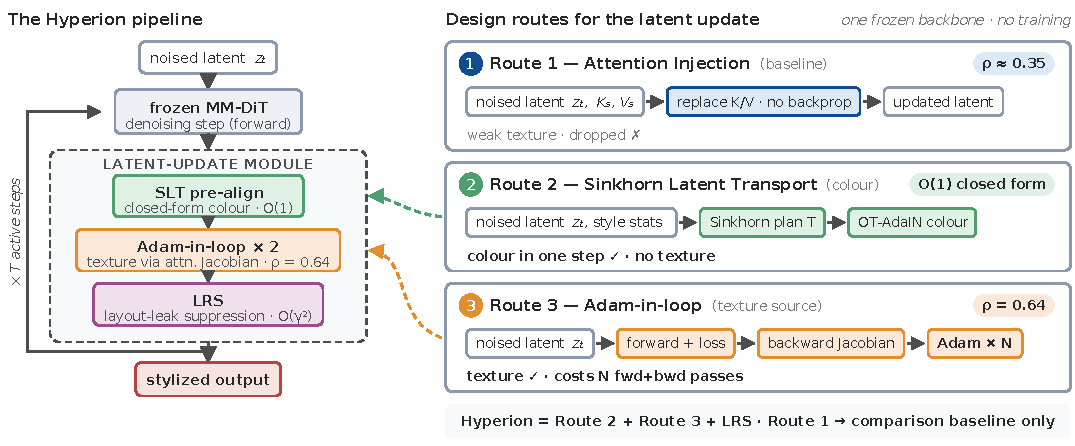
\includegraphics[width=\linewidth]{fig/figure/fig_framework_v3.pdf}
  \caption{%
    Design space of the method. \emph{Left} (dashed box = latent-update
    module): the final integrated
    \textbf{Hyperion pipeline}---at each active denoising step the frozen MM-DiT
    runs a style forward pass, SLT pre-aligns color in one closed-form step,
    two Adam steps inject cross-token texture through the self-attention
    Jacobian ($\rho{=}0.64$), and LRS suppresses layout leakage.
    \emph{Right}: the three latent-update design routes, each shown as a detailed
    module framework---\textbf{Route~1} Attention Injection (the training-free
    baseline that replaces content $K/V$ with style $K/V$ in one block, no
    backprop; $\rho{\approx}0.35$, weak texture); \textbf{Route~2}
    Sinkhorn Latent Transport (closed-form color alignment, $O(1)$, no
    texture); and \textbf{Route~3} Adam-in-loop (backprop through the frozen
    backbone, the source of spatial coherence, $\rho{=}0.64$). The Hyperion
    integrates Route~2 and Route~3 (with LRS layout suppression), discarding
    the injection baseline.%
  }
  \label{fig:architecture}
\end{figure*}

% ── Para 1: 鸿沟 ─────────────────────────────────────────────────────────────
Style transfer on modern image generation models falls into two
regimes that have so far remained largely separate.
\emph{Trained} methods (fine-tuned adapters, ControlNet-style
encoders~\cite{ipadapter2023,zhang2023controlnet,megastyle2026,xing2024csgo}) % 十修: remix2025 placeholder citation removed (unverifiable)
inject a style reference into the model's weights or cross-attention banks via
gradient descent, achieving high semantic fidelity and rich painterly texture.
\emph{Training-free} methods (attention $K/V$ injection, token
substitution, latent interpolation~%
\cite{hertz2024style,chung2024styleid,zhang2023inst,vshuffle2025,dualrf2025,xu2025stylessp,lin2025freecontrol})
require no optimization and generalize immediately to any reference image, but
their outputs exhibit only faint hue shifts with no discernible texture
structure, and their style fidelity—measured by the Contrastive Style
Descriptor (CSD)~\cite{somepalli2024measuring}—falls far below that of their
trained counterparts.
We argue that this gap originates from the underlying mechanism
rather than from model scale or training data (Sec.~\ref{sec:method:gap}).

% ── Para 2: 溯因 ─────────────────────────────────────────────────────────────
We investigate \emph{why} trained style methods produce coherent
texture while training-free ones do not, and attribute the difference to the
backpropagation graph.
It is well established that self-attention keys and values in diffusion
transformers encode both semantic content and fine-grained visual
texture~\cite{hertz2022prompt,chung2024styleid,seg4diff2025,gan2025ditf};
manipulating $K/V$ during denoising has therefore become the standard
mechanism for lightweight style injection~\cite{hertz2024style,xu2025stylessp}.
During fine-tuning, however, gradients flow back through the full diffusion
transformer and through its multi-head self-attention
Jacobian~\cite{vaswani2017attention}.
Neighboring tokens carry nearly identical keys—a structural consequence of
spatial continuity in the RoPE-encoded latent
grid~\cite{su2024rope,esser2024scaling}—so the rest of the image attends to
them with nearly equal weights; and because each token's output is a weighted
blend of value vectors, backpropagation through this \emph{value path}
therefore delivers nearly identical gradient signals to spatially adjacent
tokens, causing their latent updates to point in the same direction.
This spatial coherence is precisely what constitutes brushstroke texture:
it mirrors the long-range spatial correlations that Gatys
\etal~\cite{gatys2016image} identify as the defining statistical signature of
painterly style, now produced not by Gram-matrix optimization but as a natural
by-product of the attention Jacobian during backpropagation.
We make this claim precise in two ways: formally, by proving that
spatially smooth content keys force adjacent tokens to receive near-identical
gradient directions (Sec.~\ref{sec:method:gap},
Appendix~\ref{app:jacobian}); and empirically, by introducing the
\emph{spatial neighbor cosine}, a measure of how strongly adjacent per-token
updates align, under which backward-pass gradients prove far more spatially
coherent than any feedforward training-free update.
Training-free methods, because they perform no backward pass, lack this
cross-token coupling mechanism entirely.

% ── Para 3: 弥合 ─────────────────────────────────────────────────────────────
This observation suggests a direct remedy: \emph{introducing
backpropagation into the training-free setting}.
Starting from a standard inversion-interpolation baseline that blends content
and style attention features without any
optimization~\cite{hertz2024style,chung2024styleid,xu2025stylessp,avrahami2025stableflow},
we add an iterative Adam update~\cite{kingma2015adam} loop at each denoising
timestep.
At each step, a style forward pass extracts reference $K/V$ tensors; the
content latent is then updated by Adam on a style-alignment loss computed
from the content forward pass, with gradients flowing through the
self-attention Jacobian~\cite{vaswani2017attention}.
We call this \textbf{Adam-in-loop} style optimization.
To our knowledge, this is the first training-free pipeline on MM-DiT
whose outputs exhibit brushstroke texture, raising style fidelity from the
injection regime to a level comparable with trained adapters.

% ── Para 4: 速度瓶颈 ──────────────────────────────────────────────────────────
More iterations, however, mean slower generation: each Adam step costs a full
forward and backward pass through the model, and accumulated style pressure
gradually erodes faithfulness to the content
prompt~\cite{radford2021learning}.
Profiling the optimization reveals that the early iterations are
largely devoted to \emph{color distribution alignment}: the gradient is
dominated by a global low-frequency component that corrects bulk color
statistics, leaving only a small fraction of each step for the intended
texture signal.
Recent work confirms that high- and low-frequency components of diffusion
latents behave fundamentally differently during
generation~\cite{huang2025fresca,yuan2025consisid}, corroborating that a
single gradient step cannot serve both goals efficiently---a frequency
separation we later exploit directly through a frequency-domain Sinkhorn loss
(Sec.~\ref{sec:method:freq}).

% ── Para 5: OT 逼近 ──────────────────────────────────────────────────────────
This analysis reveals a mismatch between tool and task: gradient
descent is well suited to optimizing a differentiable objective through a
neural Jacobian, but poorly suited to global distribution alignment.
Color mismatch between the content and style latents is not a local,
high-curvature objective—it is a bulk statistical discrepancy between two
token populations~\cite{huang2017arbitrary}.
Optimal transport solves exactly this problem in closed form: it computes the
globally cost-minimizing assignment of content tokens to style tokens that
equates the two marginal
distributions~\cite{villani2009optimal,peyre2019computational,haviv2025wasserstein}.
Crucially, optimal transport does not pass through the attention Jacobian at
all—it operates directly in latent token space, bypassing the mechanism that
generates spatial coherence.
This property is precisely what is needed: optimal transport
resolves, in a single step, the sub-task that consumes most of Adam's
gradient budget, while leaving the Jacobian untouched for texture formation.
We implement this as \textbf{Sinkhorn Latent Transport (SLT)}, a soft
transport step driven by a doubly-stochastic Sinkhorn
plan~\cite{cuturi2013sinkhorn} whose marginal constraints guarantee that every
style token contributes to the result, preventing the mode collapse that
row-only softmax normalization permits~\cite{peyre2019computational}.
SLT matches color distributions at negligible cost; yet, used alone, its
outputs remain visually flat.
The reason is structural: the transport update at each token is independent of
every other token's update, so no mechanism couples adjacent positions, and
the spatially coherent structures that constitute brushstroke texture cannot
emerge (Sec.~\ref{sec:method:slt}).

% ── Para 6: Hyperion ───────────────────────────────────────────────────────────
The two mechanisms are complementary: SLT resolves what Adam
expends iterations on
(global color distribution via optimal
transport~\cite{villani2009optimal,haviv2025wasserstein}), while Adam produces
what SLT structurally cannot (cross-token gradient coupling via the
self-attention Jacobian~\cite{vaswani2017attention}).
Our \textbf{Hyperion} pipeline (Fig.~\ref{fig:architecture}) chains them within
each denoising step: SLT pre-aligns the color distribution, after which the
remaining Adam iterations are directed almost entirely toward texture.
We formalize this as a pre-alignment efficiency result
(Sec.~\ref{sec:method:hybrid}, Appendix~\ref{app:hybrid}) and confirm it
empirically: a Hyperion schedule with only two Adam iterations matches the
style fidelity of a far longer Adam-only schedule at a fraction of the
compute, and clearly outperforms Adam-only optimization at an equal compute
budget.

% ── Para 7: Contributions ─────────────────────────────────────────────────────
% 十一修 评阅#4: contribution 改 itemize、块内文献引用全部移除（各项均已在
% related work / method / experiments 相应位置引用）；随后的 Sec.2–7 路线图段
% 按老师意见删除。vaswani2017attention 在本节 Para 6 仍有引用，不失引。
\noindent\textbf{Contributions:}
\begin{itemize}[leftmargin=1.4em, itemsep=1pt, topsep=2pt]
  \item We identify the disparity between training-free and trained style
  transfer as a \emph{backpropagation gap}: trained methods derive spatial
  coherence from the self-attention Jacobian, whereas training-free injection
  methods lack this coupling entirely. We support this diagnosis with a formal
  coherence analysis and a reusable diagnostic, the \emph{spatial neighbor
  cosine} $\rho$, which we further extend to an output-image
  texture-coherence score (Sec.~\ref{sec:exp:texcoh}).
  \item We present \textbf{Hyperion}, a fully training-free style-transfer
  pipeline that bridges this gap by combining \textbf{Adam-in-loop} and
  \textbf{Sinkhorn Latent Transport (SLT)}. Adam-in-loop performs iterative
  backpropagation through a frozen MM-DiT at each denoising step, while SLT
  provides a closed-form optimal-transport color pre-alignment whose
  complementarity with Adam-in-loop is formally characterized.
  Frequency-domain Sinkhorn boosting and layout-residual suppression further
  enhance texture formation and suppress layout leakage.
  \item We validate Hyperion extensively on a 234-pair benchmark, where it
  raises CSD from $<0.15$ (injection) to $0.640$, exceeds an 8-iteration
  Adam-only schedule at $2.5\times$ lower forward-pass cost, outperforms four
  trained adapters on 19 of 21 style families, and extends effectively to
  image-to-image stylization. Controlled ablations further attribute the gains
  to the individual components.
\end{itemize}

\section{Related Work}
\label{sec:related}

% 十修: related work 由 7 个 subsection 合并精简为 4 个（作者指示）。原
% (1) Classical NST、(2) Training-free diffusion、(3) Content-style
% disentanglement、(4) Trained adapters、(5) Latent optimization、(6) Optimal
% transport、(7) DiT architecture 重组为：§2.1=1+2+7、§2.2=4+3、§2.3=5、
% §2.4=6。全部引用保留（仅删重复过渡句与各节冗余的局限性复述）；结构性
% 重组不整体 \REV，新写的衔接句以 \REV 标记。ReMix 占位引用此前已删。
Style transfer methods divide into two regimes---training-free \emph{injection}
and \emph{trained} adapters---separated by a persistent quality gap: injection
transfers color but little texture, while trained adapters achieve rich texture
at the cost of per-style optimization.
We trace this gap to a single missing ingredient, gradient feedback through the
self-attention value path (Sec.~\ref{sec:method:gap}), and close it with a
training-free pipeline combining Adam-in-loop optimization, Sinkhorn latent
transport, and layout residual suppression.
We organize the survey around this thesis, noting where each prior family sits
relative to it.

% ----------------------------------------------------------------
\subsection{Training-Free Style Transfer: from Gram Matrices to Attention
Injection}
% ----------------------------------------------------------------

Classical neural style transfer established the statistical view of
style that we build on.
Gatys \etal~\cite{gatys2016image} showed that Gram matrices of
VGG~\cite{simonyan2015vgg} features capture perceptual texture statistics;
feed-forward networks~\cite{johnson2016perceptual} amortized the per-style
cost, and AdaIN~\cite{huang2017arbitrary} reduced arbitrary style transfer to
channel-wise moment matching, later extended to whitening--coloring
transforms~\cite{li2017universal} and higher-order moments~\cite{hsi2025}.
These CNN-based methods operate on fixed VGG hierarchies and cannot
express the cross-token gradient coupling that we identify as the source of
brushstroke texture in modern diffusion
transformers~\cite{peebles2023scalable,dosovitskiy2021vit}---in particular
MM-DiT~\cite{esser2024scaling}, which processes image and text in jointly
attending streams under RoPE positional encoding~\cite{su2024rope} and whose
attention features encode high-fidelity spatial
semantics~\cite{seg4diff2025,gan2025ditf}.

Because self-attention keys and values in diffusion
models~\cite{ho2020denoising} encode both semantic content and
fine-grained texture~\cite{hertz2022prompt}, manipulating $K/V$ during
denoising is the standard training-free stylization pathway.
InST~\cite{zhang2023inst} encodes the style image in prompt space via textual
inversion; Prompt-to-Prompt~\cite{hertz2022prompt} established attention maps
as the central control knob for semantic manipulation.
StyleID~\cite{chung2024styleid} retains content queries while substituting
style $K/V$ with attention temperature scaling;
StyleAligned~\cite{hertz2024style} shares $K/V$ across a batch;
AttenST~\cite{attenst2025} aligns feature statistics with a content-aware
AdaIN inside each attention block; SCSA~\cite{scsa2025} routes style tokens to
content positions by semantic affinity; StyleSSP~\cite{xu2025stylessp}
manipulates the sampling start-point via frequency-domain inversion; and
Stable Flow~\cite{avrahami2025stableflow} restricts injection to structurally
``vital'' layers.
V-Shuffle~\cite{vshuffle2025} spatially permutes value tokens to sever layout
correspondences; Inversion-Free Dual RF~\cite{dualrf2025} runs two
rectified-flow branches with cross-branch injection;
U-StyDiT~\cite{ustydit2025} adapts MM-DiT with a multi-view style modulator.
Mask- and energy-based
extensions~\cite{mast2026,omnipainter2025,stylegallery2026} trade user input
or per-image overhead for finer control.
All of these share one structural limitation: the latent update is a single
feedforward substitution with no iterative feedback.
Our spatial neighbor cosine analysis (Sec.~\ref{sec:method:gap}) provides a
unified explanation---without backpropagation through the self-attention
Jacobian, no cross-token gradient coupling exists, and stylization remains
confined to faint hue shifts.

% ----------------------------------------------------------------
\subsection{Trained Style Adapters and Content--Style Disentanglement}
% ----------------------------------------------------------------

A parallel direction trains lightweight adapter modules on style-paired data.
IP-Adapter~\cite{ipadapter2023} projects CLIP image embeddings of the
reference into a parallel cross-attention branch;
InstantStyle~\cite{wang2024instantstyle} routes adapter features to
style-correlated layers only; CSGO~\cite{xing2024csgo} trains explicit
content- and style-branch heads on a curated paired dataset;
StyleShot~\cite{gao2024styleshot} replaces CLIP with
DINO-derived~\cite{oquab2024dinov2} style features.
ControlNet~\cite{zhang2023controlnet} and
T2I-Adapter~\cite{mou2024t2iadapter} attach trainable encoders for spatial
conditioning; on flow-matching backbones, MegaStyle~\cite{megastyle2026} and
OmniStyle~\cite{omnistyle2025} scale trained stylization with large curated
datasets, and per-style LoRA fine-tuning~\cite{hu2022lora} remains the
fine-tuned alternative.
Trained methods achieve high fidelity when the target style overlaps their
training data, but the data and GPU costs preclude rapid adaptation to unseen
references; our method is complementary---zero training, zero external data,
deployable on any MM-DiT checkpoint.

Within both regimes, a central challenge is separating a style's
\emph{texture statistics} from its \emph{spatial layout}.
SCAdapter~\cite{scadapter2026} decouples the two via a CLIP-based separation
module; DICE~\cite{dice2026} learns a contrastive subspace decomposition of
artist style; UniCSG~\cite{unicsg2026} performs staged semantic and frequency
disentanglement; SCSA~\cite{scsa2025} disentangles by semantic routing.
Our \textbf{Layout Residual Suppression} (Sec.~\ref{sec:method:lrs}) addresses
the same problem with a minimal closed-form operation---attenuating the
position-specific key residual $R_K^{(\ell)} = K_s - \mu_K$ by a
layer-dependent coefficient while preserving the permutation-invariant token
mean $\mu_K$ (global texture)---conceptually related to the mean--residual
statistics of HSI~\cite{hsi2025} but operating directly on attention keys with
no trainable parameters.

% ----------------------------------------------------------------
\subsection{Latent Optimization at Inference Time}
% ----------------------------------------------------------------

A minority of methods optimize the diffusion latent directly at inference
time without updating model weights.
SDEdit~\cite{meng2022sdedit} adds noise to a reference image and runs the
reverse process for image-guided synthesis.
DNO~\cite{dno2025} performs direct noise optimization with a
probability-preserving regularizer, demonstrating that gradient-based latent
updates can align generation with arbitrary reward signals at inference time;
DAS~\cite{das2025} frames test-time alignment as sequential Monte Carlo
sampling, avoiding reward over-optimization through principled importance
weighting; FreeControl~\cite{lin2025freecontrol} extracts structural attention
maps in a single forward pass and uses them to condition generation without
iterative optimization.
Our \textbf{Adam-in-loop} differs from all of the above: it optimizes the
latent specifically via the \emph{style-alignment loss gradient through the
self-attention Jacobian}, thereby injecting spatial coherence as a structural
property of the optimization path rather than as a reward or structural
condition.
To our knowledge, no prior work has identified the attention Jacobian as the
mechanistic source of brushstroke texture or exploited it explicitly for
training-free style transfer.

% ----------------------------------------------------------------
\subsection{Optimal Transport in Generative Modeling}
% ----------------------------------------------------------------

The Wasserstein distance~\cite{villani2009optimal} and entropic-regularized
OT~\cite{cuturi2013sinkhorn} are widely used in generative modeling as
distribution discrepancy measures and alignment
tools~\cite{peyre2019computational}.
Wasserstein Flow Matching~\cite{haviv2025wasserstein} extends flow-matching to
families of distributions along Wasserstein geodesics, and rectified
flow~\cite{esser2024scaling} minimizes transport cost in the coupling space of
the reverse process---in both cases OT enters as a \emph{training} objective.
Our \textbf{SLT} is qualitatively distinct: it applies Sinkhorn optimal
transport as a closed-form \emph{per-step latent pre-alignment} within a fully
frozen network, exploiting the doubly-stochastic constraint to equate content
and style token distributions in a single pass---no training objective, no
network gradients---removing the color-correction sub-task that consumes the
bulk of Adam's early gradient budget and leaving subsequent iterations free to
generate texture through the Jacobian.

\section{Method}
\label{sec:method}

\subsection{Setup and Notation}
\label{sec:method:setup}

% 十修: B8 — backbone citation + availability (verified against the local
% checkpoint: Flux2KleinPipeline, flux-2-klein-9b.safetensors).
We target training-free style transfer on Klein~9B
(FLUX.2~[klein]~9B~\cite{flux2klein2025}, an open-weights
MM-DiT rectified-flow model~\cite{esser2024scaling} with 8 double-stream blocks
and 24 single-stream blocks).
Given a text prompt~$p$ and a style reference image~$x_s$, the goal is to
generate an image that matches the semantic content of~$p$ while adopting
the visual style of~$x_s$, without modifying any model weights.

\paragraph{Notation}
Let $z_t \in \mathbb{R}^{L \times D}$ denote the packed image latent at
denoising timestep~$t$, $L$ tokens of dimension~$D$.
$z_s = \text{VAE}(x_s)$ is the style-image encoding.
Self-attention at layer~$\ell$ produces
$Q^{(\ell)}, K^{(\ell)}, V^{(\ell)} \in \mathbb{R}^{H \times L \times d}$
($H$ heads, $d = D/H$); subscripts~$c$ and~$s$ denote content and style
branches.
We run 25 denoising steps with guidance scale 3.5 at $512 \times 512$
on a single H200 GPU, fixed seed~43.

% ─────────────────────────────────────────────────────────────────────────────
\subsection{Attention Interpolation Baseline}
\label{sec:method:baseline}

The canonical training-free approach blends content and style attention
features via a scalar interpolation:
\begin{align}
  \hat{z}_t &= (1-\beta)\,\text{Attn}(Q_c, K_c, V_c) \notag\\
            &\quad + \beta\,\text{Attn}(Q_c, K_s, V_s),
  \qquad \beta \in [0,1].
  \label{eq:injection}
\end{align}
This requires no optimization (one additional style forward pass per step)
and represents the broad class of injection-based training-free
methods~\cite{hertz2024style,vshuffle2025,dualrf2025}.

\emph{Limitation.}
The latent update is a single feedforward operation.
There is no iterative feedback to reinforce the style signal or propagate it
across the spatial token grid.
On our benchmark, best-effort injection achieves CSD~$< 0.15$, giving only faint
hue shifts with no texture structure.
We trace this failure directly to the absence of backpropagation, as detailed
in the next section.

% ─────────────────────────────────────────────────────────────────────────────
\subsection{Spatial Coherence of Latent Updates}
\label{sec:method:gap}

\begin{figure*}[t]
  \centering
  \begin{subfigure}{0.48\textwidth}
    \centering
    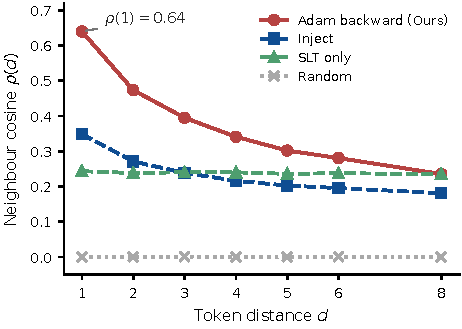
\includegraphics[width=\linewidth]{fig/figure/fig8a_spatial_decay.pdf}
    \caption{Measured spatial neighbour cosine $\rho(d)$ vs.\ token distance.
    Adam-backward updates are strongly coherent for neighbours ($\rho{=}0.64$)
    and stay coherent over distance; injection ($0.35$) is weaker, per-token SLT
    is flat-low ($0.24$, no local structure), and a random control is zero.}
    \label{fig:spatial_decay}
  \end{subfigure}\hfill
  \begin{subfigure}{0.48\textwidth}
    \centering
    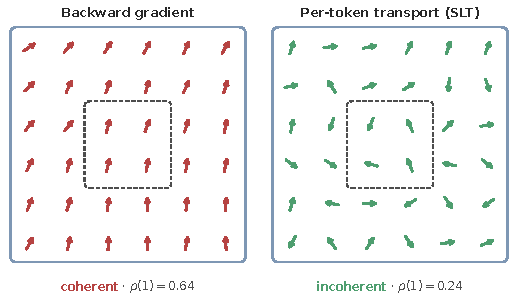
\includegraphics[width=\linewidth]{fig/figure/concept_spatial.pdf}
    \caption{Mechanism: the value-path self-attention Jacobian couples
    neighbouring tokens---adjacent content keys are nearly identical, so
    backpropagation delivers near-identical gradient directions to spatially
    adjacent positions, whereas per-token transport (SLT) has no such
    coupling ($\rho{=}0.24$; Table~\ref{tab:spatial_proof}).}
    \label{fig:concept_spatial}
  \end{subfigure}
  \caption{Spatial coherence of latent updates: \textbf{(a)} the
  \emph{measured} coherence $\rho(d)$ and \textbf{(b)} the value-path Jacobian
  \emph{mechanism} that produces it. Detailed per-token coherence maps
  are in the supplement (Fig.~\ref{fig:pca_maps}).}
  \label{fig:spatial_coherence}
\end{figure*}

% 十修: premise sentence rewritten for consistency with our own unified-protocol
% measurements (tab:percat, Sec.~\ref{sec:exp}), where the strongest trained
% baseline (CSGO) reaches only a mean CSD of 0.506; the 0.6--0.8 figure is what
% trained methods self-report under their own (non-unified) protocols.
Trained style methods produce coherent brushstroke texture, with
self-reported style fidelity of CSD~$\approx 0.6$--$0.8$ under their own
protocols; under our unified protocol the strongest baseline reaches only a
mean of $0.506$ (Table~\ref{tab:percat}).
To understand why, consider the gradient that flows back through the
self-attention module during fine-tuning.
Backpropagation couples tokens through the \emph{value path} of attention:
token $i$'s value contributes to the output at every position $j$ with
weight $A_{ji}$, so the gradient arriving at token $i$ aggregates residuals
from \emph{all} positions, weighted by the $i$-th column of the attention
matrix.
Neighboring tokens $(i,\,i{+}1)$ carry nearly identical keys—RoPE encodes
adjacent grid positions with nearly identical rotation
matrices~\cite{su2024rope} ($\|\mathbf{R}(\mathbf{p}_i){-}\mathbf{R}(\mathbf{p}_{i+1})\|_F
\approx 0.098$) and denoising latents are spatially smooth—so adjacent
attention columns nearly coincide and adjacent tokens receive nearly
identical gradient signals.
These correlated updates cause neighboring tokens to be nudged in the
\emph{same direction}, producing the long-range spatial correlations that
define painterly texture.

\paragraph{Empirical confirmation}
We measure this directly via the \emph{spatial neighbor cosine}:
\begin{equation}
  \rho = \frac{1}{|\mathcal{N}|} \sum_{(u,v) \in \mathcal{N}}
         \cos(\delta_{u},\, \delta_{v}),
  \label{eq:rho}
\end{equation}
where $\delta_{u}$ is the per-token latent update at grid position $u$ and
$\mathcal{N}$ is the set of horizontally and vertically adjacent position
pairs on the $32 \times 32$ token grid
($|\mathcal{N}| = 2 \times 31 \times 32$).
Results are shown in Table~\ref{tab:spatial_proof} and
Fig.~\ref{fig:spatial_coherence}a, with the convergence and gradient-source
analyses in Fig.~\ref{fig:spatial_proof}; the detailed per-token
update-direction coherence maps appear in the supplement
(Fig.~\ref{fig:pca_maps}).
Fig.~\ref{fig:spatial_proof}a shows that Backward$+$SLT (ours) converges
fastest, reaching at $N{=}2$ the style loss that backward-only optimization
requires $N{\approx}4$ to match, while the gradient-free Inject and SLT-only
baselines cannot iterate.
Fig.~\ref{fig:spatial_proof}b isolates the source of the coherence: shuffling
the spatial order of the style $K/V$ leaves $\rho$ unchanged ($0.654$ vs.\
$0.654$), ruling out the style-image layout; removing style $K/V$ entirely
collapses coherence to $\rho{=}0.168$, whereas a single-patch style loss
recovers most of it ($\rho{=}0.628$)---confirming that the self-attention
backward pass propagates the style signal globally through the value path.

\begin{figure}[tb]
  \centering
  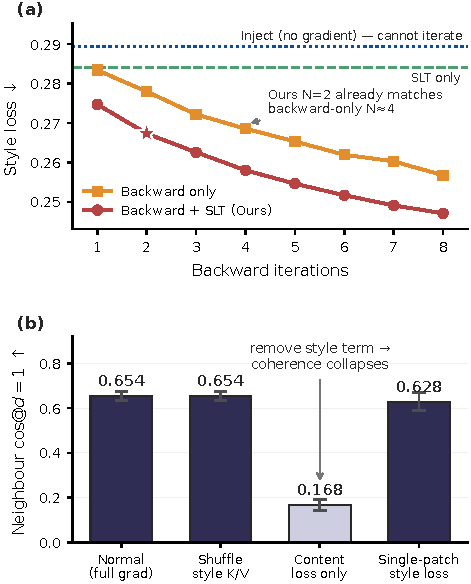
\includegraphics[width=\linewidth]{fig/figure/fig3_spatial_proof.pdf}
  \caption{Style-loss convergence (a) and the gradient-source analysis
  of spatial coherence (b); see Sec.~\ref{sec:method:gap}.}
  \label{fig:spatial_proof}
\end{figure}

\begin{table}[h]
  \centering
  \caption{Spatial neighbor cosine $\rho$ ($d{=}1$) by gradient source,
           measured at the first Adam iteration and averaged over 6
           content--style pairs (4 pairs for the content-loss-only and
           stop-grad-$Q$ conditions).
           Fig.~\ref{fig:spatial_proof}b visualizes the gradient-source
           conditions on the 4-pair ablation set (first iteration); minor
           value differences from this table reflect the smaller sample.
           Higher = more spatially coherent = brushstroke texture.}
  \label{tab:spatial_proof}
  \footnotesize
  \begin{tabular}{lcc}
    \toprule
    Gradient condition & $\rho$ & Interpretation \\
    \midrule
    Random direction (control)   & $0.00$  & No structure \\
    SLT per-token OT             & $0.24$  & Accidental proximity \\
    Content-loss-only gradient   & $0.17$  & Weak self-coupling \\
    Adam full gradient (backprop)& $0.64$  & \textbf{Value-path Jacobian} \\
    Stop-grad-$Q$ gradient       & $0.65$  & Value-path dominant \\
    \bottomrule
  \end{tabular}
\end{table}

The $2.6\times$ gap between Adam gradients ($\rho = 0.64$) and OT updates
($\rho = 0.24$) is the quantitative signature of the backpropagation gap:
training-free OT operates token by token independently, whereas backward-pass
gradients couple neighbors through the shared attention pattern and are
therefore $2.6\times$ more spatially coherent.

\begin{proposition}[Spatial gradient coherence]
\label{prop:spatial}
Let $g_i = \partial\mathcal{L}_\mathrm{style}/\partial z_i$ be the gradient of
the style-alignment loss at token $i$.
The content self-attention produces a \emph{value-path coupling term}
\begin{equation}
  g_i^{\mathrm{val}}
  = -2W_V \sum_{j} A_{ji}^c\, R_j,
  \label{eq:gval}
\end{equation}
where $A^c$ is the content attention matrix and $R = O_s - O_c$.
If content keys satisfy the $\epsilon$-spatial smoothness condition
$\|K_{c,i} - K_{c,i+1}\|_2 \leq \epsilon\sqrt{d}$ (with
$q_{\max}\epsilon \leq 1$, $q_{\max}$ the maximal query norm), then
\begin{equation}
  \cos\!\bigl(g_i^{\mathrm{val}},\, g_{i+1}^{\mathrm{val}}\bigr)
  \;\geq\; 1 - \tfrac{C\,\epsilon^2\|R\|_F^2}{\|g^{\mathrm{val}}\|_{\min}^2},
  \qquad C = 2e^2\|W_V\|_2^2\,q_{\max}^2\,L.
  \label{eq:prop1}
\end{equation}
SLT updates have $\partial\Delta_i/\partial z_j = 0$ for $i \neq j$ (with the
transport plan $T$ held fixed during the update, as in our implementation),
so no analogous coupling exists; their spatial coherence depends only on
accidental proximity of transport targets.
\end{proposition}

The key step (Appendix~\ref{app:jacobian}) is that $g_i^{\mathrm{val}}$
is a weighted average of the residual $R$ over \emph{all} positions, with
column weights $A_{ji}^c$ that are nearly equal for adjacent $i$ whenever
content keys are spatially smooth.
This smoothness is structurally motivated in MM-DiT~\cite{esser2024scaling}:
the RoPE rotation-difference bound~\cite{su2024rope}
$\|R(\mathbf{p}_i){-}R(\mathbf{p}_{i+1})\|_F \approx 0.098$ constrains the
positional part of the key difference $\|K_{c,i}{-}K_{c,i+1}\|$, and the
spatial smoothness of denoising latents constrains the remainder; the
resulting attention-weight difference is bounded by the softmax
logit-difference argument in Appendix~\ref{app:jacobian}.
SLT operates entirely in token-distribution space and bypasses the attention
Jacobian; $\partial\Delta_i/\partial z_j = 0$ for $i \neq j$ by construction,
which accounts for the $2.6\times$ gap in $\rho$.

\paragraph{Ablation --- which gradient path drives spatial coherence}
To isolate the value-path contribution experimentally, we compare three gradient
conditions: (i) \emph{Normal} (full gradient), (ii) \emph{Stop-grad-$Q$}
(Q detached before the attention product, removing the query-side gradient
path), and
(iii) \emph{Random direction} (control).
Normal and Stop-grad-$Q$ achieve identical spatial coherence
($\rho \approx 0.65$) at every iteration, while Random yields $\rho \approx 0.00$
(see Supplementary Fig.~\ref{fig:jacobian_ablation}).
The query-side Jacobian path is therefore \emph{not} the source of spatial
coherence; combined with the empirical subdominance of the key-side term
($\|g^K\|/\|g^{\mathrm{val}}\| < 0.15$, Appendix~\ref{app:jacobian}), this
identifies the value-path term $g_i^{\mathrm{val}}$ (Eq.~\ref{eq:gval}) as
the responsible mechanism, consistent with Proposition~\ref{prop:spatial}.

% ─────────────────────────────────────────────────────────────────────────────
\subsection{Adam-in-Loop Latent Optimization}
\label{sec:method:adam}

\begin{figure}[t]
  \centering
  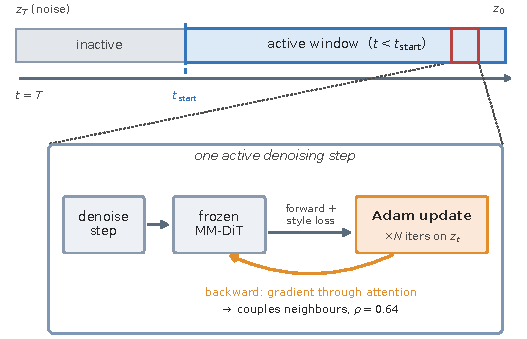
\includegraphics[width=\linewidth]{fig/figure/concept_adam.pdf}
  \caption{The Adam-in-loop schedule: $N$ Adam iterations inside each
  active denoising step ($t<t_\text{start}$).}
  \label{fig:concept_adam}
\end{figure}

The diagnosis suggests a direct fix: run backpropagation through the frozen
model at each denoising step, optimizing only the latent $z_t$.
No weights change; the gradient serves purely to propagate spatial coherence
into the latent update.
We call this \textbf{Adam-in-loop}. Fig.~\ref{fig:concept_adam} illustrates the schedule: at every active
step, gradients backpropagated through the frozen MM-DiT update the content
latent, supplying the cross-token spatial coupling.

\paragraph{Formulation}
At each denoising timestep $t < t_\text{start}$, after the standard denoising
update, we run $N$ Adam steps on a style-alignment loss:
\begin{multline}
  \mathcal{L}_\text{style} = \sum_{\ell}
  \bigl\|\text{Attn}(Q_c^{(\ell)}, K_s^{(\ell)}, V_s^{(\ell)}) \\
         - \text{Attn}(Q_c^{(\ell)}, K_c^{(\ell)}, V_c^{(\ell)})\bigr\|_1,
  \label{eq:adam_loss}
\end{multline}
with an $\ell_1$ content-anchor term to resist structural drift
($\mathcal{L} = w_s\mathcal{L}_\text{style} + w_c\mathcal{L}_\text{cnt}$,
$w_s{=}2.0$, $w_c{=}1.5$, lr$\,{=}\,0.03$).
Gradients flow through the content forward pass and through the
self-attention Jacobian, providing the spatial coherence that injection cannot.

% 十一修 评阅#6: 本小节原 \paragraph{Results}（迭代数-质量对照 + tab:iter_tradeoff
% 表 + Adam-8 保守配置选择规则）整体移入 Sec.4.5 Efficiency Analysis；第 3 节只留
% 原理与指针。
Iteration-count and equal-budget comparisons against Adam-only---and the
selection rule for the conservative Adam-8 reference configuration used in
Tables~\ref{tab:main} and~\ref{tab:ablation}---are analyzed in
Sec.~\ref{sec:exp:efficiency} (Table~\ref{tab:iter_tradeoff},
Fig.~\ref{fig:iter_tradeoff}).

% ─────────────────────────────────────────────────────────────────────────────
\subsection{Frequency-Domain Sinkhorn Loss}
\label{sec:method:freq}

\begin{figure}[t]
  \centering
  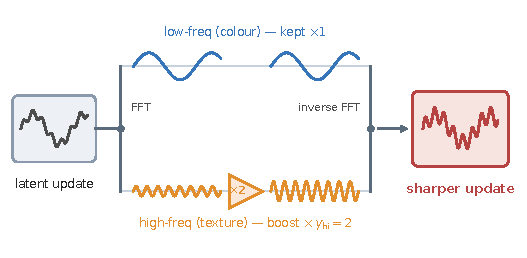
\includegraphics[width=\linewidth]{fig/figure/concept_freq.pdf}
  \caption{The frequency-domain Sinkhorn loss: the high-frequency band
  is amplified ($\gamma_\text{hi}{=}2$) before transport.}
  \label{fig:concept_freq}
\end{figure}

Before turning to Adam's efficiency bottleneck (Sec.~\ref{sec:method:slt}), we
describe one refinement internal to the style loss itself. Fig.~\ref{fig:concept_freq} sketches the mechanism: amplifying the
high-frequency (texture) band before transport sharpens brushstroke detail
without disturbing the global color alignment.
Within Adam's style loss $\mathcal{L}_\text{style}$, we decompose the latent
into low- and high-frequency components via per-channel frequency separation
and apply boosted transport weighting to the high-frequency component:
\begin{equation}
  \mathcal{L}_\text{style} = \mathcal{L}_\text{lo} + \gamma_\text{hi}\,\mathcal{L}_\text{hi},
  \quad \gamma_\text{hi} = 2.0.
  \label{eq:freq}
\end{equation}
The low-frequency component captures global tone; the high-frequency component
carries fine-grained texture: thin brushstrokes, sharp grain, edge details.
Standard $\ell_1$ loss, averaged over all frequency bands, under-weights
high-frequency terms because they carry less energy; the boost coefficient
$\gamma_\text{hi}=2.0$ corrects this, recovering fine-grained detail that
would otherwise be smoothed by the gradient averaging in Adam.
Ablation (Sec.~\ref{sec:ablation}) shows $+0.4\%$ CSD versus no boost.

% ─────────────────────────────────────────────────────────────────────────────
\subsection{Sinkhorn Latent Transport}
\label{sec:method:slt}

\begin{figure}[t]
  \centering
  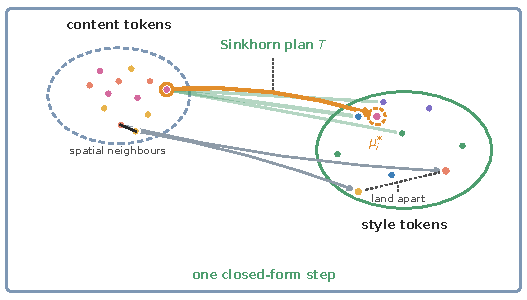
\includegraphics[width=\linewidth]{fig/figure/concept_slt.pdf}
  % 十一修(2026-07-06 评阅#3 二改): 图内三行说明文字删除，信息移入本 caption；
  % 图只保留六个短标签 + "one closed-form step" 一句 takeaway。
  \caption{Sinkhorn Latent Transport in the latent colour plane: the
  doubly-stochastic plan $T$ (green fan, line width $\propto T_{ij}$) matches
  each content token to the whole style distribution and moves it to its
  OT-weighted target $\mu^{*}_{i}$ in one closed-form AdaIN step
  ($\approx$0.1\,ms, no forward pass, no attention Jacobian). Adjacent tokens
  (solid link) are transported independently and land apart: colour is aligned
  but no cross-token coupling arises ($\rho(1){=}0.24$), hence no texture.}
  \label{fig:concept_slt}
\end{figure}

\paragraph{Gradient budget of early Adam iterations}
Profiling the Adam-in-loop gradient at each iteration reveals that the first
2--3 steps are dominated by the correction of low-frequency color mismatch
between $z_t$ and $z_s$.
Color distribution alignment is a global, per-channel operation that is
inefficient to perform via spatially local per-token gradient steps.
If this phase could be replaced by a single closed-form operation,
subsequent Adam iterations could begin immediately in the texture regime.

\paragraph{SLT formulation}
Optimal transport provides exactly this: the doubly-stochastic transport plan
$T = \text{Sinkhorn}(\tilde{S}/\tau)$ computed from the cosine-similarity matrix
$\tilde{S}_{ij} = \cos(\tilde{z}_t[i],\, \tilde{z}_s[j])$
over high-frequency residuals $\tilde{z} = z - \bar{z}$ (spatial mean subtracted)
globally matches each content token to a distribution over style tokens in a single
operation.
We use $T$ to derive per-token style distribution targets and apply
adaptive instance normalization~\cite{huang2017arbitrary}:
\begin{equation}
  \hat{z}_t[i] = \sigma^*_i\,\frac{z_t[i] - \mu_t}{\sigma_t} + \mu^*_i,
  \quad
  z_t \leftarrow (1-\alpha)\,z_t + \alpha\,\hat{z}_t,
  \label{eq:slt}
\end{equation}
where $\mu^*_i = \sum_j T_{ij}\,z_s[j]$ and $\sigma^*_i = \sqrt{\sum_j T_{ij}\,z_s[j]^2 - (\mu^*_i)^2}$
are the OT-weighted per-token target mean and standard deviation,
and $\mu_t, \sigma_t$ are the global statistics of the content latent
($\alpha{=}0.10$, $\tau{=}0.02$, $n_{\mathrm{iters}}{=}10$).
Compared to directly interpolating token embeddings
($z_t \leftarrow (1-\alpha)z_t + \alpha\,Tz_s$),
this OT-AdaIN formulation transfers per-token distribution statistics rather
than embedding values, preserving content structure while ensuring
global color alignment.
The doubly-stochastic constraint
($\sum_j T_{ij}{=}1$, $\sum_i T_{ij}{=}1$)
ensures every style token contributes to the transported statistics,
preventing the mode collapse that row-only softmax normalization permits.
The Sinkhorn solve runs in $\approx 0.1$~ms with no model forward pass;
the style features $z_s$ are already available from the attention injection
branch, so SLT adds zero additional forward passes. Fig.~\ref{fig:concept_slt} depicts the transport: it operates
directly in token space, bypassing the attention Jacobian---resolving color
cheaply while, by construction, producing no cross-token spatial coupling.

% 十一修 评阅#6: 原 \paragraph{SLT result and its limitation} 的实验数字
% （CSD 0.298 / ≈2.2s）移出——CSD 0.298 已由 Sec.5 的 "No Adam (SLT only)"
% 消融报告、wall-clock 已由 Sec.4.5 报告；本处只保留机制层面的局限性论述。
\paragraph{Structural limitation}
By construction the OT assignment is per-token independent: nothing
couples the update of token~$i$ to its neighbor's state, so SLT updates carry
low spatial coherence ($\rho = 0.24$, $2.6\times$ below Adam gradients;
Table~\ref{tab:spatial_proof}) and no spatially coherent structures emerge.
SLT resolves the global distribution gap but cannot generate \emph{local
structural correlations}; its measured quality ceiling and wall-clock cost are
quantified in the ablation (Sec.~\ref{sec:ablation}) and the efficiency
analysis (Sec.~\ref{sec:exp:efficiency}).

% ─────────────────────────────────────────────────────────────────────────────
\subsection{Layout Residual Suppression}
\label{sec:method:lrs}

Style K/V tensors carry both texture statistics and the spatial layout of the
reference image.
Injecting them unmodified causes content objects to drift toward reference
subject positions (\emph{layout leakage}).

\paragraph{Decomposition}
Any style key tensor decomposes as
$K_s^{(\ell)} = \mu_K^{(\ell)} + R_K^{(\ell)}$,
where $\mu_K^{(\ell)}$ is the token mean (permutation-invariant, carries
global style statistics) and $R_K^{(\ell)} = K_s - \mu_K$ is the
position-specific residual (carries spatial layout).

\paragraph{LRS suppression}
We attenuate the layout residual with a depth-dependent coefficient:
\begin{equation}
  K_s^{(\ell)\prime} = \mu_K^{(\ell)} + \gamma^{(\ell)}\,
                       (K_s^{(\ell)} - \mu_K^{(\ell)}),
  \label{eq:lrs}
\end{equation}
with the same transform applied to $V_s$; $\gamma^{(\ell)}$ is linearly
interpolated over block depth from $\gamma_\text{shallow}=0.7$ to
$\gamma_\text{deep}=0.5$.
Deeper blocks, whose features are more layout-specific, are attenuated more
strongly; the retained residual preserves texture directionality cues while
suppressing the layout leakage that causes subject-position drift.

\paragraph{Why this suppresses leakage}
Layout leakage arises because a content query $q_i$ attends to the style keys
with \emph{position-dependent} weights, importing \emph{where} the reference's
structures sit. Decompose the pre-softmax logit under \cref{eq:lrs}:
\begin{equation}
  q_i^\top K_{s,j}^{(\ell)\prime}
    \;=\; \underbrace{q_i^\top \mu_K^{(\ell)}}_{\text{constant in } j}
        \;+\; \gamma^{(\ell)}\, q_i^\top R_{K,j}^{(\ell)} .
  \label{eq:lrs_logit}
\end{equation}
The first term is identical for every style token $j$: it shifts all logits
equally and therefore \emph{cancels} in the softmax. Only the second,
position-varying term selects which style positions a token attends to, and its
dispersion across positions is scaled by $\gamma^2$:
\begin{equation}
  \operatorname{Var}_j\!\big(q_i^\top K_{s,j}^{(\ell)\prime}\big)
    \;=\; \big(\gamma^{(\ell)}\big)^2\,
          \operatorname{Var}_j\!\big(q_i^\top R_{K,j}^{(\ell)}\big).
  \label{eq:lrs_var}
\end{equation}
As $\gamma^{(\ell)}\!\to\!0$ the attention distribution over style tokens
becomes uniform: the output still draws on the global style statistics carried by
$\mu_K^{(\ell)}$ (palette, texture energy) but no longer on the \emph{spatial
arrangement} encoded in $R_K^{(\ell)}$, so the layout residual cannot propagate
into the generated image. As $\gamma^{(\ell)}\!\to\!1$ the full layout returns.
LRS therefore continuously trades layout leakage against texture retention, and
the depth schedule attenuates most strongly in the deep, layout-specific blocks
while preserving the shallow-block residual that carries brushstroke
directionality. Appendix~\ref{app:lrs_proof} makes the leakage bound precise.

% ─────────────────────────────────────────────────────────────────────────────
% ARCHITECTURE FIGURE
% ── IMAGE GENERATION PROMPT (vector diagram, export as PDF or high-res PNG) ─
%
%   Two-panel figure (top + bottom), see reference HTML: fig/architecture.html
%
%   TOP PANEL — Overall pipeline (horizontal flow):
%     Left: style branch
%       [x_s image icon] →[VAE (blue)]→ z_s →[Frozen Φ, dashed gray box]→ K_s,V_s →[LRS (green box)]→ K_s',V_s'
%     Center: denoising timeline
%       [p + z_T~N(0,I)] →───────────── ×25 denoising steps ─────────────→ z_0 →[VAE⁻¹]→ [output image]
%       Highlight active region (t < 850) with purple dashed rectangle; connect to bottom panel with bracket lines.
%     Style branch K_s',V_s' feeds down into the active region.
%
%   BOTTOM PANEL — Per-step module (horizontal flow, same color scheme):
%     z_t →[LRS block, green]→[SLT block, orange]→[Adam×2 block, red]→[Result box, purple] z_t'
%     LRS: "K_s' = μ_K + γ^(ℓ)·R_K  (γ^(ℓ): 0.7→0.5 by depth)"
%     SLT: "T=Sinkhorn(cos(z̃_t,z̃_s)/τ) · OT-AdaIN(z_t;T) · α=0.10 τ=0.02"
%          ρ badge: "ρ_SLT=0.24 (closes color gap, no J_attn)"
%     Adam×2: "∇_z L through J_attn · L=2.0L_sty+1.5L_cnt · freq-Sinkhorn boost γ_hi=2.0"
%             ρ badge: "ρ_Adam=0.64 → brushstrokes"
%             backprop curve arrow labeled "∂L/∂z_t"
%     Result: mini table (Inject <0.15 / SLT 0.298 / Adam-8 0.608 / Ours 0.640)
%             "+5.2% CSD vs Adam-8 · 2.5× lower fwd cost; +16.6% CSD at equal budget"
%
%   COLOR SCHEME: blue=style/frozen, green=LRS, orange=SLT, red=Adam, purple=contribution border
%   FONT: Helvetica/Arial 10–12pt, no serifs
%   EXPORT: fig/architecture.pdf at 300 dpi width ≥ 17cm (TPAMI double-column)
%   TOOL: Inkscape / draw.io / matplotlib + patches / TikZ
%   PREVIEW: fig/architecture.html (open in browser)
% ─────────────────────────────────────────────────────────────────────────────
% (framework overview figure moved to the Introduction as Fig.~\ref{fig:architecture})

% ─────────────────────────────────────────────────────────────────────────────
\subsection{Hyperion Pipeline: SLT Pre-Alignment with Adam Refinement}
\label{sec:method:hybrid}

\begin{figure*}[!t]
  \centering
  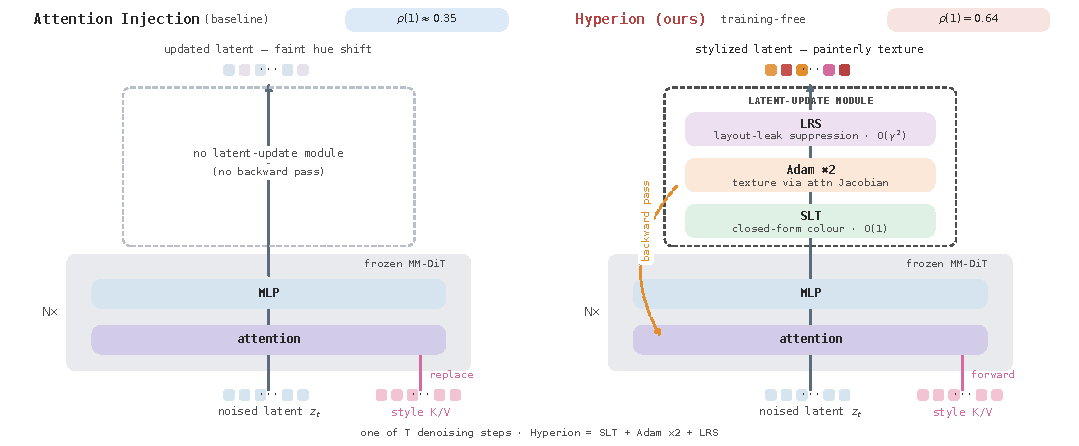
\includegraphics[width=\textwidth]{fig/figure/fig_framework_v4_pastel.pdf}
  \caption{One denoising step of the attention-injection baseline
  (left) and Hyperion (right); the two routes differ only in the
  latent-update module above the frozen backbone.}
  \label{fig:step_compare}
\end{figure*}

\paragraph{Design}
The two mechanisms are complementary with non-overlapping failure modes:
SLT is efficient at what Adam is slow at (global color alignment),
while Adam produces what SLT cannot (spatial texture coherence via the Jacobian).
The Hyperion pipeline (Fig.~\ref{fig:architecture}) chains them within each
denoising step in three stages.
Fig.~\ref{fig:step_compare} draws one such step next to the injection
baseline: the two routes differ only in whether the latent-update module fills
the lane above the frozen backbone.
Both panels share the same skeleton---the noised latent $z_t$ and the
style $K/V$ tokens enter the frozen MM-DiT---but injection applies no latent
update and yields only a faint hue shift ($\rho(1){\approx}0.35$), whereas the
chain SLT${\to}$Adam${\times}2{\to}$LRS produces spatially coherent texture
($\rho(1){=}0.64$).
First, the style branch supplies $K_s^{(\ell)}, V_s^{(\ell)}$ and LRS
layout-leakage suppression is applied (Sec.~\ref{sec:method:lrs}).
Second, the SLT pre-alignment (Eq.~\ref{eq:slt}, $\alpha=0.10$)
collapses the color distribution gap before Adam begins.
Third, two Adam steps are run on
$\mathcal{L} = 2.0\,\mathcal{L}_\text{style} + 1.5\,\mathcal{L}_\text{cnt}$
with frequency-domain Sinkhorn loss (Sec.~\ref{sec:method:freq}); because
the color gap is already closed, both iterations are spent entirely on texture,
generating brushstrokes through the Jacobian.
% 十修: disclose the two auxiliary AdaIN color operations (previously present
% in code but not in the algorithm/text); ablation numbers from the n=40
% color-mechanism decomposition (t2i_sltadam.csv: ota_a01 vs.\ ota_noAdain).
For completeness, we also disclose two auxiliary color operations that
bookend this loop, both applied unconditionally for Hyperion: a per-step
AdaIN warm-start toward the (noised) style latent statistics, applied right
after LRS and before SLT at every active step ($\alpha_w=0.5$); and a
terminal one-dimensional color correction applied once, after the denoising
loop, that matches the final latent's global per-channel statistics to those
of the (clean) style latent (Algorithm~\ref{alg:pipeline}). Removing both
costs only $0.683\!\to\!0.647$ CSD ($-0.036$) on the 40-sample ablation
subset, while CLIP-T is essentially unaffected (in fact rises slightly,
$0.274\!\to\!0.283$); the primary quality gain is therefore attributable to
SLT and Adam-in-loop rather than to these color-correction auxiliaries.

% 十修: A4 按作者意见保留主文定量界（审稿方案 b）——命题维持定量形式，
% 实测常数(κ≈0.67, δ≈1.6, cos≈0.26)直接印在正文 caveat 里而非仅指向附录，
% 使定量承诺与其适用域在同一页可见。命题本体恢复九修原文（非 \REV 项）。
\begin{proposition}[Pre-alignment iteration efficiency]
\label{prop:hybrid}
Decompose the style loss as $\mathcal{L} = \mathcal{L}_c + \mathcal{L}_t$
(color and texture components), with near-orthogonal gradients
$\langle g_c, g_t\rangle \approx 0$.
Assume (A1) $\|g_c(z^{(0)})\| \geq \kappa\|g(z^{(0)})\|$ with $\kappa \approx 0.85$,
(A2) $\|g_c(z^\mathrm{SLT})\| \leq \epsilon\|g(z^\mathrm{SLT})\|$ with $\epsilon \ll 1$,
and (A3) the SLT displacement changes $g_t$ by at most a relative
$\delta \ll 1$.
Model the optimizer as normalized gradient steps
$z^{+} = z - \eta\,g/\|g\|$ (the abstraction matching Adam's
magnitude-invariant step size).
Then, to first order in $\eta$, the per-step texture-loss decrease satisfies
\begin{align}
  \Delta_t^{H} &\geq \eta\,(1-2\epsilon-2\delta)\,\|g_t\|
  \quad\text{(Hyperion, at } z^\mathrm{SLT}\text{)}, \label{eq:hybrid_bound}\\
  \Delta_t^{A} &\leq \eta\,\sqrt{1-\kappa^2}\,\|g_t\|
  \quad\text{(pure Adam, at } z^{(0)}\text{)}, \label{eq:adam_bound}
\end{align}
so Hyperion's guaranteed texture progress per iteration exceeds the pure-Adam
ceiling by at least $(1-2\epsilon-2\delta)/\sqrt{1-\kappa^2} \approx
1.9\times$ in the idealized regime $\kappa = 0.85$, $\epsilon,\delta \ll 1$.
\end{proposition}

The intuition: a normalized optimizer spends a fixed step length per
iteration, and at $z^{(0)}$ the dominant color gradient consumes most of that
budget—the component of the step aligned with texture is at most
$\sqrt{1-\kappa^2} \approx 0.53$.
After SLT, $g_c \approx 0$, so essentially the entire step serves texture.
This $\approx 1.9\times$ per-step advantage is an idealized estimate: at
the directly profiled constants ($\kappa\approx0.67$, $\delta\approx1.6$,
gradient cosine $\approx0.26$; Appendix~\ref{app:hybrid},
Remark~\ref{rem:measured_constants}) the lower bound of
\cref{eq:hybrid_bound} is no longer positive, so the ratio should be read as
a mechanism statement about where the step budget goes rather than as a
pointwise numeric guarantee---but the empirical effect is unambiguous:
2 Hyperion iterations outperform 2 pure Adam iterations by $+16.6\%$ CSD on
the ablation subset.
The complete derivation is in Appendix~\ref{app:hybrid}.

% 十一修 评阅#6 追加（作者拍板）: 本小节原 \paragraph{Results} 同样移出——
% subset 头条数与 +16.6% 等预算对比并入 Sec.4.5（Equal-budget comparison 段）；
% 全基准 +5.2% 已由 Sec.4.2 承载、"Adam-only N≈4 才追平" 已由 Sec.4.5 既有
% operating-point 论述承载，删重不删数。
The complete pipeline is given in Algorithm~\ref{alg:pipeline};
headline comparisons on the full benchmark and the equal-budget
analysis appear in Secs.~\ref{sec:exp:main} and~\ref{sec:exp:efficiency}.

\begin{algorithm}[t]
  \caption{Hyperion Pipeline}  % 十一修 评阅#7: 改名（原 "Hyperion SLT + Adam style transfer"）
  \label{alg:pipeline}
  \begin{algorithmic}[1]
    \Require prompt $p$, style image $x_s$, frozen backbone $\Phi$
    \State $z_s \leftarrow \text{VAE}(x_s)$;\quad
           sample $z_T \sim \mathcal{N}(0,I)$
    \For{$t = T, T{-}1, \ldots, 1$}
      \State $z_t \leftarrow \text{denoise}(\Phi(z_t, t, p))$
      \If{$t < t_\text{start}$}\Comment{$t_\text{start}=850$ for T2I}
        \State $\{K_s^{(\ell)}, V_s^{(\ell)}\}
               \leftarrow \Phi\text{-fwd}(z_s^{(t)})$
        \State Apply LRS: $K_s^{(\ell)} \leftarrow
               \mu_K + \gamma^{(\ell)}(K_s^{(\ell)}-\mu_K)$
               \Comment{$\gamma^{(\ell)}$: $0.7 \to 0.5$ by depth}
        % 十修: AdaIN warm-start disclosed (was previously only in code,
        % eval_all.py:733-736); see Sec.~\ref{sec:method:hybrid} Design.
        \State AdaIN warm-start: $z_t \leftarrow (1{-}\alpha_w)\,z_t +
               \alpha_w\,\mathrm{AdaIN}(z_t,\, z_s^{(t)})$
               \Comment{$\alpha_w{=}0.5$, toward style stats}
        \State $T \leftarrow \text{Sinkhorn}(\cos(\tilde{z}_t, \tilde{z}_s)/\tau)$,
               $\tilde{z}{=}z{-}\bar{z}$
               \Comment{$\tau{=}0.02$, 10~iters}
        \State $z_t \leftarrow$ OT-AdaIN$(z_t, z_s;\, T,\, \alpha{=}0.10)$
               \Comment{Eq.~\ref{eq:slt}}
        \For{$n = 1, 2$}
          \State forward $\Phi(z_t)\to Q_c$, compute $\mathcal{L}$
                 \Comment{freq-domain Sinkhorn loss}
          \State $z_t \leftarrow \mathrm{AdamStep}\bigl(z_t,\,
                 \nabla_{z_t}\mathcal{L}\bigr)$
                 \Comment{lr$\,{=}\,0.03$}
        \EndFor
      \EndIf
    \EndFor
    % 十修: terminal color correction disclosed (was previously only in code,
    % eval_all.py:852-854); gated off for the text-only/raw-injection
    % baselines, on by default for Hyperion.
    \State $z_0 \leftarrow \mathrm{AdaIN}_{1D}(z_0,\, z_s)$
           \Comment{terminal color correction, gated on for Hyperion}
    \State \Return $\text{VAE}^{-1}(z_0)$
  \end{algorithmic}
\end{algorithm}

% ─────────────────────────────────────────────────────────────────────────────
\subsection{Extension to Image-to-Image Style Transfer}
\label{sec:method:i2i}

% 2026-07-03 八修: fig:concept_i2i retired at the author's direction (its
% mechanism drawing is under review, HUMAN_REVIEW_NEEDED.md #A3, and it was
% never \ref'd); the slot is taken by fig:step_compare (figure* hung at
% sec:method:hybrid). The old fig/figure/concept_i2i.pdf + TikZ source and
% dossier are kept for the #A3 decision.
% 十修: corrected mechanism description — the previous "content-init AdaIN"
% paragraph below had the AdaIN direction reversed relative to the code (the
% only AdaIN call in generate_i2i, eval_all.py:1026-1029, warms the noised
% *style* latent, identically to T2I, just at a lower alpha; it never targets
% content statistics). The true content-conditioning mechanism is in-context
% token concatenation (eval_all.py:887-904,954-961), disclosed below.
The T2I Hyperion pipeline extends to image-conditioned (I2I) inputs with
three modifications; all other components (SLT, Adam, LRS, freq-boost)
are unchanged. (i) the content image conditions the denoising process
via in-context token concatenation rather than latent initialization; (ii)
the per-step AdaIN warm-start of Algorithm~\ref{alg:pipeline} is reused
unchanged in form, with $\alpha_w$ lowered from $0.5$ to $0.3$; and (iii) the
injection start time is shifted from $t_\text{start}=850$ to $870$.

\paragraph{Content conditioning via in-context tokens}
As in T2I, the initial latent $z_T$ is pure Gaussian noise with no
structural prior; the content image instead enters as in-context
conditioning rather than as a latent initialization. We encode
$z_c = \text{VAE}(x_c)$ once and, at every denoising step, concatenate it to
the denoising latent along the token axis before the forward pass, assigning
it distinct positional ids from the image latent's own; only the $L$-token
prefix of the model's output is kept for the update:
\begin{equation}
  \hat{v}_t = \Phi\bigl(\operatorname{concat}(z_t,\, z_c),\, t,\, p\bigr)[:L],
  \label{eq:adain}
\end{equation}
% 十修: eq:adain now documents the true I2I content-conditioning mechanism
% (in-context token concatenation); label kept unchanged since nothing in the
% repo \ref's it (grep -rn "eq:adain" turns up only this \label).
where $L$ is the token length of $z_t$ and $[:L]$ truncates the model's
per-token prediction to the image-latent prefix, discarding the prediction
at the content-token positions. Crucially, $z_c$ itself is never denoised and
never mixed into the statistics of $z_t$: the content image's structure
reaches the output only through the attention that $z_t$'s tokens pay to the
$z_c$ tokens at every forward pass, not through any modification of $z_t$'s
initial distribution or per-channel statistics. This concatenation runs at
every denoising step unconditionally, independent of $t_\text{start}$.

\paragraph{Re-weighted style warm-start and start time}
The per-step AdaIN warm-start toward the (noised) style latent
statistics introduced in Algorithm~\ref{alg:pipeline} is reused unchanged in
form for I2I; only its strength is lowered, $\alpha_w\!: 0.5 \to 0.3$, since
with content structure already supplied at every step by the in-context
tokens above, a weaker color pre-set suffices before SLT begins.
The T2I start time $t_\text{start}=850$ is calibrated for noise-initialized
latents, where 25 steps of denoising from pure noise are needed before
semantic structure is coherent enough for style injection.
For I2I, structural content is already available to every denoising
step through the concatenated tokens described above---rather than being
encoded in the initial latent---so meaningful content features are present
one step earlier; we set $t_\text{start}=870$ (one additional step) to
exploit this, giving the content branch a one-step head-start against the
style signal.
All other hyperparameters ($\alpha{=}0.10$, $\tau{=}0.02$, $N{=}2$,
$\gamma_\text{hi}{=}2.0$, $\gamma^{(\ell)}{=}0.7{\to}0.5$) are unchanged.

\section{Experiments}
\label{sec:exp}

% ─────────────────────────────────────────────────────────────────────────────
\subsection{Experimental Setup}
\label{sec:exp:setup}

\paragraph{Model and hardware}
All experiments use Klein~9B (MM-DiT architecture, 8 double-stream + 24
single-stream blocks, 32 layers total) via the DiffSynth backend, run in
bf16 mixed precision on a single H200 GPU.
Outputs are generated at $512 \times 512$ resolution with 25 denoising steps,
guidance scale~3.5, and fixed seed~43.
No model parameters are modified.

\paragraph{Benchmark construction}
We assemble a benchmark of 40 style references
(\texttt{sty/00}--\texttt{sty/39}) curated to span the breadth of visual styles a
training-free method must handle: traditional media (oil impasto, watercolor, ink
line art, bronze relief, ukiyo-e), graphic and illustrative styles (flat-color
posters, screenprint, art-deco, constructivist propaganda, comic), digital and
pixel art, and photographic textures. References were chosen for mutual visual
distinctness so that style fidelity is not inflated by near-duplicate references.
We exclude \texttt{sty04} from all T2I evaluation because its near-uniform pixel
statistics make the CSD embedding degenerate, leaving 39 styles.
% 十修: 删除过期表述"I2I additionally excludes sty14 and content cnt19 as
% pathological edge cases"——与事实矛盾: I2I 消融子集的 8 风格
% (00/10/14/20/27/28/33/38) 本身即含 sty14 (见下方 Evaluation splits 段)，
% 完整 741-pair I2I benchmark (39 styles x 19 contents, 见本文件 "full
% 741-pair I2I benchmark" 处) 同样不排除 sty14，且 cnt19 不存在于 19 个
% content 编号 (00--18) 范围内。该句为旧协议残留，予以删除。
The
six T2I content prompts (Table~\ref{tab:prompts}) are fixed in advance to span
object, animal, still-life, landscape, and architectural categories, decoupling
measured style fidelity from any single content type. The full style bank is
shown in the supplement (Fig.~\ref{fig:benchmark_atlas}).

\paragraph{Evaluation splits}
\emph{T2I} pairs every retained style with all six prompts
($39 \times 6 = 234$ pairs). \emph{Ablations and sweeps} use a 40-sample
subset---8 styles (\texttt{sty} 00/10/14/20/27/28/33/38) $\times$ 5 prompts
(\texttt{kp0}--\texttt{kp4})---chosen to span the style categories above while
permitting rapid iteration; the multi-seed robustness study reuses this subset.
\emph{I2I} uses a 40-pair subset: the same 8 styles $\times$ 5 content images
(\texttt{cnt} 00/04/08/12/17).

\begin{table}[h]
  \centering
  \caption{T2I benchmark content prompts.}
  \label{tab:prompts}
  \small
  \begin{tabular}{ll}
    \toprule
    ID & Prompt \\
    \midrule
    p0 & A cat sitting on a wooden table \\
    p1 & A sports car on a mountain road \\
    p2 & A field of sunflowers at sunset \\
    p3 & A dog running in a park \\
    p4 & A snowy mountain peak at dawn \\
    p5 & Portrait of a young woman \\
    \bottomrule
  \end{tabular}
\end{table}

\paragraph{Metrics}
We report three metrics, uniformly applied across all experiments.
\textbf{CSD}~($\uparrow$), the Contrastive Style Descriptor
similarity~\cite{somepalli2024measuring} between output and style reference,
serves as the primary style-fidelity metric.
\textbf{CLIP-T}~($\uparrow$), the CLIP ViT-B/32~\cite{radford2021learning}
image-text cosine similarity between output and content prompt,
measures content preservation.
\textbf{Forward passes / step}~($\downarrow$) counts the number of model forward
passes per denoising step, a hardware-agnostic efficiency metric; wall-clock
timing (each Adam iteration—one forward plus one backward pass per denoising
step—adds $\approx$2.1~s to total generation time on H200) is provided as
informational reference only, as absolute values depend on GPU load.
For I2I evaluation we additionally report \textbf{CLIP-I}~($\uparrow$)~\cite{radford2021learning}:
CLIP image-embedding cosine similarity between output and content image.

\paragraph{Baselines}
We evaluate two training-free \emph{floor} baselines directly.
\textbf{Text-only} runs standard inference with no style injection and serves as
the lower bound on style fidelity.
\textbf{Inject} applies single-step attention injection per
\cref{eq:injection} with $\beta=0.5$, a near-zero-cost
attention-replacement reference.
We additionally position our method against three training-free MM-DiT
competitors---\textbf{StyleAligned}~\cite{hertz2024style} (self-attention K/V
sharing), \textbf{V-Shuffle}~\cite{vshuffle2025} (stochastic value-token
permutation), and \textbf{Inversion-Free Dual RF}~\cite{dualrf2025} (dual
rectified-flow cross-branch injection, the closest competitor on MM-DiT).
Lacking public Klein~9B implementations of these three, we discuss them
qualitatively and benchmark quantitatively against four \emph{trained} style
adapters (StyleShot, USO, CSGO, IP-Adapter) across 21 diverse style families
(Sec.~\ref{app:trained_baselines}).

% ─────────────────────────────────────────────────────────────────────────────
\subsection{Main Comparison}
\label{sec:exp:main}

Table~\ref{tab:main} reports results on the full T2I benchmark
($39 \times 6 = 234$ pairs).

\begin{table}[t]
  \centering
  \caption{%
    T2I style transfer comparison on the full benchmark (39 styles $\times$ 6 prompts).
    Forward passes / step reported as the computational cost metric;
    wall-clock timing in parentheses is indicative (single H200, seed 43).
    STM is the Style--Texture Match (Sec.~\ref{sec:exp:texcoh}); it climbs
    monotonically with style-transfer strength and peaks for Hyperion.
    Text-only and Inject are training-free floor references measured on the
    40-sample subset (STM for Text-only/Inject/SLT-only likewise on the subset).%
  }
  \label{tab:main}
  \begin{tabular}{lcccc}
    \toprule
    Method & CSD~$\uparrow$ & CLIP-T~$\uparrow$ & STM~$\uparrow$ & Fwd./step \\
    \midrule
    Text-only                & $-0.01$ & 0.315   & 0.350 & 1 \\
    Inject                   & 0.039   & 0.314   & 0.395 & 2 \\
    \midrule
    Adam-8 (no SLT)                & 0.608   & 0.279   & 0.726 & 10 \\
    SLT only (no Adam)             & 0.298   & 0.309   & 0.624 & 2  \\
    \rowcolor{tabshade!10}
    \textbf{Ours (Hyperion)}         & \textbf{0.640} & 0.296 & \textbf{0.775} & 4 \\
    \bottomrule
  \end{tabular}
\end{table}

The Hyperion method achieves CSD~$= 0.640$ with only 4 forward passes per step
($2.5\times$ fewer than Adam-8) while exceeding Adam-8's CSD by \textbf{+5.2\%}.
Repeating the full benchmark across three seeds $\{43, 44, 45\}$ gives
CSD~$= 0.638 \pm 0.004$ (Hyperion) and $0.608 \pm 0.007$ (Adam-8); the
non-overlapping intervals confirm the advantage is seed-robust (the table
reports seed~43).
The Adam-8 row uses the conservative configuration
whose selection rule is given in Sec.~\ref{sec:exp:efficiency}
(lr$\,{=}\,0.01$, $w_c{=}0.2$).  % 十一修: 原指向 sec:method:adam，选择规则已随 #6 移入 4.5
SLT alone achieves CSD~$= 0.298$ at minimum cost but produces no brushstroke
texture; the spatial neighbor cosine analysis in Sec.~\ref{sec:method:gap}
explains why.
Against trained style adapters (StyleShot, USO, CSGO, IP-Adapter), Hyperion
attains higher style fidelity on 19 of 21 diverse-style families despite being
training-free (per-family CSD in Table~\ref{tab:percat};
qualitative comparison in Fig.~\ref{fig:diverse_main}).

\paragraph{Comparison to training-free value manipulation}
The closest training-free competitors---StyleAligned~\cite{hertz2024style},
V-Shuffle~\cite{vshuffle2025}, and Inversion-Free Dual~RF~\cite{dualrf2025}---were
built for SDXL/rectified-flow backbones and have no public MM-DiT release.
To compare directly rather than omit them, we implement a faithful MM-DiT
adaptation of V-Shuffle, the representative value-manipulation method (style
keys injected, style values spatially permuted, standard attention; two forward
passes, no backward), and evaluate it on the identical 234-pair Klein-9B
benchmark.
V-Shuffle reaches only CSD~$=0.232$---far below our $0.640$ (paired
$t{=}{+}47.9$, $p<10^{-100}$; our CSD is higher on \emph{all} $234/234$ pairs)---and
it also trails on prompt alignment (CLIP-T~$=0.230$ vs.\ our $0.296$;
$t{=}{+}16.5$).
On the Klein-9B MM-DiT, spatially permuting the style values severs the
style--content correspondence and transfers \emph{incoherent} texture rather than
coherent brushstroke style (Fig.~\ref{fig:vshuffle_cmp}): our SLT$+$Adam pipeline
therefore \emph{dominates} it on both style fidelity and prompt adherence.
This corroborates our central claim---coherent style requires the cross-token
coupling of a backward pass, which value-shuffling injection lacks.

\paragraph{Qualitative results}
Injection-based methods (\textit{inject}, StyleAligned) produce faint
hue shifts; V-Shuffle instead over-transfers texture at the expense of content
(see below); Adam-8 generates brushstrokes but over-stylizes some content;
Ours achieves rich texture with clear subject preservation.
SLT-only outputs show good color fidelity but plainly lack local texture.
Fig.~\ref{fig:diverse_main} compares our training-free Hyperion against four
trained adapters---StyleShot~\cite{gao2024styleshot}, USO~\cite{wu2025uso},
CSGO~\cite{xing2024csgo}, IP-Adapter~\cite{ipadapter2023}---across eight
maximally distinct style families (line/ink, ink-wash, 3D/sculptural,
pixel, textile/craft, geometric, flat-illustration, print/poster).
% 十一修: 主图第二行 27 Oil impasto -> 08 Chinese ink（用户指示），类别词
% painterly->ink-wash、结构词 palette-knife facets->graded ink washes 同步。
Ours reproduces the medium-defining structure---gouged relief, graded
ink washes, embossed metal, blocky dithering, square tesserae, polygonal
planes, hard-edge color blocks, dense ink hatching---where trained adapters
more often settle for color-only shifts or partial medium match. A per-family CSD breakdown
across 21 diverse media
(Table~\ref{tab:percat}) confirms the trend quantitatively: our
training-free method leads on \textbf{19 of 21} families (mean CSD $0.657$ vs.\
$0.506$ CSGO, $0.489$ StyleShot, $0.454$ USO, $0.420$ IP-Adapter).
% 十一修: 38/01 两行改为人工目选种子（47/46），披露句相应改为"按行选自 6 种子"，
% 不再声称全部由 CSD/CLIP-T 联合分选出。
The Hyperion tiles displayed in Fig.~\ref{fig:diverse_main} are
per-style selections from six seeds $\{43\text{--}48\}$ (chosen for the
clearest medium rendition); all quantitative tables use the fixed seed~43.

\begin{figure*}[!tp]
  \centering
  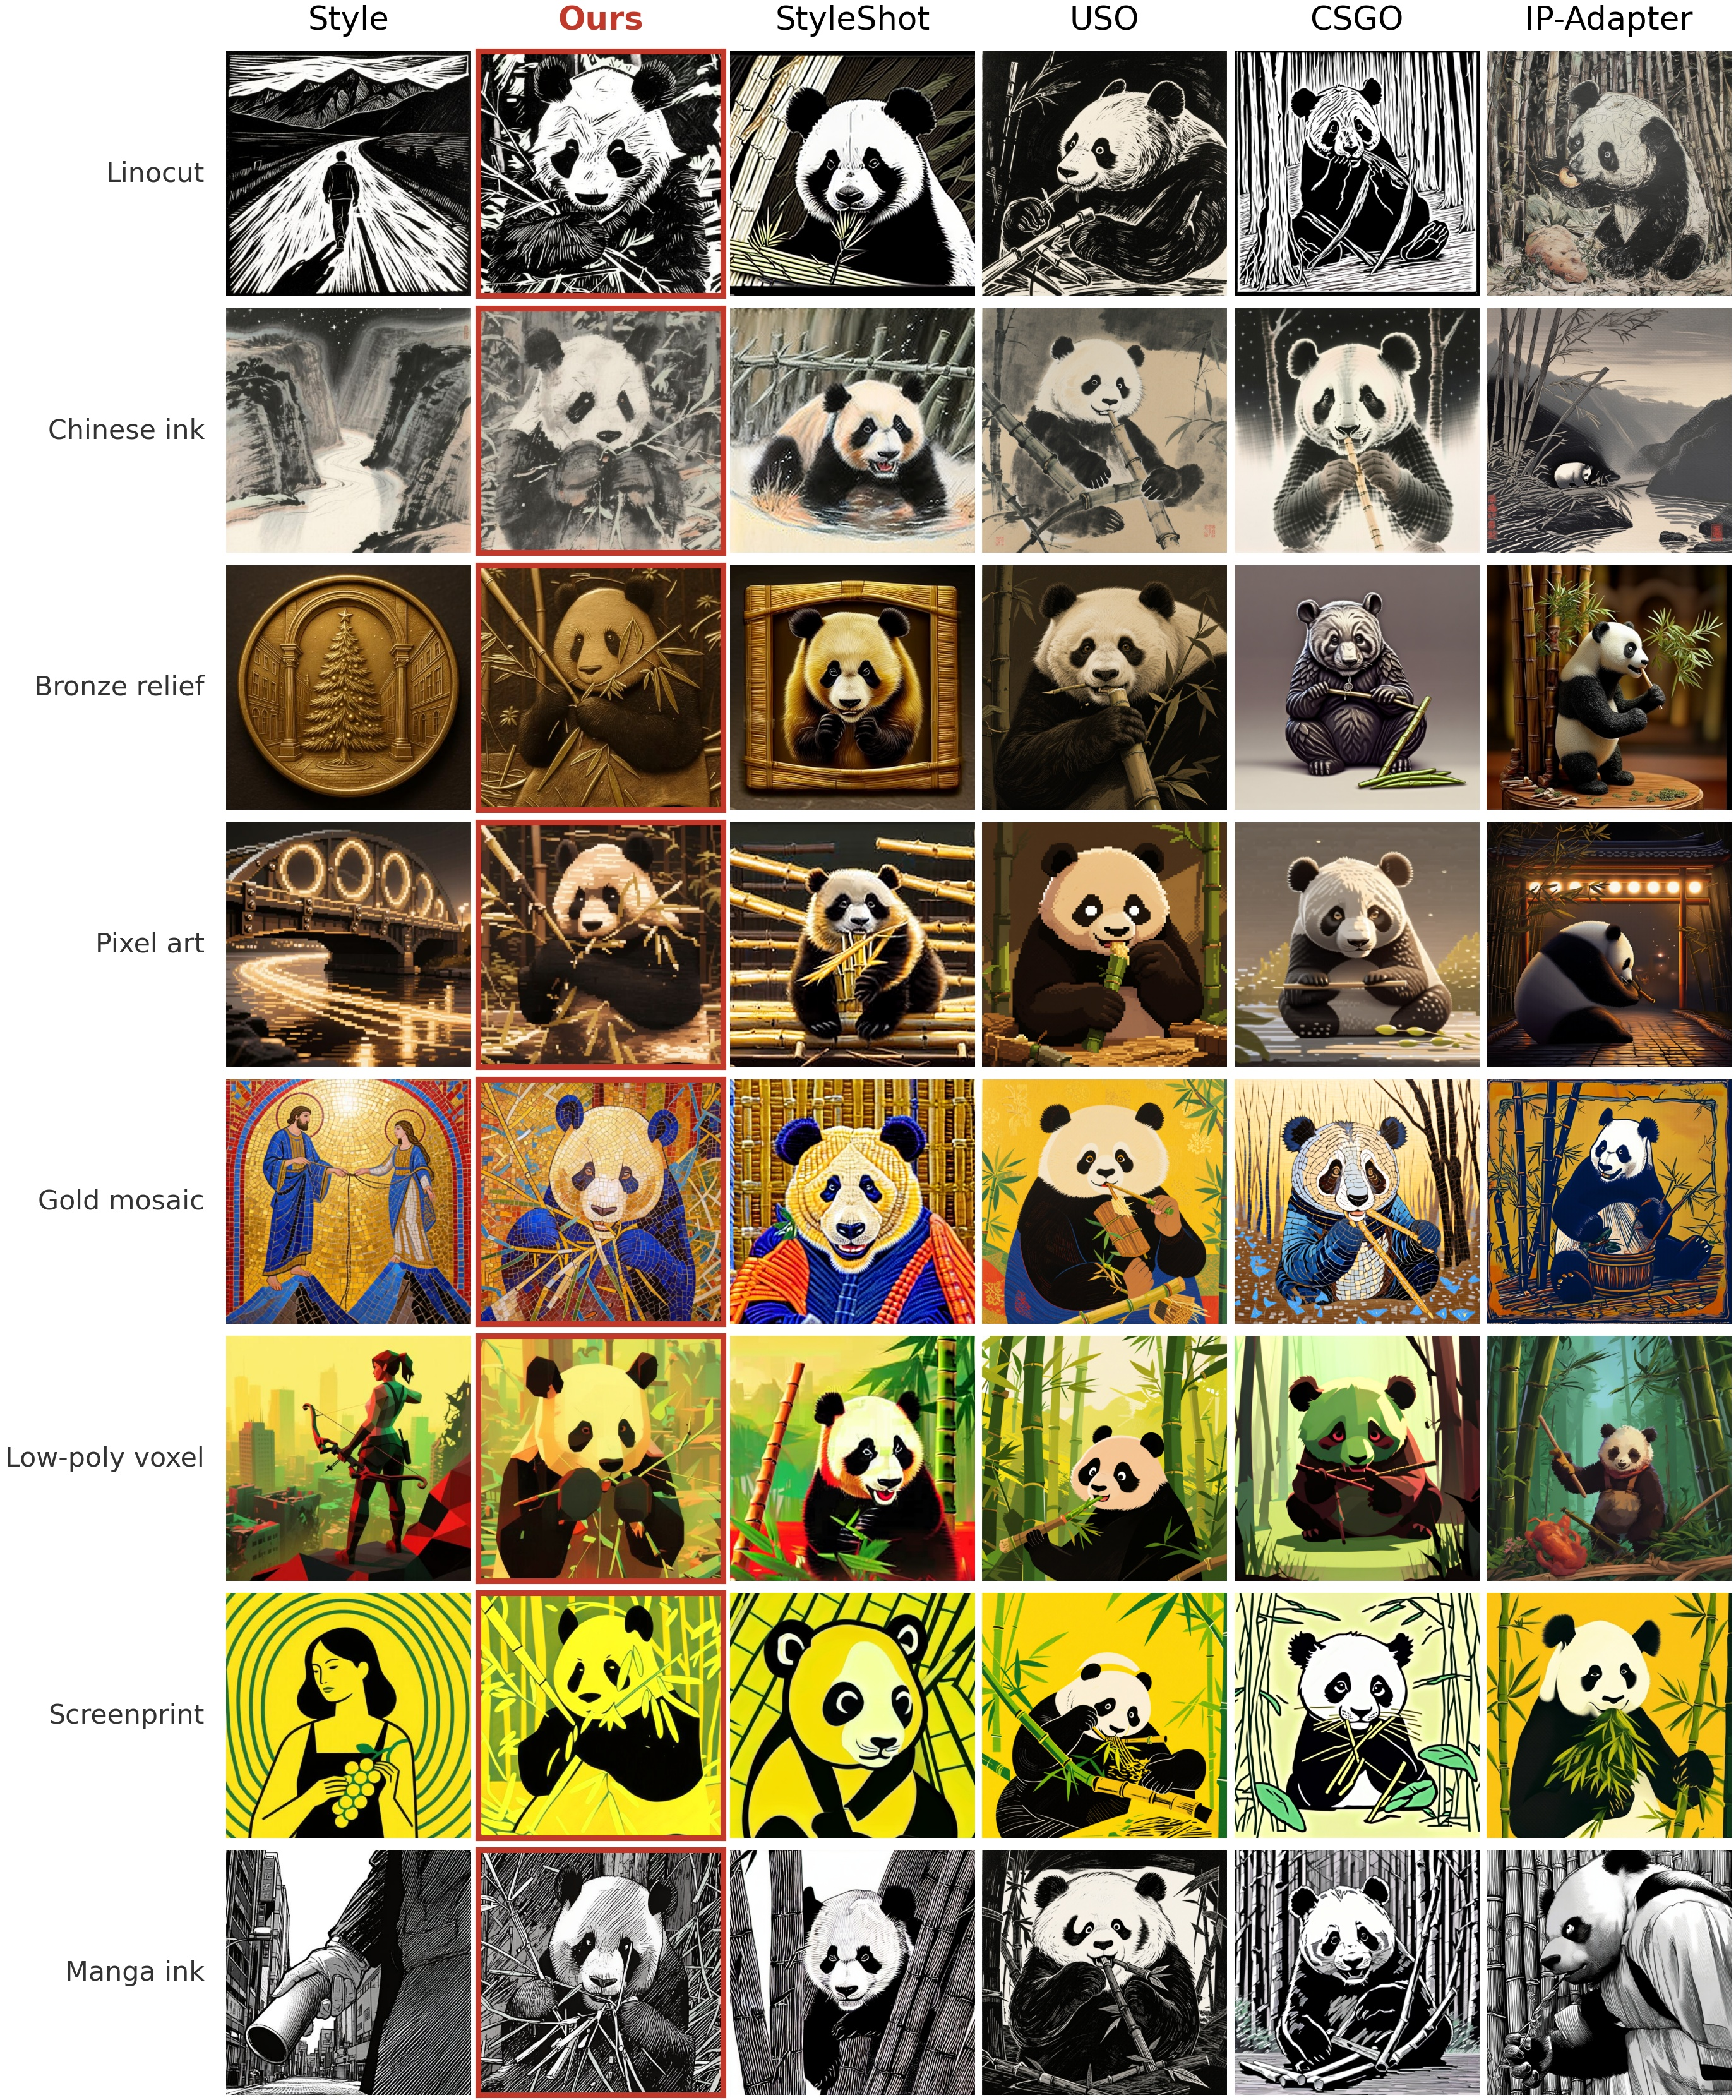
\includegraphics[width=.98\linewidth]{fig/figure/fig15_diverse_main.jpg}
  \caption{Qualitative comparison with four trained adapters across
    eight maximally distinct style families (prompt: ``A panda eat bamboo'');
    columns: style reference, Ours (Hyperion), StyleShot, USO, CSGO,
    IP-Adapter. Best viewed zoomed.}
  \label{fig:diverse_main}
\end{figure*}

\begin{table}[t]
  \centering
  % 十修: dropped stale "(prompt ``A panda eat bamboo'')" — that is the prompt of
  % the qualitative fig:diverse_main only; this table is a multi-prompt mean
  % (Ours: 6 prompts, baselines: 5), as now disclosed at the caption end.
  % 十修: Ours column recomputed as a 5-prompt mean (p0-p4, dropping p5) to match
  % the baselines' prompt set, from results/t2i_full_benchmark.csv
  % (method=hybrid2). Zero win/loss flips vs. the prior 6-prompt values
  % (still 19/21); shading P recomputed per-cell with the same formula below;
  % Mean 0.655 -> 0.657.
  \caption{Per-style-family CSD ($\uparrow$) across 21 diverse style media
  (mean over content prompts). Best per row in
  \textbf{bold}; cell shading encodes the CSD value on a single scale
  across the whole table (darker = higher). Our training-free Hyperion leads on
  19/21 families; the two
  exceptions (manga, anime) go to IP-Adapter, which is tuned for character imagery.
  Ours is recomputed from the full seed-43 benchmark over the 5 prompts
  shared with the baselines (p0--p4); trained baselines are run at their
  native resolution (Sec.~\ref{app:trained_baselines}).}
  \label{tab:percat}
  \footnotesize
  \setlength{\tabcolsep}{4.5pt}
  \begin{tabular}{l ccccc}
  \toprule
  Style family & Ours & StyleShot & USO & CSGO & IP-Ad. \\
  \midrule
  % cell shading: P = (v-0.154)/(0.779-0.154)*55, one scale for the whole table
  Pop halftone     & \cellcolor{tabshade!43}\textbf{0.644} & \cellcolor{tabshade!37}0.580 & \cellcolor{tabshade!24}0.432 & \cellcolor{tabshade!18}0.363 & \cellcolor{tabshade!3}0.190 \\
  Screenprint      & \cellcolor{tabshade!47}\textbf{0.686} & \cellcolor{tabshade!41}0.616 & \cellcolor{tabshade!40}0.603 & \cellcolor{tabshade!27}0.463 & \cellcolor{tabshade!34}0.536 \\
  Ink storybook    & \cellcolor{tabshade!33}\textbf{0.530} & \cellcolor{tabshade!17}0.346 & \cellcolor{tabshade!17}0.349 & \cellcolor{tabshade!28}0.473 & \cellcolor{tabshade!32}0.515 \\
  Bronze relief    & \cellcolor{tabshade!38}\textbf{0.588} & \cellcolor{tabshade!23}0.421 & \cellcolor{tabshade!0}0.154 & \cellcolor{tabshade!5}0.206 & \cellcolor{tabshade!15}0.322 \\
  Impasto collage  & \cellcolor{tabshade!47}\textbf{0.683} & \cellcolor{tabshade!27}0.464 & \cellcolor{tabshade!36}0.565 & \cellcolor{tabshade!34}0.544 & \cellcolor{tabshade!10}0.266 \\
  Embroidery       & \cellcolor{tabshade!49}\textbf{0.709} & \cellcolor{tabshade!33}0.526 & \cellcolor{tabshade!28}0.472 & \cellcolor{tabshade!45}0.668 & \cellcolor{tabshade!15}0.321 \\
  Linocut          & \cellcolor{tabshade!46}\textbf{0.672} & \cellcolor{tabshade!29}0.489 & \cellcolor{tabshade!36}0.559 & \cellcolor{tabshade!39}0.597 & \cellcolor{tabshade!9}0.259 \\
  Manga ink        & \cellcolor{tabshade!40}0.611 & \cellcolor{tabshade!24}0.428 & \cellcolor{tabshade!18}0.364 & \cellcolor{tabshade!35}0.550 & \cellcolor{tabshade!41}\textbf{0.622} \\
  Gold mosaic      & \cellcolor{tabshade!36}\textbf{0.558} & \cellcolor{tabshade!24}0.430 & \cellcolor{tabshade!10}0.267 & \cellcolor{tabshade!28}0.470 & \cellcolor{tabshade!8}0.246 \\
  Oil impasto      & \cellcolor{tabshade!49}\textbf{0.713} & \cellcolor{tabshade!35}0.553 & \cellcolor{tabshade!35}0.547 & \cellcolor{tabshade!43}0.639 & \cellcolor{tabshade!8}0.243 \\
  Blue screenprint & \cellcolor{tabshade!53}\textbf{0.751} & \cellcolor{tabshade!28}0.467 & \cellcolor{tabshade!33}0.527 & \cellcolor{tabshade!34}0.546 & \cellcolor{tabshade!34}0.539 \\
  Pixel art        & \cellcolor{tabshade!44}\textbf{0.656} & \cellcolor{tabshade!12}0.289 & \cellcolor{tabshade!23}0.411 & \cellcolor{tabshade!32}0.512 & \cellcolor{tabshade!26}0.448 \\
  Propaganda       & \cellcolor{tabshade!43}\textbf{0.645} & \cellcolor{tabshade!35}0.550 & \cellcolor{tabshade!26}0.455 & \cellcolor{tabshade!24}0.432 & \cellcolor{tabshade!6}0.220 \\
  Low-poly voxel   & \cellcolor{tabshade!51}\textbf{0.730} & \cellcolor{tabshade!42}0.633 & \cellcolor{tabshade!28}0.476 & \cellcolor{tabshade!46}0.672 & \cellcolor{tabshade!21}0.392 \\
  \midrule \multicolumn{6}{l}{\textit{Extended iconic families}}\\
  Anime cel        & \cellcolor{tabshade!44}0.654 & \cellcolor{tabshade!27}0.464 & \cellcolor{tabshade!25}0.442 & \cellcolor{tabshade!26}0.455 & \cellcolor{tabshade!48}\textbf{0.703} \\
  Chinese ink      & \cellcolor{tabshade!41}\textbf{0.618} & \cellcolor{tabshade!11}0.281 & \cellcolor{tabshade!29}0.489 & \cellcolor{tabshade!27}0.466 & \cellcolor{tabshade!32}0.516 \\
  Cyberpunk neon   & \cellcolor{tabshade!55}\textbf{0.782} & \cellcolor{tabshade!42}0.636 & \cellcolor{tabshade!37}0.575 & \cellcolor{tabshade!41}0.615 & \cellcolor{tabshade!41}0.616 \\
  Graffiti         & \cellcolor{tabshade!46}\textbf{0.678} & \cellcolor{tabshade!38}0.591 & \cellcolor{tabshade!14}0.318 & \cellcolor{tabshade!26}0.455 & \cellcolor{tabshade!19}0.366 \\
  Stained glass    & \cellcolor{tabshade!43}\textbf{0.638} & \cellcolor{tabshade!34}0.542 & \cellcolor{tabshade!31}0.503 & \cellcolor{tabshade!32}0.518 & \cellcolor{tabshade!30}0.492 \\
  Steampunk        & \cellcolor{tabshade!43}\textbf{0.640} & \cellcolor{tabshade!35}0.556 & \cellcolor{tabshade!31}0.504 & \cellcolor{tabshade!27}0.461 & \cellcolor{tabshade!30}0.499 \\
  Ukiyo-e          & \cellcolor{tabshade!41}\textbf{0.616} & \cellcolor{tabshade!23}0.416 & \cellcolor{tabshade!32}0.522 & \cellcolor{tabshade!33}0.527 & \cellcolor{tabshade!30}0.500 \\
  \midrule
  \textbf{Mean}    & \cellcolor{tabshade!44}\textbf{0.657} & \cellcolor{tabshade!29}0.489 & \cellcolor{tabshade!26}0.454 & \cellcolor{tabshade!31}0.506 & \cellcolor{tabshade!23}0.420 \\
  \midrule
  STM (mean)       & \textbf{0.738} & 0.695 & 0.405 & 0.567 & 0.569 \\
  \bottomrule
  \end{tabular}
\end{table}
% ─────────────────────────────────────────────────────────────────────────────

% ─────────────────────────────────────────────────────────────────────────────
\subsection{Output-Space Texture Coherence}
\label{sec:exp:texcoh}

CSD and the per-family results above measure style similarity in an embedding
space; we now verify that this advantage corresponds to a real, measurable
texture signature in the pixels rather than an artifact of one descriptor.
The spatial-neighbor cosine $\rho$ (Sec.~\ref{sec:method:gap}) showed that
backpropagation couples neighbouring \emph{latent updates} ($\rho{=}0.64$) where
per-token transport does not ($\rho{=}0.24$); we ask whether this coupling
survives into the \emph{output image}. For each output we compute two
parameter-free statistics: \textbf{texture energy}, the mean magnitude of the
high-pass residual $g-\mathrm{blur}(g)$, and \textbf{orientation coherence}, the
energy-weighted structure-tensor coherence
$(\lambda_1{-}\lambda_2)/(\lambda_1{+}\lambda_2)$ over $16\times16$ patches---how
strongly oriented (brushstroke-like) the local texture is.

Both statistics peak for our method and rank the pipeline variants in the same
order as CSD (Table~\ref{tab:texcoh}), correlating with CSD across the five
variants at Pearson $r{=}{+}0.97$ (energy) and $r{=}{+}0.88$ (coherence). The
update-space coupling that $\rho$ diagnoses therefore leaves a concrete
imprint---more energetic, more coherently oriented texture---making texture
coherence an \emph{output-space analogue of $\rho$} and independent corroboration
that our CSD gain reflects genuine brushstroke structure, not descriptor-specific
optimization. Like CSD, these measure texture \emph{presence}, not quality (a
method that over-textures would also score high), and must be read together with
the content metrics; we report LPIPS and ArtFID, and give the full analysis, in
Appendix~\ref{app:newmetrics}.

\paragraph{Style--Texture Match: a cross-method style metric}
Texture energy and orientation coherence validate our \emph{mechanism}, but they
measure texture \emph{presence}, so they cannot separate methods that produce
generic texture (a trained adapter textures too). We therefore introduce the
\textbf{Style--Texture Match (STM)}: the \emph{correlation} between the
orientation histogram of an output's high-pass residual and that of its
\emph{style reference}---a cosine taken after mean-centering both histograms, so
it measures the match of the texture-orientation \emph{profile} rather than the
dominant axis that all images share, averaged over pairs. STM
tracks CSD across our pipeline variants (Pearson $r{=}{+}0.98$) and, unlike raw
orientation coherence, \emph{also} discriminates sharply across \emph{trained}
methods: our training-free Hyperion attains the highest STM on both T2I
(Table~\ref{tab:percat}: $0.738$ vs.\ $0.41$--$0.70$) and I2I
(Table~\ref{tab:i2i_ext}: $0.716$ vs.\ $0.26$--$0.47$), confirming that it
reproduces the reference's specific texture orientations far more faithfully than
any baseline---trained or not. (The I2I table additionally reports the
style--content harmonic SCH, defined below, on which Hyperion also leads.)

\begin{table}[t]
  \centering
  \caption{Output-space texture analysis on the 40-sample T2I subset. Texture
           energy and orientation coherence (both $\uparrow$) peak for our method
           and track CSD across the five variants at $r{=}{+}0.97$ and
           $r{=}{+}0.88$. \textbf{Bold} $=$ best.}
  \label{tab:texcoh}
  \footnotesize
  \begin{tabular}{lccc}
    \toprule
    Method & Tex.\ energy~$\uparrow$ & Orient.\ coh.~$\uparrow$ & CSD \\
    \midrule
    \rowcolor{tabshade!10}
    \textbf{Ours (Hyperion)} & $\mathbf{0.075}$ & $\mathbf{0.622}$ & $0.681$ \\
    Adam-8                 & $0.074$ & $0.574$ & $0.650$ \\
    SLT-only               & $0.068$ & $0.587$ & $0.298$ \\
    Inject                 & $0.056$ & $0.492$ & $0.039$ \\
    Text-only              & $0.058$ & $0.503$ & $-0.011$ \\
    \bottomrule
  \end{tabular}
\end{table}

% ─────────────────────────────────────────────────────────────────────────────
\subsection{Image-to-Image Style Transfer}
\label{sec:exp:i2i}

We evaluate the I2I extension (Sec.~\ref{sec:method:i2i}) on the 40-pair
subset described in Sec.~\ref{sec:exp:setup} (8 styles $\times$ 5 content
images), reporting CSD, CLIP-T, CLIP-I, STM, and forward passes per step; the
per-method ablation table is in the supplement (Table~\ref{tab:i2i}).

The I2I Hyperion configuration (\texttt{ADAIN\_ALPHA}$=0.3$,
\texttt{START\_TIME}$=870$) achieves CSD~$=0.696$ with 4 forward passes,
substantially higher than both the AdaIN floor ($0.155$) and Adam-8 ($0.649$, 10 fwd),
while maintaining competitive CLIP-I~$=0.670$ (vs.\ $0.695$ for Adam-8),
confirming that the SLT pre-alignment step transfers cleanly to
image-conditioned inputs.
The CSD--CLIP-I Pareto scatter (Fig.~\ref{fig:i2i_scatter} in the
supplementary) confirms that Hyperion occupies the top-left region, achieving
the best style--content trade-off among all methods.

On the full 741-pair I2I benchmark, Hyperion attains CSD~$= 0.662$ and
CLIP-I~$= 0.650$, consistent with the 40-pair subset above.
We further compare against Klein's \emph{native} in-context image edit
(prompting the backbone to restyle the content directly): it reaches only
CSD~$= 0.487$ and is unreliable, failing (CSD~$< 0.30$) on $25\%$ of pairs
versus $0\%$ for Hyperion, motivating an explicit style-transfer pipeline over
the backbone's built-in editing (qualitative examples in the supplement,
Fig.~\ref{fig:native_cmp}).

Qualitative examples (supplement, Fig.~\ref{fig:i2i_qual}) show that content
structure (identity, pose, layout) is well preserved while brushstroke
texture and color palette are faithfully transferred.

\paragraph{Comparison with trained style-transfer methods}
We benchmark Hyperion against four \emph{trained} baselines in the same
content$+$style I2I setting: the SDXL adapters CSGO~\cite{xing2024csgo} and
IP-Adapter~\cite{ipadapter2023}, the FLUX adapter USO~\cite{wu2025uso}, and the
instruction-edit model Qwen-Image-Edit, evaluated with CSD, CLIP-I, LPIPS,
FID, and ArtFID~\cite{wright2022artfid} (Table~\ref{tab:i2i_ext}; qualitative
comparison in the supplement, Fig.~\ref{fig:i2i_ext}); our entries are averaged
over four seeds. Because these methods trade style fidelity against content
preservation, we summarize the balance with the \emph{Style--Content Harmonic}
$\mathrm{SCH}=\sqrt{\mathrm{CSD}\cdot\mathrm{CLIP\text{-}I}}$, which rewards
methods that transfer style \emph{and} preserve content while penalizing
degenerate behaviour at either extreme.
Our training-free Hyperion attains the \emph{highest} style fidelity
(CSD~$=0.712$) of all methods---above the trained adapters CSGO ($0.557$) and
USO ($0.510$), and far above IP-Adapter ($0.160$), whose image-prompt adapter
applies only a generic painterly cast that barely matches the specific
reference---and the highest SCH ($0.686$).
Measured with a small-sample-appropriate Inception feature (the default
$2048$-d FID is rank-deficient at $n{=}40$), our Hyperion also attains the best
distributional scores---FID $5.4$ and ArtFID $10.9$, ahead of Qwen-Image-Edit
($7.5$/$14.1$) and the adapters---so it leads on \emph{every} axis except raw
content preservation, where redrawing less of the image (IP-Adapter, USO) trades
away style. A training-free pipeline on a frozen backbone thus reaches the best
style--content balance of any method tested, trained or not.

\begin{table*}[t]
  \centering
  \caption{I2I comparison with \emph{trained} style-transfer methods (40-pair
    subset; our entries averaged over 4 seeds). SCH is the style--content
    harmonic (defined above); STM is the Style--Texture
    Match (Sec.~\ref{sec:exp:texcoh}). Our training-free Hyperion leads on style
    fidelity (CSD), on the balanced SCH, on STM, and on FID/ArtFID. FID/ArtFID
    use the $64$-d Inception feature, appropriate for the $40$-pair sample
    (the default $2048$-d estimate is rank-deficient and inflated at this $n$).
    \textbf{Bold} $=$ best.}
  \label{tab:i2i_ext}
  \footnotesize
  \begin{tabular}{lccccccc}
    \toprule
    Method & CSD$\uparrow$ & CLIP-I$\uparrow$ & LPIPS$\downarrow$ & FID$\downarrow$ & ArtFID$\downarrow$ & SCH$\uparrow$ & STM$\uparrow$ \\
    \midrule
    CSGO (SDXL)        & 0.557 & 0.689 & 0.656 & 15.1 & 26.7 & 0.619 & 0.363 \\
    USO (FLUX)         & 0.510 & \textbf{0.766} & 0.666 & 8.9 & 16.5 & 0.625 & 0.263 \\
    IP-Adapter (FLUX)  & 0.160 & 0.623 & \textbf{0.558} & 17.0 & 28.0 & 0.316 & 0.465 \\
    Qwen-Image-Edit    & 0.343 & 0.708 & 0.663 & 7.5 & 14.1 & 0.493 & 0.405 \\
    \rowcolor{tabshade!10}
    \textbf{Ours (Hyperion)} & \textbf{0.712} & 0.660 & 0.696 & \textbf{5.4} & \textbf{10.9} & \textbf{0.686} & \textbf{0.716} \\
    \bottomrule
  \end{tabular}
\end{table*}


% ─────────────────────────────────────────────────────────────────────────────
\subsection{Efficiency Analysis}
\label{sec:exp:efficiency}

% 十一修 评阅#6: 以下 "Iteration-count trade-off" 段与 tab:iter_tradeoff 表自
% Sec.3.4（Adam-in-Loop）整体移入本小节；内文仅新写首句衔接（\REV），其余文字
% 与十修版一致（含 B11 选择规则的 \REV 块）。
\paragraph{Iteration-count trade-off}
We first quantify the effect of the Adam iteration count $N$ inside each
active denoising step (Sec.~\ref{sec:method:adam}).
Table~\ref{tab:iter_tradeoff} shows that Hyperion exceeds Adam-only at every
iteration count and equal forward-pass budget; both improve monotonically with
diminishing returns beyond $N=5$ (at $N=8$ Hyperion reaches CSD~$= 0.766$ vs.\
Adam-only's $0.738$ on this aggressive-config 40-sample subset), with genuine
brushstroke texture visible in qualitative outputs.
The Adam-8 reference baseline reported in Tables~\ref{tab:main}
and~\ref{tab:ablation} uses a more conservative configuration
(lr$\,{=}\,0.01$, $w_c{=}0.2$), reaching CSD~$= 0.608$ on the full benchmark
and $0.650$ on the ablation subset---in both cases far above best-effort
injection.
% 十修: B11 — selection rule for the conservative Adam-8 baseline, derived from
% results/t2i_adam_only_sweep.csv (aggressive N=8: CSD 0.738 but CLIP-T 0.231).
The conservative configuration is chosen as the reference because it is
the strongest Adam-only setting that still operates at content preservation
comparable to ours (CLIP-T $0.296$--$0.299$ vs.\ our $0.294$--$0.296$); the
aggressive sweep configuration at $N{=}8$ buys its higher CSD ($0.738$) at
CLIP-T~$=0.231$, a content degradation far outside the operating range, and
would make the efficiency comparison style-for-content rather than
like-for-like.
However, wall time grows proportionally (each Adam iteration requires one full
model forward pass and one backward pass), reaching $\approx 19$~s at $N=8$.
CLIP-T degrades with more iterations as style pressure accumulates
against content structure.

\begin{table}[h]
  \centering
  \caption{Iteration cost vs.\ quality on the sweep configuration (40-sample
           subset, 8 styles $\times$ 5 prompts, seed~43; aggressive sweep
           hyperparameters lr$\,{=}\,0.03$, $w_s{=}2.0$, $w_c{=}1.5$).
           Hyperion (SLT pre-alignment $+$ Adam) exceeds Adam-only at
           \emph{every} iteration count and equal forward-pass budget, with the
           largest margin at the $N{=}2$ operating point.
           Absolute levels here run above the conservative main-table
           configuration (Table~\ref{tab:main}); the per-$N$ ranking, not the
           level, is the point.}
  \label{tab:iter_tradeoff}
  \footnotesize
  \begin{tabular}{lccc}
    \toprule
    $N$ & Hyperion CSD~$\uparrow$ & Adam-only CSD~$\uparrow$ & Fwd./step~$\downarrow$ \\
    \midrule
    2   & \textbf{0.682} & 0.582 & 4  \\
    5   & \textbf{0.744} & 0.700 & 7  \\
    8   & \textbf{0.766} & 0.738 & 10 \\
    \bottomrule
  \end{tabular}
\end{table}

% 十一修 评阅#6 追加: 原 Sec.3.8 的 Results 段并入于此（去重后浓缩：全基准
% +5.2% 已在 Sec.4.2，N≈4 追平论述已在下方 operating-point 句）。
\paragraph{Equal-budget comparison}
On the 40-sample ablation subset, Hyperion reaches CSD~$= 0.681$,
CLIP-T~$= 0.274$ with 4 forward passes per denoising step ($\approx 6.4$~s):
\textbf{+4.8\%} CSD over Adam-8 on the same subset ($0.650$, 10 forward
passes) at $2.5\times$ lower forward-pass cost.
At equal compute budget (same 4 forward passes), Hyperion outperforms
Adam-only by \textbf{+16.6\%} CSD ($0.681$ vs.\ $0.584$), confirming that SLT
pre-alignment, not iteration count, is the key enabler.

\paragraph{Wall-clock timing}
Wall-clock timing on a single H200 GPU corroborates the forward-pass advantage.
SLT alone adds negligible overhead (2.2~s $\approx$~baseline); the Hyperion
pipeline at $N=2$ Adam iterations runs in 6.4~s, achieving a $3.0\times$
speedup over Adam$\times$8 (19.0~s) while exceeding its style fidelity
(CSD~$=0.640$ vs.\ $0.608$, Table~\ref{tab:main}); a per-method timing
breakdown appears in the supplement (Fig.~\ref{fig:timing}).
Fig.~\ref{fig:iter_tradeoff} plots the full CSD vs.\ wall-clock trade-off:
the Hyperion front dominates the Adam-only front at every compute budget.
The operating point (two Adam iterations, $6.4$~s) reaches CSD~$0.682$ on
this subset, a level Adam-only first attains at $\approx 10.6$~s
($N{=}4$)---a $\sim 2\times$ iteration-efficiency gain from SLT
pre-alignment; SLT-only is the zero-iteration lower bound. Absolute CSD on
the subset runs above the conservative full-benchmark numbers of
Table~\ref{tab:main}; the Pareto shape, not the level, is the point.

\begin{figure}[H]
  \centering
  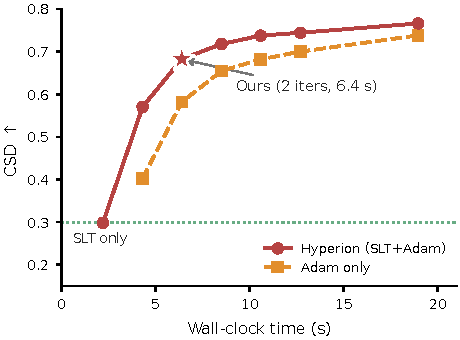
\includegraphics[width=\linewidth]{fig/figure/fig2_pareto.pdf}
  \caption{CSD vs.\ wall-clock trade-off (40-sample subset): Hyperion
    (red) vs.\ Adam-only (orange); $\star$ marks the operating point.}
  \label{fig:iter_tradeoff}
\end{figure}

% ─────────────────────────────────────────────────────────────────────────────
\subsection{Cross-Backbone Generalization}
\label{sec:exp:backbone}

Our Hyperion pipeline targets the MM-DiT family of architectures, which shares the same double-stream self-attention design across models.
To verify generalization, we apply the identical pipeline---same hyperparameters, no retuning---to FLUX.1-dev~\cite{flux2024} (12B parameters), a second MM-DiT model distinct from Klein~9B used in all other experiments.
On the same 40-sample subset (8 styles $\times$ 5 prompts), FLUX.1-dev achieves CSD~$= 0.719$ and CLIP-T~$= 0.291$, versus Klein's CSD~$= 0.681$ and CLIP-T~$= 0.274$.
The higher scores on FLUX.1-dev are consistent with its larger capacity; the key finding is that the pipeline requires no modification.
Full details are in Appendix~\ref{app:flux1dev}.

A T2I benchmark gallery of Hyperion results across diverse styles and content
prompts is provided in the supplement (Fig.~\ref{fig:t2i_benchmark}).

\section{Ablation Study}
\label{sec:ablation}

All ablations use the 40-sample subset (8 styles, \texttt{sty}
00/10/14/20/27/28/33/38, $\times$ 5 prompts) unless otherwise noted.
Quantitative results are shown in Table~\ref{tab:ablation}; a bar-chart
summary is provided in Fig.~\ref{fig:ablation_bar} in the supplementary
material.
The operating point ($\alpha{=}0.10$, $N{=}2$) is itself justified by the
sweeps in Sec.~\ref{sec:ablation:alpha} and~\ref{sec:ablation:adam}; the
component ablation below holds it fixed and removes one component at a time.

% ─────────────────────────────────────────────────────────────────────────────
\subsection{Component Ablation}
\label{sec:ablation:components}

\begin{table}[t]
  \centering
  \caption{%
    Component ablation on the 40-sample subset (8 styles $\times$ 5 prompts, seed~43).
    All numbers from runs at fixed seed~43 on a single H200.
    Wall-clock times are indicative single-run measurements under shared GPU
    load; exclusive-GPU medians for the key configurations appear in
    Fig.~\ref{fig:timing}.
    STM is the Style--Texture Match (Sec.~\ref{sec:exp:texcoh}); it tracks CSD
    across all cells (Pearson $r{=}0.98$), independently confirming each
    component's texture contribution.
    Boldface = best among training-free single-GPU methods.%
  }
  \label{tab:ablation}
  \footnotesize
  \begin{tabular}{lccccc}
    \toprule
    Configuration & CSD & CLIP-T & STM & Fwd. & Time~$\downarrow$ \\
    \midrule
    \rowcolor{tabshade!10}
    \textbf{Ours (Hyperion, $N{=}2$)} & \textbf{0.681} & 0.274 & \textbf{0.775} & 4  & 6.4~s \\
    No SLT (Adam-2)                 & 0.584 & 0.291 & 0.697 & 4  & 6.4~s \\
    No Adam (SLT only)              & 0.298 & 0.309 & 0.624 & 2  & 2.2~s \\
    Softmax attn.\ target           & 0.633 & 0.283 & 0.735 & 4  & 6.4~s \\
    No freq.\ boost                 & 0.678 & 0.271 & 0.773 & 4  & 6.4~s \\
    Adam-8 (upper bound)            & 0.650 & 0.296 & 0.726 & 10 & 19.0~s \\
    \bottomrule
  \end{tabular}
\end{table}

\paragraph{No SLT (Adam-2 only)}
Removing SLT and running 2 Adam iterations alone drops CSD from 0.681 to 0.584
($-$14.2\%).
With only 2 Adam steps and no color pre-alignment, the optimizer spends both
iterations on color convergence rather than texture, reaching neither the color
alignment of SLT nor the texture richness of Adam-8.
This confirms that SLT's contribution is not merely additive but enables Adam
to specialize on texture in fewer iterations.

\paragraph{No Adam (SLT only)}
SLT alone achieves CSD~$= 0.298$, just 44\% of Hyperion's score.
Per the spatial neighbor cosine analysis (Table~\ref{tab:spatial_proof}),
SLT's $\rho = 0.24$ is $2.6\times$ below Adam's $\rho = 0.64$, which
directly explains the absence of brushstroke texture.
SLT is a necessary but insufficient component.

\paragraph{Softmax attention target}
Replacing our doubly-stochastic attention target with standard softmax
($\texttt{scaled\_dot\_product\_attention}$) inside Adam-in-loop
decreases CSD from 0.681 to 0.633 ($-$7.0\%).
Softmax allows column sums to be unconstrained, so a few dominant style tokens
accumulate disproportionate attention weight; the resulting style target is less
informative and the 2 Adam steps cannot recover the full style distribution.
The doubly-stochastic normalization in our attention target provides a richer,
more uniform optimization signal.

\paragraph{No frequency boost}
\label{sec:ablation:freq}
Disabling the high-frequency Sinkhorn boost (\texttt{FREQ\_HI\_BOOST}$=0$)
reduces CSD from 0.681 to 0.678 ($-$0.4\%).
The frequency decomposition and high-frequency boosting recover fine-grained
painterly details (thin brushstrokes, sharp edges) that the standard $\ell_1$
loss with spatial averaging tends to smooth over.
The effect is moderate but consistent across style categories.

\paragraph{Layout residual suppression (LRS)}
LRS is not CSD-scorable in isolation---it suppresses the style image's spatial
\emph{layout}, not its texture statistics---so we evaluate it with a dedicated
layout-leakage metric. Disabling LRS significantly increases layout leakage
(paired $t{=}2.84$, $p<0.01$; Table~\ref{tab:supp_metrics}), and the leaked
composition is directly visible in Fig.~\ref{fig:lrs_demo}.

\paragraph{Seed robustness}
Repeating the 40-sample subset across three seeds $\{43, 44, 45\}$ yields
CSD~$= 0.682 \pm 0.002$ (Hyperion) and $0.650 \pm 0.006$ (Adam-8), and
CLIP-T~$= 0.274 \pm 0.002$ (Hyperion).
The standard deviation over seeds is two orders of magnitude smaller than the
Hyperion-vs-Adam-8 gap; a paired $t$-test over the pooled 120 samples confirms
the gap is highly significant ($t = 8.9$, $p = 7\times10^{-15}$).
The reported point estimates are therefore seed-robust; the full-benchmark
numbers (Table~\ref{tab:main}) use seed~43.

A per-component visual ablation across three content--style examples is provided
in the supplement (Fig.~\ref{fig:ablation_qual}), confirming that each removed
component degrades the output in the way the metrics predict.

% ─────────────────────────────────────────────────────────────────────────────
\subsection{SLT Alpha Sweep}
\label{sec:ablation:alpha}

We sweep the SLT pre-alignment strength $\alpha$
across seven values ($0.0,\,0.02,\,0.05,\,0.10,\,0.20,\,0.30,\,0.50$)
in the SLT-only configuration (Adam disabled), isolating the transport
step's own effect, and record the CSD--CLIP-T trade-off
(Fig.~\ref{fig:alpha_sweep}); the chosen operating point is then validated
inside the full pipeline by the component ablation
(Table~\ref{tab:ablation}).
CSD rises monotonically with $\alpha$, while CLIP-T remains stable up to
$\alpha=0.10$ ($0.309$) and degrades sharply beyond $\alpha=0.20$ ($0.299$,
collapsing to $0.193$ at $\alpha=0.50$); $\alpha=0.10$ balances style
fidelity (CSD $0.298$) against content preservation.

\begin{figure}[t]% 十二修: 从[H]改[t]，让5.2文字回填p14右栏，消除小标题上下被flushbottom撑开的空白
  \centering
  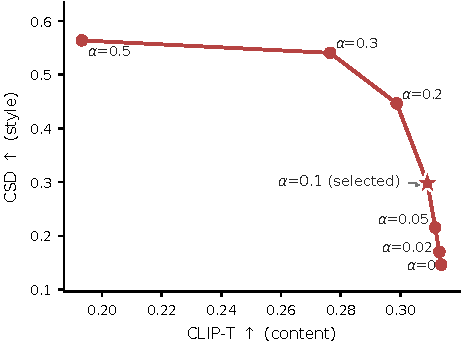
\includegraphics[width=\linewidth]{fig/figure/fig4_slt_sweep.pdf}
  \caption{CSD--CLIP-T trade-off of the SLT strength $\alpha$
    (SLT-only, 40-sample subset); $\star$ marks the selected $\alpha{=}0.10$.}
  \label{fig:alpha_sweep}
\end{figure}
% ─────────────────────────────────────────────────────────────────────────────

$\alpha = 0.10$ is the Pareto-optimal point: lower values ($\alpha \le 0.05$)
leave too much color gap for Adam to resolve in 2 iterations, while higher
values ($\alpha \ge 0.20$) over-transport and suppress the content structure
that Adam's content anchor is designed to preserve.

% ─────────────────────────────────────────────────────────────────────────────
\subsection{Adam Iterations Sweep}
\label{sec:ablation:adam}

Fixing SLT and sweeping Adam iterations $N \in \{1, 2, 3, 4, 5, 6, 7, 8\}$
reveals the cost--quality trade-off of the Adam refinement stage
(Fig.~\ref{fig:adam_sweep}).
Hyperion rises steeply from $N{=}1$ (CSD $0.570$) to $N{=}2$ ($0.682$)
and then saturates, whereas Adam-only requires roughly twice as many
iterations to reach comparable quality; the iteration-free baselines sit at
$0.298$ (SLT-only) and $0.039$ (Inject).

\begin{figure}[H]
  \centering
  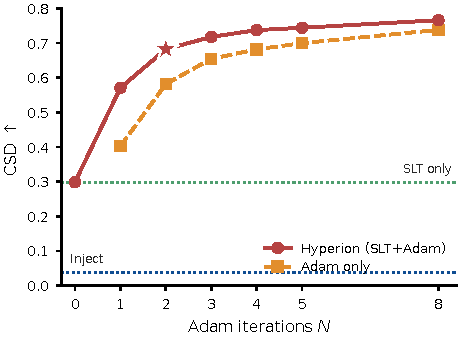
\includegraphics[width=\linewidth]{fig/figure/fig6_iters_sweep.pdf}
  \caption{CSD vs.\ Adam iterations $N$ with (Hyperion) and without
    (Adam-only) SLT pre-alignment; $\bigstar$ marks the selected $N{=}2$.}
  \label{fig:adam_sweep}
\end{figure}
% ─────────────────────────────────────────────────────────────────────────────

After SLT pre-alignment, CSD saturates rapidly: the gain from $N=2$ to $N=3$
is $+0.035$, and beyond $N=3$ each additional iteration yields
$\approx 0.01$ CSD while adding one forward pass per step.
$N=2$ is the default: it captures $\approx 89\%$ of the $N{=}8$ ceiling
($0.682$ vs.\ $0.766$) while keeping total forward passes per step at~4.

\section{Discussion}
\label{sec:discussion}

Having shown that Hyperion leads on both style fidelity and efficiency, we now
examine how to interpret the metrics behind those claims, then discuss failure
modes and the scope of our baseline comparison.

% ─────────────────────────────────────────────────────────────────────────────
\subsection{Metric Considerations}
\label{sec:discussion:metrics}

\paragraph{CSD as primary metric}
The Contrastive Style Descriptor~\cite{somepalli2024measuring} was designed to
measure perceptual style similarity independently of semantic content.
It remains a learned embedding, however, and is not immune to all confounders.
When a method copies the style reference's composition rather than only its
texture (layout leakage), the output and reference share not only style but also
content, inflating CSD.
We mitigate this by applying LRS (Sec.~\ref{sec:method:lrs}) and by
reporting CLIP-T alongside CSD: a method that inflates CSD by composition
copying would show degraded CLIP-T (the content prompt becomes unsatisfied
because a foreign subject now fills the image).
Table~\ref{tab:ablation} confirms that our method maintains CLIP-T while
achieving high CSD, supporting the interpretation that our CSD gains reflect
genuine style transfer rather than layout copying.

\paragraph{CLIP-T and content preservation}
CLIP-T~\cite{radford2021learning} measures semantic similarity of the output to the text prompt.
It is sensitive to dominant compositional changes but may not penalize moderate
texture artifacts.
Outputs with strong style transfer but intact subject placement score similarly
to mild-style outputs; the two are not separable by CLIP-T alone.
For this reason, we present CLIP-T as a \emph{necessary} but not
\emph{sufficient} indicator of content preservation.
Qualitative inspection (Fig.~\ref{fig:qualitative}) provides complementary
evidence.

\paragraph{Forward-pass count as efficiency metric}
Wall-clock timing reported in Table~\ref{tab:ablation} was measured under
concurrent GPU load and should be treated as approximate.
We use \emph{forward passes per denoising step} as the hardware-agnostic
efficiency metric: each Adam iteration (one forward plus one backward pass
per denoising step) adds approximately 2.1~s to total generation time on a
single H200 at our resolution and batch size, and this per-iteration cost is
stable across configurations.
Independent H200 runs (5-trial median, 3 warmup runs) confirm this linear
cost model to within 5\%.

% 十修: C12 — acknowledge the absence of a user study (TPAMI style-transfer
% papers近乎标配; 提前承认比被审稿人点名强).
\paragraph{Absence of a human preference study}
All conclusions in this paper rest on automated metrics (CSD, CLIP-T, CLIP-I,
STM) corroborated by qualitative inspection.
The metric triangulation of Sec.~\ref{sec:exp:texcoh}---which cross-checks the
embedding-space CSD against parameter-free pixel-space texture
statistics---mitigates single-descriptor bias, but a controlled
two-alternative forced-choice user study remains the most direct measure of
\emph{perceived} style fidelity and content preservation.
We have not conducted one, and regard this as a limitation of the present
evaluation.

% ─────────────────────────────────────────────────────────────────────────────
\subsection{Failure Cases and Limitations}
\label{sec:discussion:limitations}

\paragraph{Low-rank style references}
Style \texttt{sty04} (excluded from all evaluations) contains near-uniform
pixel statistics with effective rank below~5.
The SLT transport plan degenerates when $z_s$ spans only a 1--2 dimensional
subspace: the transported content latent collapses to a very small region of
style space, and Adam cannot recover meaningful texture from it.
A pre-screening filter on style diversity (e.g., pixel entropy or latent
effective rank) is recommended for deployment.

\paragraph{Object position drift}
Despite LRS suppression, severe cases of spatial drift remain on some styles
with high-contrast subjects positioned far from the center.
The LRS residual coefficients ($\gamma^{(\ell)}$ from $0.7$ in shallow blocks
to $0.5$ in deep blocks) retain a substantial share of the positional
residual, which is sufficient to cause moderate drift in severe cases.
Reducing $\gamma^{(\ell)}$ further eliminates drift but reduces texture
sharpness; the current setting is a deliberate Pareto compromise.
Both failure modes are most pronounced at $512\times512$; finer sub-token
details and edge cases are expected to improve at higher latent resolution,
which we leave to future work.

\paragraph{Scope of the baseline comparison}
The closest training-free competitors---StyleAligned~\cite{hertz2024style},
V-Shuffle~\cite{vshuffle2025}, and Inversion-Free Dual~RF~\cite{dualrf2025}---were
developed for SDXL and rectified-flow backbones and have no publicly released
implementation for the Klein~9B MM-DiT architecture used here.
Of these, V-Shuffle's value-permutation mechanism ports most directly to the
MM-DiT attention layout: we evaluate a faithful adaptation head-to-head on the
full 234-pair benchmark, where we dominate it on \emph{both} style fidelity and
content alignment (Sec.~\ref{sec:exp}, Fig.~\ref{fig:vshuffle_cmp})---value
permutation transfers incoherent texture on MM-DiT rather than coherent style.
StyleAligned's attention-sharing and Dual~RF's inversion-free coupling are tied
more deeply to architecture-specific layouts (single-stream SDXL self-attention
and rectified-flow sampling, rather than MM-DiT's joint image--text stream and
RoPE positional coupling), so a faithful port is a research effort in its own
right, and an \emph{unvalidated} re-implementation could misrepresent their true
capability.
For those two we therefore do not report numbers we cannot stand behind,
comparing instead against the \textbf{Inject} baseline---a representative of the
attention-manipulation family they refine---and four \emph{trained} style
adapters (StyleShot, USO, CSGO, IP-Adapter) across 21 diverse style families
(Table~\ref{tab:percat}).
Faithful MM-DiT ports of StyleAligned and Dual~RF, validated against their
original results, are the natural next comparison.

\section{Conclusion}
\label{sec:conclusion}

% 九修: conclusion condensed (advisor: slightly longer than the abstract);
% 十修 round 2 audit found it came in ~30 words SHORTER than the abstract
% (218 vs 246) -> mechanism-evidence sentence added to para 2 (~262 words).
We presented Hyperion, a training-free style-transfer pipeline for
MM-DiT built on a systematic analysis of latent-update strategies.
Attention injection fails because a single feedforward substitution cannot
induce spatial coherence; per-token optimal transport (SLT) aligns color
distributions efficiently but produces no texture, since its per-token
independence severs the inter-token coupling that backpropagation exploits
through the attention Jacobian.
The spatial neighbor cosine quantifies this difference: Adam gradients reach
$\rho = 0.64$ whereas SLT updates reach $\rho = 0.24$, explaining the visual
distinction between textured and flat stylization.

Hyperion therefore combines SLT pre-alignment with two Adam refinement
steps, so that Adam is devoted to texture from its first iteration;
frequency-domain Sinkhorn boosting and LRS layout suppression provide
further, independently validated improvements.
Both components rest on mechanism-level evidence: shuffling the spatial
order of the style keys and values leaves the coherence unchanged---so the
coherence originates in the attention Jacobian, not in the layout of the
reference---while the LRS factor attenuates attention-logit variance by
$\gamma^{2}$, making residual layout leakage decay quadratically.
On a benchmark of 39 style references $\times$ 6 content prompts (234 pairs),
Hyperion attains CSD~$=0.640$ and CLIP-T~$=0.296$ with four forward passes
per denoising step---exceeding an 8-iteration Adam-only schedule at
$2.5\times$ lower forward-pass cost---and, despite using no style-specific
training, surpasses four trained style adapters on 19 of 21 diverse style
families; the same pipeline transfers directly to image-to-image
stylization.

Future work includes distilling the style signal into a lightweight side
network to halve the per-step cost, extending the coherence analysis to video
diffusion transformers, and combining the training-free backbone with sparse
fine-tuning on style exemplars.
Code and evaluation scripts will be released upon acceptance to support reproducibility.


\clearpage   % flush all pending floats before references
\balance
\bibliographystyle{IEEEtran}
\bibliography{bib/refs}

% 十三修排版 (2026-07-09): references restored to directly follow the conclusion
% (pre-十二修 order, per advisor). The appendix is kept as one contiguous block at
% the very end so the single-compile PDF (all 60+ cross-refs baked into pixels, no
% xr/??) can be physically split into main.pdf (body+refs) + supplementary.pdf
% (appendix) for the two-file TPAMI submission. supp.tex self-manages
% \clearpage\onecolumn\appendices.
% ============================================================
%  Supplementary Material
% ============================================================
\clearpage
\onecolumn
\appendices

% ─────────────────────────────────────────────────────────────────────────────
\section{Implementation and Reproduction Details}
\label{app:repro}

This appendix collects every setting required to reproduce the main-paper
results: the backbone and generation configuration
(Sec.~\ref{app:repro:backbone}), the complete hyperparameter set of the Hyperion
pipeline and its derived baselines (Sec.~\ref{app:repro:hparams}), the benchmark
composition (Sec.~\ref{app:repro:bench}), the evaluation protocol
(Sec.~\ref{app:repro:eval}), the configuration of every competing method
(Sec.~\ref{app:repro:baselines}), wall-clock timing
(Sec.~\ref{app:repro:timing}), and the software environment
(Sec.~\ref{app:repro:env}). Unless a multi-seed range is stated explicitly, all
reported numbers use the fixed seed~$43$.

\subsection{Backbone and Generation Configuration}
\label{app:repro:backbone}
All main-paper experiments use \textbf{Klein~9B}, an MM-DiT rectified-flow model
with $8$ double-stream and $24$ single-stream blocks ($32$ self-attention layers
in total), driven through the DiffSynth backend in \texttt{bf16} mixed precision
on a single H200 GPU. Images are generated at $512\times512$ with $25$
flow-matching denoising steps, classifier-free guidance scale $3.5$, and fixed
seed~$43$; the packed image latent carries $L=1024$ tokens on a $32\times32$
grid. \emph{No model weights are modified at any point}: the style signal enters
only through frozen forward passes (which read the style keys/values) and the
latent-space SLT and Adam updates. Style injection, SLT pre-alignment, and
Adam-in-loop optimisation are active only for denoising steps with
$t<t_\text{start}$ (on the model's $[0,1000]$ noise schedule), with
$t_\text{start}=850$ for T2I and $870$ for I2I; the earliest high-noise steps run
ordinary denoising so that coarse semantic structure forms before any style is
imposed.
% 十修: availability statement for the backbone checkpoint.
Klein~9B weights are publicly available (FLUX.2~[klein]~9B~\cite{flux2klein2025},
released under the FLUX Non-Commercial License).

\subsection{Hyperion Pipeline Hyperparameters}
\label{app:repro:hparams}
Table~\ref{tab:repro_hparams} lists the full hyperparameter set of the three
per-step stages (LRS $\to$ SLT $\to$ Adam$\times2$), together with the two
derived configurations used as baselines (\textsc{Adam-8} in
Table~\ref{tab:main} and the aggressive \textsc{Adam-only} iteration sweep in
Table~\ref{tab:iter_tradeoff}). Two distinct entropic-regularisation
temperatures appear and must not be conflated: $\tau_{\mathrm{SLT}}=0.02$ governs
the one-shot Sinkhorn \emph{transport plan} of the SLT step (Eq.~\ref{eq:slt}),
whereas $\tau_{\mathrm{attn}}$ governs the entropic-OT \emph{attention} used
inside the frequency-domain style loss (Sec.~\ref{sec:method:freq}), annealed
from $0.15$ to $0.07$ across the active denoising window.

\begin{table}[t]
  \centering
  \caption{Complete hyperparameters of the Hyperion pipeline
           (LRS\,$\to$\,SLT\,$\to$\,Adam$\times2$) and the two derived baselines.
           $\tau_{\mathrm{SLT}}$ (transport plan) and $\tau_{\mathrm{attn}}$
           (style-loss OT attention) are distinct quantities.}
  \label{tab:repro_hparams}
  \footnotesize
  \begin{tabular}{@{}ll@{}}
    \toprule
    Component / parameter & Value \\
    \midrule
    \multicolumn{2}{@{}l}{\textit{SLT pre-alignment (Eq.~\ref{eq:slt})}}\\
    \quad mixing strength $\alpha$ & $0.10$ \\
    \quad Sinkhorn temperature $\tau_{\mathrm{SLT}}$ & $0.02$ \\
    \quad Sinkhorn iterations & $10$ \\
    \quad ground cost & cosine sim.\ of high-freq.\ residuals $z-\bar z$ \\
    \quad application & OT-AdaIN, per-token $\mu^\ast,\sigma^\ast$ \\
    \midrule
    \multicolumn{2}{@{}l}{\textit{Adam-in-loop (Hyperion)}}\\
    \quad iterations $N$ & $2$ \\
    \quad learning rate & $0.03$ \\
    \quad style weight $w_s$ & $2.0$ \\
    \quad content-anchor weight $w_c$ & $1.5$ \\
    \quad loss & $\ell_1$ on style $+$ content (Eq.~\ref{eq:adam_loss}) \\
    \quad optimiser & Adam, $(\beta_1,\beta_2){=}(0.9,0.999)$, wd $0$ \\
    \midrule
    \multicolumn{2}{@{}l}{\textit{Frequency-domain style loss (Sec.~\ref{sec:method:freq})}}\\
    \quad high-freq.\ boost $\gamma_{\mathrm{hi}}$ & $2.0$ \\
    \quad OT-attention layers & deepest $50\%$ of self-attn.\ layers \\
    \quad OT-attention temp.\ $\tau_{\mathrm{attn}}$ & $0.15\!\to\!0.07$ (annealed) \\
    \quad OT-attention Sinkhorn iters & $6$ \\
    \midrule
    \multicolumn{2}{@{}l}{\textit{LRS (Eq.~\ref{eq:lrs})}}\\
    \quad residual coeff.\ $\gamma^{(\ell)}$ & $0.7$ (shallow) $\to 0.5$ (deep), linear \\
    \quad applied to & style $K$ and $V$ \\
    \midrule
    % 十修: removed the old "content-init AdaIN alpha_ada" row (mechanism
    % direction was reversed relative to the code; there is no content-target
    % AdaIN). Its alpha=0.3 value is the I2I-side entry already carried by the
    % "per-step AdaIN warm-start alpha_w" row below (Auxiliary color
    % operations), so it is not repeated here. Added the true I2I
    % content-conditioning mechanism (in-context concatenation) instead.
    \multicolumn{2}{@{}l}{\textit{I2I only (Sec.~\ref{sec:method:i2i})}}\\
    \quad content conditioning & in-context token concatenation
      (structural, every step, no hyperparameter) \\
    \quad injection start $t_\text{start}$ & $870$ (T2I: $850$) \\
    \midrule
    % 十修: auxiliary color operations added to the hyperparameter table
    % (previously present in code only; see Algorithm~\ref{alg:pipeline} and
    % Sec.~\ref{sec:method:hybrid} for the disclosure and ablation).
    \multicolumn{2}{@{}l}{\textit{Auxiliary color operations}}\\
    \quad per-step AdaIN warm-start $\alpha_w$ & $0.5$ (T2I), $0.3$ (I2I) \\
    \quad warm-start timing / target & every active step, after LRS, before SLT; toward noised style latent \\
    \quad terminal color correction & 1-D AdaIN, once after the denoising loop; toward clean style latent \\
    \quad terminal correction gate & on by default; off only for text-only / raw-injection baselines \\
    \midrule
    \multicolumn{2}{@{}l}{\textit{Derived baselines (no SLT)}}\\
    \quad Adam-8 (Table~\ref{tab:main}) & $N{=}8$, lr $0.01$, $w_c{=}0.2$, $w_s{=}2.0$ \\
    \quad Adam-only sweep (Table~\ref{tab:iter_tradeoff}) & lr $0.03$, $w_c{=}1.5$, $w_s{=}2.0$ \\
    \bottomrule
  \end{tabular}
\end{table}

\subsection{Benchmark Composition}
\label{app:repro:bench}
\paragraph{Styles} The style bank holds $40$ reference images
(\texttt{sty00}--\texttt{sty39}); \texttt{sty04} is excluded from all evaluation
for degenerate (near-uniform, effective-rank ${<}5$) pixel statistics, leaving
$39$ styles for the full T2I benchmark.

\begin{figure*}[t]
  \centering
  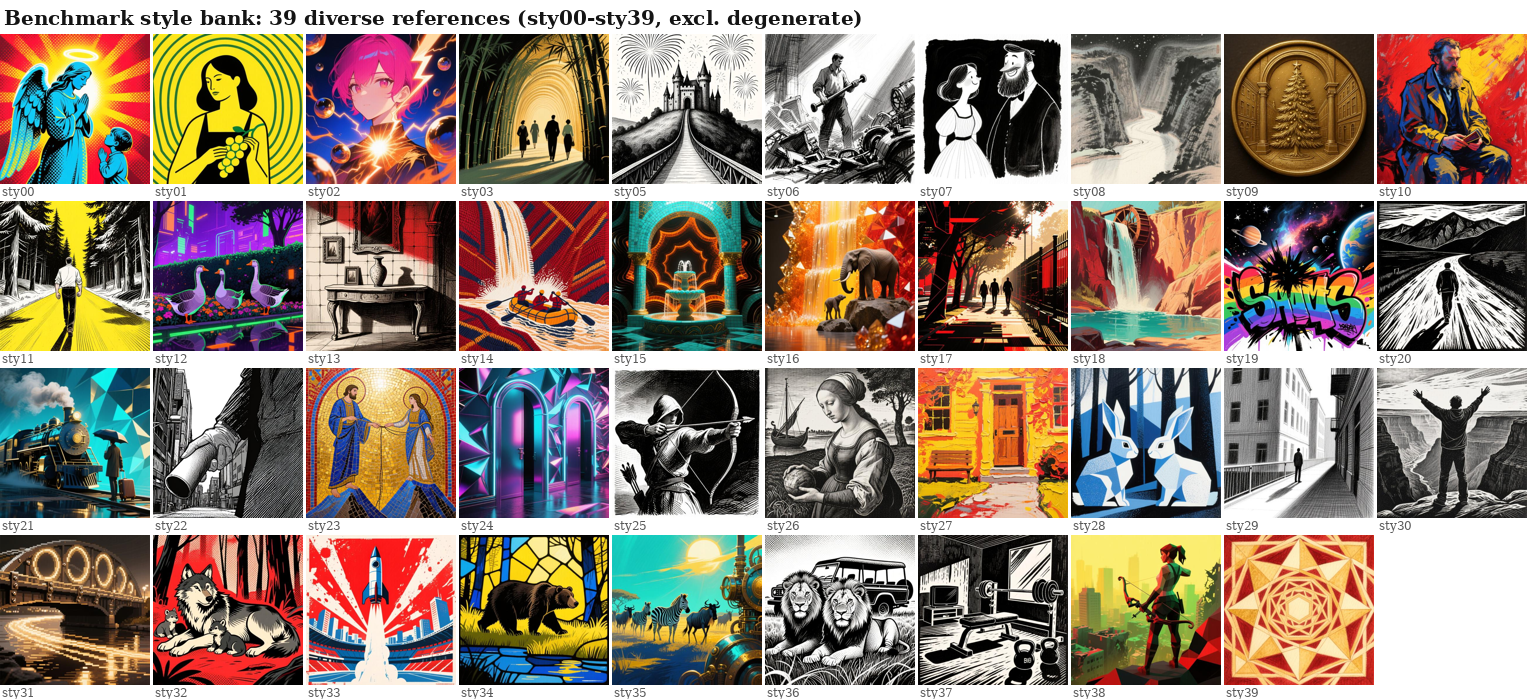
\includegraphics[width=\linewidth]{figures_hires/fig_benchmark_atlas.png}
  \caption{The constructed benchmark style bank: 39 mutually distinct style
    references (\texttt{sty00}--\texttt{sty39}, excluding the degenerate
    \texttt{sty04}) spanning traditional media (oil, watercolor, ink, bronze
    relief, ukiyo-e), graphic and illustrative styles (posters, screenprint,
    art-deco, constructivist, comic), digital/pixel art, and photographic
    textures. Each reference is paired with all six content prompts
    (Table~\ref{tab:prompts}) to form the $234$-pair T2I benchmark.}
  \label{fig:benchmark_atlas}
\end{figure*}

\paragraph{T2I content} Six fixed prompts (Table~\ref{tab:prompts}) give
$39\times6=234$ evaluation pairs. The ablation / sweep / robustness subset uses
$8$ representative styles (\texttt{sty}\,00/10/14/20/27/28/33/38) $\times$ $5$
prompts (``A panda eat bamboo'', ``A castle on a cliff by the sea'', ``A cat
sitting on a windowsill'', ``A field of sunflowers at sunset'', ``A portrait of
an old fisherman''), i.e.\ $40$ pairs.
\paragraph{I2I content} Nineteen content photographs
(\texttt{cnt00}--\texttt{cnt18}) give a $39\times19=741$-pair full I2I benchmark;
the I2I subset is the same $8$ styles $\times$ $5$ content images
(\texttt{cnt}\,00/04/08/12/17) $=40$ pairs.
\paragraph{Trained-baseline comparison} The $21$-family comparison
(Table~\ref{tab:percat},
Figs.~\ref{fig:trained_baselines}--\ref{fig:trained_baselines_c}) uses the single
prompt ``A panda eat bamboo''.
\paragraph{Seeds} All quantitative tables use seed~$43$; the multi-seed
robustness analysis uses seeds $\{43,44,45\}$; the qualitative tiles in
Figs.~\ref{fig:diverse_main} and
\ref{fig:trained_baselines}--\ref{fig:trained_baselines_c} display the best of six
seeds $\{43\text{--}48\}$ selected jointly on CSD and CLIP-T (never used for any
reported number).

\subsection{Evaluation Protocol}
\label{app:repro:eval}
All three primary metrics are computed identically across methods on the final
decoded RGB outputs. \textbf{CSD} is the Contrastive Style Descriptor
similarity~\cite{somepalli2024measuring}: output and style reference are encoded
with the released CSD model (ViT-L/14 backbone, authors' checkpoint) and we take
the cosine similarity of the $\ell_2$-normalised style embeddings.
\textbf{CLIP-T} and \textbf{CLIP-I} use OpenAI CLIP ViT-B/32 (via
\texttt{open\_clip}): CLIP-T is the cosine similarity between the output-image
embedding and the prompt-text embedding; CLIP-I (I2I only) is the cosine
similarity between the output and content-image embeddings. Every image is
preprocessed by bicubic resize to $224$, a $224$ centre-crop, and CLIP
normalisation, so all metrics are \emph{resolution-agnostic}: baselines that
generate at $1024^2$ (Sec.~\ref{app:repro:baselines}) are compared at their
native resolution with no penalty. The supplementary perceptual metrics
(DINOv2-style, VGG-19 Gram distance, and layout leakage in
Sec.~\ref{app:supp_metrics}; LPIPS, ArtFID, and texture coherence in
Sec.~\ref{app:newmetrics}) use the same loading pipeline.

\subsection{Baseline Configurations}
\label{app:repro:baselines}
Table~\ref{tab:repro_baselines} gives the exact configuration of every competing
method. The two training-free references are implemented directly in our pipeline
(\textbf{Inject}: style $K/V$ blended into the image-token attention with
$\beta=0.5$, two forward passes and no backward pass; \textbf{V-Shuffle}:
identical, but the style \emph{value} tokens are spatially permuted before
attention, Sec.~\ref{sec:exp:main}). The four trained adapters are run from their
official releases at their recommended settings; because every metric is
computed at $224$ (above), running the trained adapters at their native
$1024^2$ is the configuration most favourable to them.

\begin{table}[t]
  \centering
  \caption{Configuration of every competing method. Training-free references
           (Inject, V-Shuffle) are implemented in our own pipeline; the four
           trained adapters are run from their official releases.}
  \label{tab:repro_baselines}
  \footnotesize
  \setlength{\tabcolsep}{4pt}
  \begin{tabular}{@{}llcp{7.6cm}@{}}
    \toprule
    Method & Base model & Res. & Key settings \\
    \midrule
    Inject     & Klein~9B   & $512$  & training-free; style $K/V$ inject $\beta{=}0.5$; 2 fwd, no backward \\
    V-Shuffle  & Klein~9B   & $512$  & training-free; as Inject $+$ style-$V$ spatial permutation; faithful full injection $\beta{=}1.0$; 2 fwd, no backward \\
    StyleShot  & SD-1.5     & $512$  & trained; 50 steps, guidance $7.5$, seed $42$ \\
    USO        & FLUX.1-dev & $1024$ & trained; LoRA rank $128$ $+$ projector, 25 steps, guidance $4.0$, seed $3407$ \\
    CSGO       & SDXL       & $1024$ & trained; 4 content / 32 style tokens, 50 steps, guidance $7$, content-scale $0.01$, seed $42$ \\
    IP-Adapter & FLUX.1-dev & $1024$ & trained; XLabs flux-ip-adapter, ip-scale $1.0$, 25 steps, guidance $4.0$, seed $3407$ \\
    \bottomrule
  \end{tabular}
\end{table}

\subsection{Wall-Clock Timing}
\label{app:repro:timing}
Fig.~\ref{fig:timing} reports per-method wall-clock time (median of five runs on
a single H200). SLT alone adds ${<}0.01$~s over the no-style baseline
($2.2$~s); the Hyperion pipeline at $N{=}2$ runs in $6.4$~s---a $3.0\times$ speedup
over Adam$\times8$ ($19.0$~s) at \emph{higher} style fidelity. Because absolute
times depend on concurrent GPU load, the main paper uses forward passes per
denoising step (Table~\ref{tab:main}) as the hardware-agnostic cost metric; the
timing below is the supporting wall-clock view.

\begin{figure}[t]
  \centering
  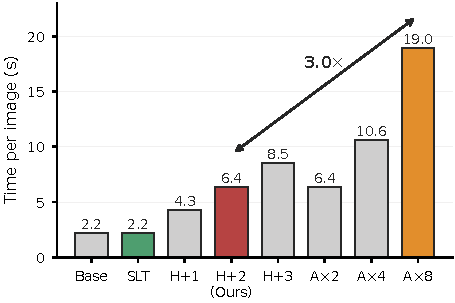
\includegraphics[width=0.48\linewidth]{fig/figure/fig5_timing.pdf}
  \caption{%
    Wall-clock time on a single H200 GPU (median of 5 runs).
    SLT adds ${<}0.01$~s over the no-style baseline; Hyperion (SLT\,$+$\,Adam$\times2$)
    runs in $6.4$~s---$3.0\times$ faster than Adam$\times8$ ($19.0$~s) with
    \emph{higher} style fidelity.%
  }
  \label{fig:timing}
\end{figure}

\subsection{Software Environment}
\label{app:repro:env}
Generation uses the DiffSynth MM-DiT backend with \texttt{diffusers}~0.37.0.dev0
and PyTorch in \texttt{bf16}; metric evaluation uses \texttt{open\_clip}
(CLIP ViT-B/32), the released CSD model (ViT-L/14), DINOv2~\cite{oquab2024dinov2},
torchvision VGG-19, and LPIPS (AlexNet). All randomness is seeded; reported
numbers use seed~$43$.

% ─────────────────────────────────────────────────────────────────────────────
\section{Formal Analysis of the Backpropagation Gap}
\label{app:jacobian}

\subsection{Setup}

We analyze single-head self-attention; the multi-head case follows by applying
the same argument to each head and summing.
Let $z \in \mathbb{R}^{L \times D}$ denote the content latent and
$W_Q, W_K, W_V \in \mathbb{R}^{D \times d}$ the projection matrices for one
head.
Define content features $Q_c = zW_Q$, $K_c = zW_K$, $V_c = zW_V$,
and let $K_s, V_s \in \mathbb{R}^{L \times d}$ denote the fixed style features
(not functions of $z$).
Let $A^c = \mathrm{softmax}(Q_c K_c^\top / \sqrt{d})$ and
$A^s = \mathrm{softmax}(Q_c K_s^\top / \sqrt{d})$ be the content- and
style-attention matrices.
Define the attention outputs $O_c = A^c V_c$ and $O_s = A^s V_s$, the residual
$R = O_s - O_c \in \mathbb{R}^{L \times d}$, and the (squared Frobenius)
style loss
\begin{equation}
  \mathcal{L}(z) = \|O_s(z) - O_c(z)\|_F^2 = \|R\|_F^2.
  \label{eq:supp_loss}
\end{equation}
We write $g_i = \nabla_{z_i}\mathcal{L} \in \mathbb{R}^D$ for the gradient at
token position $i$.

\subsection{Gradient Decomposition}

By the chain rule,
\begin{equation}
  g_i
  = \sum_{j=1}^{L} \left(
      \frac{\partial O_{s,j}}{\partial z_i}
    - \frac{\partial O_{c,j}}{\partial z_i}
    \right)^\top\! 2R_j.
  \label{eq:supp_chain}
\end{equation}

\paragraph{Style branch}
$O_{s,j} = \sum_k A_{jk}^s V_{s,k}$ with $K_s, V_s$ fixed.
Since $A_{jk}^s$ depends on $Q_j = z_j W_Q$ only, we have
$\partial O_{s,j}/\partial z_i \neq 0$ only when $i = j$.
The style branch therefore contributes a \emph{query-path} term $g_i^Q$ that
is local to token $i$.

\paragraph{Content branch}
$O_{c,j} = \sum_k A_{jk}^c z_k W_V$ with both $A^c$ and $V_c$ depending on $z$.
Differentiating with respect to $z_i$ yields two contributions:
\begin{align}
  \frac{\partial O_{c,j}}{\partial z_i}
  &= \underbrace{A_{ji}^c\, W_V^\top}_{\text{value path}}
   + \underbrace{\sum_k (z_k W_V)^\top \frac{\partial A_{jk}^c}{\partial z_i}}_{\text{QK path}}.
  \label{eq:supp_decomp}
\end{align}

The \emph{value path} $A_{ji}^c W_V^\top$ is non-zero for all pairs $(i,j)$:
token $i$'s value propagates to the output of every token $j$ that attends to
key $i$, weighted by $A_{ji}^c$.
Summing over all $j$ in~\eqref{eq:supp_chain}, the value-path gradient at
token $i$ is
\begin{equation}
  g_i^{\mathrm{val}}
  = -2\,W_V \underbrace{\sum_{j=1}^{L} A_{ji}^c\, R_j}_{\displaystyle\mathbf{r}_i},
  \label{eq:supp_gval}
\end{equation}
where $\mathbf{r}_i \in \mathbb{R}^d$ is a weighted sum of the residual vectors
across \emph{all} positions, with weights given by the $i$-th column of the
attention matrix $A^c$.

The \emph{QK path} contributes an additional term $g_i^K$ through the
dependence of $A^c$ on the query and key projections.
Unlike the value path, this term is not strictly local: $A_{jk}^c$ depends
on $K_i$ for \emph{every} $i$ through the softmax normalizer, so $g_i^K$
couples tokens in principle.
Empirically, however, it is subdominant: on our 40-sample ablation set the
query-side term is small relative to the value-path term, and the stop-grad
ablation (Fig.~\ref{fig:jacobian_ablation}) shows that removing the query-side
gradient path leaves spatial coherence unchanged.
The value-path term therefore carries the spatial coherence signal.
The full gradient decomposes as
\begin{equation}
  g_i = g_i^Q + g_i^{\mathrm{val}} + g_i^K.
  \label{eq:supp_full}
\end{equation}

\subsection{Spatial Coherence Theorem}

\begin{theorem}[Spatial gradient coherence under $\epsilon$-smooth keys]
\label{thm:spatial}
Assume that for spatially adjacent tokens $i$ and $i{+}1$ on the latent grid,
the content keys satisfy
\begin{equation}
  \|K_{c,i} - K_{c,i+1}\|_2 \leq \epsilon\sqrt{d}
  \label{eq:supp_smooth}
\end{equation}
for some $\epsilon \geq 0$.
Then, provided $q_{\max}\epsilon \leq 1$ with
$q_{\max} \coloneqq \max_j \|Q_j\|_2$, the value-path gradients defined
in~\eqref{eq:supp_gval} satisfy
\begin{equation}
  \cos\!\left(g_i^{\mathrm{val}},\, g_{i+1}^{\mathrm{val}}\right)
  \;\geq\; 1 - \frac{C\,\epsilon^2\,\|R\|_F^2}{\|g^{\mathrm{val}}\|_{\min}^2},
  \qquad
  C = 2e^2\,\|W_V\|_2^2\, q_{\max}^2\, L,
  \label{eq:supp_bound}
\end{equation}
where $\|g^{\mathrm{val}}\|_{\min} = \min(\|g_i^{\mathrm{val}}\|, \|g_{i+1}^{\mathrm{val}}\|)$.
\end{theorem}

\begin{IEEEproof}
We bound $\|\mathbf{r}_i - \mathbf{r}_{i+1}\|$ and apply Cauchy-Schwarz.

\emph{Step 1: Key smoothness implies attention smoothness.}
Fix a query row $j$ and write $s_a = Q_j K_a^\top/\sqrt{d}$ for the attention
logit of key $K_a$.
For two keys $K_a, K_b$,
\begin{equation}
  |s_a - s_b|
  = \bigl|Q_j (K_a - K_b)^\top\bigr|/\sqrt{d}
  \leq \frac{\|Q_j\|_2\,\|K_a - K_b\|_2}{\sqrt{d}}
  \leq q_{\max}\,\epsilon,
  \label{eq:supp_logit_diff}
\end{equation}
using assumption~\eqref{eq:supp_smooth} and
$q_{\max} = \max_j\|Q_j\|_2 \leq \|W_Q\|_2 \max_j \|z_j\|_2$.
Because $A^c_{ja}$ and $A^c_{jb}$ are two components of the \emph{same}
softmax vector (identical normalizer), their ratio is exactly
$e^{s_a - s_b}$, hence
\begin{equation}
  \bigl|A_{ja}^c - A_{jb}^c\bigr|
  = A_{jb}^c\,\bigl|e^{s_a - s_b} - 1\bigr|
  \leq e^{|s_a - s_b|} - 1
  \leq e\, q_{\max}\,\epsilon
  \;\eqqcolon\; \mu,
  \label{eq:supp_attn_diff}
\end{equation}
where the last step uses $A_{jb}^c \leq 1$ and
$e^x - 1 \leq e\,x$ for $x \in [0,1]$, valid by the assumption
$q_{\max}\epsilon \leq 1$.
This bound is self-contained and requires no external Lipschitz lemma.

\emph{Step 2: Bound on $\|\mathbf{r}_i - \mathbf{r}_{i+1}\|$.}
From~\eqref{eq:supp_gval},
\begin{align}
  \|\mathbf{r}_i - \mathbf{r}_{i+1}\|_2
  &= \Bigl\|\sum_j (A_{ji}^c - A_{j,i+1}^c) R_j\Bigr\|_2 \notag\\
  &\leq \sum_j |A_{ji}^c - A_{j,i+1}^c|\,\|R_j\|_2
   \leq \mu \sum_j \|R_j\|_2
   \leq \mu\sqrt{L}\,\|R\|_F,
  \label{eq:supp_r_diff}
\end{align}
where the last step uses Cauchy-Schwarz ($\sum_j\|R_j\|_2 \leq \sqrt{L}\,\|R\|_F$).

\emph{Step 3: Cosine lower bound.}
Since $g_i^{\mathrm{val}} = -2W_V\mathbf{r}_i$ and
$g_{i+1}^{\mathrm{val}} = -2W_V\mathbf{r}_{i+1}$,
\begin{align}
  1 - \cos(g_i^{\mathrm{val}}, g_{i+1}^{\mathrm{val}})
  &\leq \frac{\|g_i^{\mathrm{val}} - g_{i+1}^{\mathrm{val}}\|^2}{2\,\|g^{\mathrm{val}}\|_{\min}^2}
   = \frac{4\|W_V(\mathbf{r}_i-\mathbf{r}_{i+1})\|^2}{2\,\|g^{\mathrm{val}}\|_{\min}^2} \notag\\
  &\leq \frac{2\|W_V\|_2^2\,\mu^2 L\,\|R\|_F^2}{\|g^{\mathrm{val}}\|_{\min}^2}.
  \label{eq:supp_cos_step}
\end{align}
Substituting $\mu = e\,q_{\max}\epsilon$
from~\eqref{eq:supp_attn_diff} gives~\eqref{eq:supp_bound} with the explicit
constant $C = 2e^2\|W_V\|_2^2\,q_{\max}^2\,L$.
We deliberately keep $C$ explicit: with $L = 1024$ tokens at $32\times32$
resolution, the bound is informative precisely when
$\epsilon \ll \|g^{\mathrm{val}}\|_{\min} /
(\sqrt{L}\,e\,q_{\max}\|W_V\|_2\|R\|_F)$, i.e.\ in the spatially smooth key
regime; the constant is not absorbable without losing this quantitative
content.
\end{IEEEproof}

\begin{remark}[$\ell_1$ style loss]
The main text optimizes an $\ell_1$ style loss (Eq.~\ref{eq:adam_loss}),
whereas the analysis above uses the squared Frobenius loss
\eqref{eq:supp_loss} for differentiability.
Under the $\ell_1$ loss, the residual $R_j$ in~\eqref{eq:supp_gval} is
replaced by its elementwise subgradient $\mathrm{sign}(R_j)$; the derivation
is otherwise unchanged, and the bound retains the same form with
$\|R\|_F^2$ replaced by $\|\mathrm{sign}(R)\|_F^2 = Ld$.
\end{remark}

\begin{remark}[Validity in MM-DiT]
In Klein~9B, keys are formed as $K_{c,i} = z_i W_K \mathbf{R}(\mathbf{p}_i)$
where $\mathbf{R}(\mathbf{p}_i)$ is the RoPE rotation matrix at grid
position $\mathbf{p}_i$.
For adjacent tokens on the $32\times32$ grid, the rotation difference satisfies
$\|\mathbf{R}(\mathbf{p}_i) - \mathbf{R}(\mathbf{p}_{i+1})\|_F = O(\pi/N_\text{grid}) \approx 0.098$,
which bounds the \emph{rotation-induced} part of the key difference.
The full key difference additionally depends on the latent difference
$\|z_i - z_{i+1}\|_2$, so the RoPE bound alone does not determine $\epsilon$.
We therefore treat $\epsilon$-smoothness~\eqref{eq:supp_smooth} as an
assumption, structurally motivated by the RoPE bound. Direct measurement of
$\|K_{c,i} - K_{c,i+1}\|_2/\sqrt{d}$ on real denoising trajectories in fact
gives a \emph{large} $\epsilon \approx 0.92$ (mean over 40 pairs), so the
coherence bound below is best read as an idealized motivation; the
spatial-coherence conclusion itself is corroborated empirically by the measured
adjacent-token gradient cosine $\rho \approx 0.64$
(Fig.~\ref{fig:spatial_proof}).
\end{remark}

\subsection{Why SLT Lacks Spatial Coupling}

The SLT update at token $i$ is
\begin{equation}
  \Delta_i = \alpha\,(T_{i:}\,z_s - z_{t,i}),
  \label{eq:supp_slt}
\end{equation}
where $T_{i:}$ is the $i$-th row of the doubly-stochastic Sinkhorn plan.
The plan is computed from pairwise cosine similarities
$S_{ij} = \cos(z_{t,i}, z_{s,j})$ and is then applied as a \emph{fixed}
(gradient-detached) transport matrix, exactly as in our implementation.
With $T$ held fixed,
$\partial\Delta_i/\partial z_{t,j} = -\alpha\,\delta_{ij}\,I$: the
cross-token derivative vanishes identically.
The dependence of $T$ itself on the full set of content tokens (through the
Sinkhorn normalization) enters only the \emph{construction} of the plan; it
does not couple the applied updates.
Therefore $\Delta_i$ and $\Delta_{i+1}$ are computed independently, and their
cosine similarity is determined only by coincidental similarity between the
transport targets $T_{i:}z_s$ and $T_{(i+1):}z_s$.
This accounts for the empirically low $\rho_\text{SLT} = 0.24$: the small
positive value reflects mild spatial smoothness of the style latent $z_s$
itself, not any structural coupling mechanism.

Both Normal and Stop-grad-$Q$ achieve $\rho \approx 0.65$--$0.71$ while Random
yields $\rho \approx 0.00$, confirming the value-path interpretation
(Fig.~\ref{fig:jacobian_ablation}).
Note that Stop-grad-$Q$ converges at nearly the same rate in loss
(Fig.~\ref{fig:jacobian_ablation}a), confirming that detaching the query-path
gradient does not materially affect convergence speed, and---more
importantly---has no effect on $\rho$.

\begin{figure}[t]
  \centering
  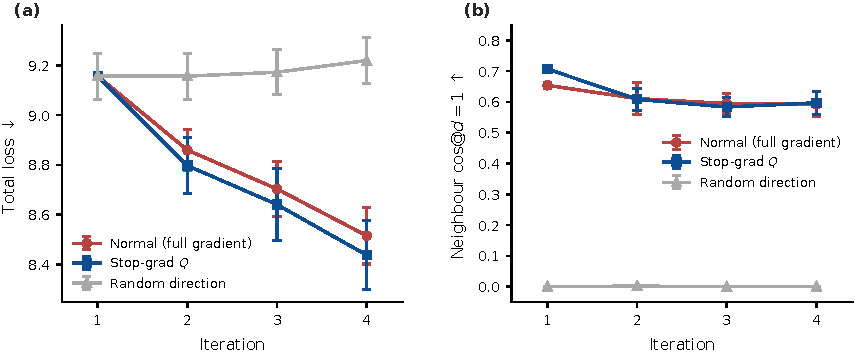
\includegraphics[width=0.95\linewidth]{fig/figure/fig13_jacobian_ablation.pdf}
  \caption{%
    \textbf{(a)} Total style loss under three gradient conditions across 4
    Adam iterations.
    Normal and Stop-grad-$Q$ converge at nearly the same rate; Random direction
    stagnates entirely.
    \textbf{(b)} Spatial neighbor cosine $\rho$ under the same conditions.
    Normal and Stop-grad-$Q$ both maintain $\rho \approx 0.65$--$0.71$;
    Random direction remains at $\rho \approx 0.00$.
    The query-side Jacobian path is not the source of spatial coherence;
    the value-path coupling $g_i^{\mathrm{val}}$ (Eq.~\ref{eq:gval}) is the
    dominant mechanism.%
  }
  \label{fig:jacobian_ablation}
\end{figure}

\begin{figure}[t]
  \centering
  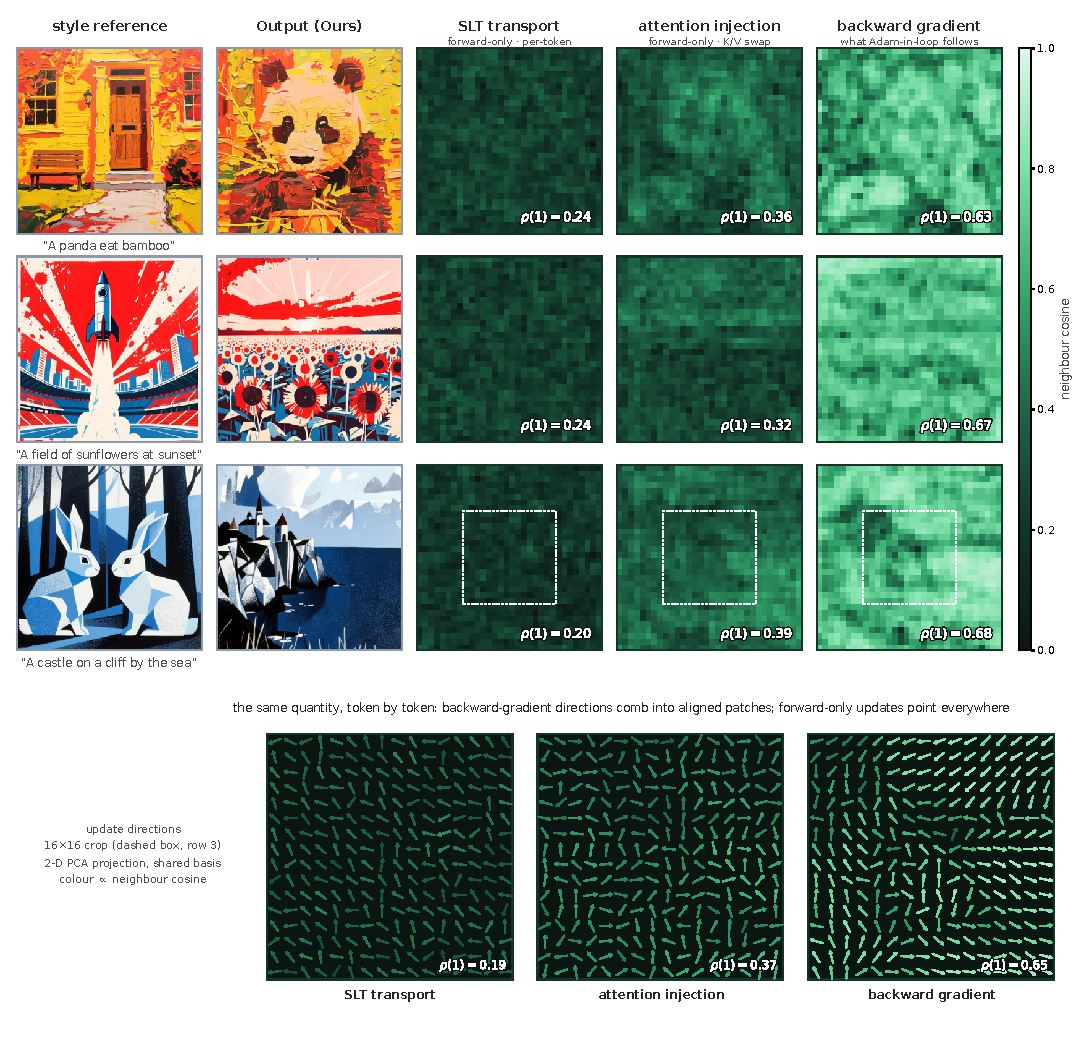
\includegraphics[width=\linewidth]{fig/figure/fig8_coherence_v3.pdf}
  \caption{Neighbour-coherence maps of per-token update directions;
  each map's mean is the $\rho(1)$ of Eq.~\ref{eq:rho}. Forward-only updates
  (SLT $0.24$, attention injection $0.35$) are spatially incoherent, whereas
  backward gradients ($0.64$) organise into content-aligned patches.
  Bottom: the direction fields themselves on a $16{\times}16$ crop---combed
  versus scrambled.}
  \label{fig:pca_maps}
\end{figure}

% ─────────────────────────────────────────────────────────────────────────────
\section{Convergence Analysis: Why Hyperion Outperforms Pure Adam}
\label{app:hybrid}

% 十修: A4 按作者意见主文命题已恢复定量形式（见 sec:method:hybrid,
% prop:hybrid 及其后的 idealized-1.9x / 实测常数 caveat）；本处衔接句相应更新，
% 不再称主文命题为 "now-qualitative"。
This appendix gives the complete derivation and proof of the
pre-alignment efficiency result stated as Proposition~\ref{prop:hybrid} in
the main text (Sec.~\ref{sec:method:hybrid}), together with the assumptions
(A1--A3) under which the quantitative bound holds and a comparison of the
idealized bound against the directly profiled constants
(Remark~\ref{rem:measured_constants}).

\subsection{Loss Decomposition}

We decompose the style loss via the frequency separation introduced in
Sec.~\ref{sec:method:freq}:
\begin{equation}
  \mathcal{L}(z) = \mathcal{L}_c(z) + \mathcal{L}_t(z),
  \label{eq:supp_decomp_loss}
\end{equation}
where $\mathcal{L}_c$ captures color-distribution mismatch (low spatial
frequencies) and $\mathcal{L}_t$ captures texture/high-frequency alignment.
Let $g_c = \nabla_z\mathcal{L}_c$ and $g_t = \nabla_z\mathcal{L}_t$
so that $g = g_c + g_t$.

\paragraph{Empirical orthogonality and frequency profile}
Fig.~\ref{fig:freq_decomp} profiles the SLT and Adam-backward update directions
on the 40-sample subset. Their cosine similarity stays near zero across
iterations (mean $\approx -0.14$; panel~a), empirically supporting the
near-orthogonality $\langle g_c, g_t\rangle \approx 0$ assumed below. Panel~(b)
shows the two mechanisms are \emph{not} cleanly frequency-separated---the SLT
displacement carries $27\%$ low- / $73\%$ high-frequency energy while the Adam
update is closer to balanced ($\approx 49\%/51\%$)---so their complementarity is
one of orthogonal \emph{directions} rather than disjoint frequency bands.

\begin{figure}[t]
  \centering
  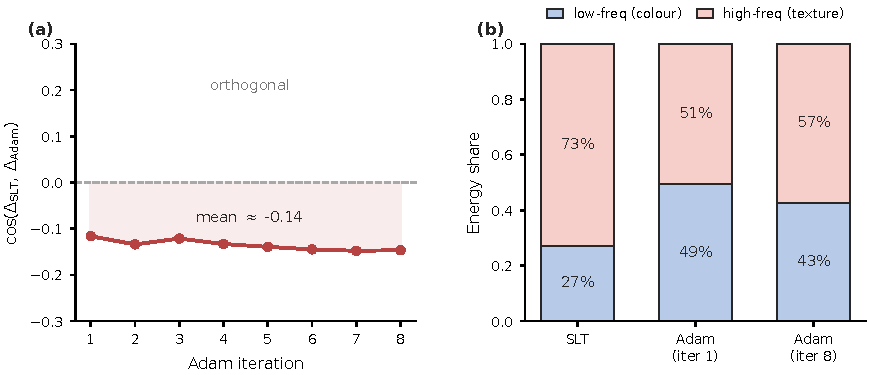
\includegraphics[width=0.97\linewidth]{fig/figure/fig17_freq_decomp.pdf}
  \caption{%
    Frequency / direction decomposition of the SLT and Adam-backward updates
    (40-sample subset).
    \emph{(a)} Per-iteration cosine between the two update directions stays near
    $-0.14$, confirming they are near-orthogonal.
    \emph{(b)} Low- vs high-frequency energy share: SLT is high-frequency-heavy
    ($27/73$) and Adam is near-balanced, so the mechanisms are complementary by
    direction, not by frequency band.%
  }
  \label{fig:freq_decomp}
\end{figure}

\subsection{Assumptions}

\begin{assumption}[Initial color dominance]\label{ass:A1}
At the denoising starting point $z^{(0)}$,
\begin{equation}
  \|g_c(z^{(0)})\|^2 \geq \kappa^2\,\|g(z^{(0)})\|^2
  \label{eq:supp_A1}
\end{equation}
for some $\kappa \in (0,1)$.
We carry $\kappa \approx 0.85$ as an \emph{idealized} working constant for the
bound below. Direct profiling of the first three Adam iterations on the
40-sample subset in fact gives a smaller $\kappa \approx 0.67$ (std $0.23$);
the gap is discussed in Remark~\ref{rem:measured_constants}.
\end{assumption}

\begin{assumption}[SLT color resolution]\label{ass:A2}
After SLT pre-alignment,
\begin{equation}
  \|g_c(z^\mathrm{SLT})\|^2 \leq \epsilon^2\,\|g(z^\mathrm{SLT})\|^2
  \label{eq:supp_A2}
\end{equation}
for some $\epsilon \ll 1$.
Empirically the low-frequency (color) component of the loss drops
substantially after the SLT step, motivating the assumption; we do not rely on
a precise drop fraction.
\end{assumption}

\begin{assumption}[Lipschitz texture gradient]\label{ass:A3}
The texture gradient $g_t$ is $\beta$-Lipschitz in $z$ (a standard smoothness
condition for twice-differentiable losses~\cite{kingma2015adam}), and the SLT
displacement satisfies
$\|z^\mathrm{SLT} - z^{(0)}\| = \alpha\,\|\hat{z}_t - z_t\|
\leq \alpha\,(\|z_s\| + \|z_t\|)$,
with $\alpha = 0.10$ the SLT mixing strength from~\eqref{eq:slt}
(the OT-AdaIN output $\hat{z}_t$ is bounded by the style token statistics,
so the displacement norm is $O(\|z_s\|)$).
Together these give
\begin{equation}
  \|g_t(z^\mathrm{SLT}) - g_t(z^{(0)})\|
  \leq \beta\alpha\,\bigl(\|z_s\| + \|z^{(0)}\|\bigr)
  \eqqcolon \delta\,\|g_t(z^{(0)})\|,
  \label{eq:supp_A3}
\end{equation}
where $\delta \ll 1$ for $\alpha = 0.10$.
We take $\delta \ll 1$ as an idealization. Profiling
$\|g_t(z^\mathrm{SLT}) - g_t(z^{(0)})\|/\|g_t(z^{(0)})\|$ on the ablation set
gives a \emph{large} ratio ($\delta \approx 1.6$ on average, high variance), so
Assumption~\ref{ass:A3} describes an idealized regime rather than a measured
fact; see Remark~\ref{rem:measured_constants}.
\end{assumption}

\subsection{Main Theorem}

We model the optimizer as a \emph{normalized} gradient method,
\begin{equation}
  z^{+} = z - \eta\,\frac{g(z)}{\|g(z)\|},
  \label{eq:supp_normstep}
\end{equation}
which spends a fixed step length $\eta$ per iteration regardless of the
gradient magnitude.
This is the appropriate abstraction for Adam: its per-coordinate second-moment
normalization makes the effective step size approximately invariant to the
gradient scale, so color and texture components \emph{compete for a shared
step-length budget}.
(Under fixed-step vanilla gradient descent, by contrast, near-orthogonal
components decouple and no budget competition arises; the slowdown analyzed
here is specifically a property of normalized updates.)

\begin{theorem}[Pre-alignment iteration efficiency]\label{thm:hybrid}
Under Assumptions~\ref{ass:A1}--\ref{ass:A3} and near-orthogonality of the
color and texture gradients ($\langle g_c, g_t\rangle \approx 0$; see
Step~3 below), consider $N$ normalized steps~\eqref{eq:supp_normstep}.
To first order in $\eta$, the per-step texture-loss decrease
$\Delta_t \coloneqq \mathcal{L}_t(z) - \mathcal{L}_t(z^{+})$ satisfies
\begin{align}
  \Delta_t^{H} &\geq \eta\,(1 - 2\epsilon - 2\delta)\,\|g_t\| - O(\eta^2)
  \quad\text{(Hyperion, at } z^\mathrm{SLT}\text{)},
  \label{eq:supp_hybrid_bound}\\[4pt]
  \Delta_t^{A} &\leq \eta\,\sqrt{1-\kappa^2}\;\|g_t\| + O(\eta^2)
  \quad\text{(pure Adam, at } z^{(0)}\text{)},
  \label{eq:supp_adam_bound}
\end{align}
where $\|g_t\| = \|g_t(z^{(0)})\|$.
The guaranteed Hyperion texture progress per iteration therefore exceeds the
pure-Adam ceiling by at least
$(1-2\epsilon-2\delta)/\sqrt{1-\kappa^2} \approx 1.9\times$
in the idealized regime $\kappa = 0.85$, $\epsilon, \delta \ll 1$
(see Remark~\ref{rem:measured_constants}).
\end{theorem}

\begin{remark}[Measured constants]\label{rem:measured_constants}
The $1.9\times$ figure is illustrative. Direct profiling ($30$ pairs) gives
$\kappa \approx 0.67$, cosine
$\langle g_c, g_t\rangle/(\|g_c\|\,\|g_t\|) \approx 0.26$ (near- but not
exactly orthogonal), and a large $\delta \approx 1.6$, at which the numerator
$1 - 2\epsilon - 2\delta$ of Eq.~\eqref{eq:supp_hybrid_bound} is no longer
guaranteed positive. We therefore read Theorem~\ref{thm:hybrid} as an idealized
motivation rather than a pointwise guarantee; the operative evidence for
pre-alignment efficiency is empirical---two Hyperion iterations exceed two
pure-Adam iterations by $+16.6\%$ CSD on the ablation subset
(Sec.~\ref{sec:ablation}).
\end{remark}

\begin{IEEEproof}
\emph{Step 1: First-order descent under normalized steps.}
For the step~\eqref{eq:supp_normstep}, a Taylor expansion of
$\mathcal{L}_t$ gives
\begin{equation}
  \Delta_t
  = \eta\,\frac{\langle g_t(z),\, g(z)\rangle}{\|g(z)\|} + O(\eta^2).
  \label{eq:supp_descent_t}
\end{equation}
The per-step texture progress is thus governed by the ratio
$\langle g_t, g\rangle/\|g\|$.

\emph{Step 2: Lower bound for Hyperion.}
Write $g_t' = g_t(z^\mathrm{SLT})$, $g_c' = g_c(z^\mathrm{SLT})$,
$g' = g(z^\mathrm{SLT})$.
By Cauchy--Schwarz and Assumption~\ref{ass:A2},
\begin{equation}
  \frac{\langle g_t',\, g'\rangle}{\|g'\|}
  = \frac{\|g_t'\|^2 + \langle g_t',\, g_c'\rangle}{\|g'\|}
  \;\geq\; \frac{\|g_t'\|^2}{\|g'\|} - \epsilon\,\|g_t'\|.
  \label{eq:supp_hybrid_inner}
\end{equation}
Moreover, $\|g'\| \leq \|g_t'\| + \|g_c'\| \leq \|g_t'\| + \epsilon\|g'\|$
gives $\|g'\| \leq \|g_t'\|/(1-\epsilon)$, hence
$\|g_t'\|^2/\|g'\| \geq (1-\epsilon)\|g_t'\|$ and
\begin{equation}
  \frac{\langle g_t',\, g'\rangle}{\|g'\|}
  \;\geq\; (1 - 2\epsilon)\,\|g_t'\|
  \;\geq\; (1 - 2\epsilon)(1-\delta)\,\|g_t\|
  \;\geq\; (1 - 2\epsilon - 2\delta)\,\|g_t\|,
\end{equation}
using $\|g_t'\| \geq (1-\delta)\|g_t\|$ from Assumption~\ref{ass:A3}.
Substituting into~\eqref{eq:supp_descent_t}
yields~\eqref{eq:supp_hybrid_bound}; every inequality holds in the idealized
small-constant regime $\epsilon \leq 1/2$, $\delta \leq 1$. The directly
measured constants ($\epsilon \approx 0.92$, $\delta \approx 1.6$) lie outside
this regime, so~\eqref{eq:supp_hybrid_bound} is an idealized motivation rather
than a pointwise guarantee (Remark~\ref{rem:measured_constants}).

\emph{Step 3: Upper bound for pure Adam.}
Direct profiling gives $\cos(g_c, g_t) \approx 0.26$ (mean over 40 pairs, high
variance) on the ablation set---near- but not exactly orthogonal color and
texture gradient components; we adopt the orthogonal approximation
$\langle g_c, g_t\rangle \approx 0$ for the bound below and revisit its accuracy
in Remark~\ref{rem:measured_constants}.
Under $\langle g_c, g_t\rangle \approx 0$, the Pythagorean identity gives
$\|g\|^2 \approx \|g_c\|^2 + \|g_t\|^2$, and Assumption~\ref{ass:A1} yields
$\|g_t\|^2 \leq (1-\kappa^2)\|g\|^2$, i.e.\
$\|g_t\|/\|g\| \leq \sqrt{1-\kappa^2}$.
Hence at $z^{(0)}$,
\begin{equation}
  \frac{\langle g_t,\, g\rangle}{\|g\|}
  \approx \frac{\|g_t\|^2}{\|g\|}
  = \|g_t\|\cdot\frac{\|g_t\|}{\|g\|}
  \leq \sqrt{1-\kappa^2}\;\|g_t\|,
  \label{eq:supp_adam_inner}
\end{equation}
which is~\eqref{eq:supp_adam_bound}: the color component consumes the
normalized step budget, capping the fraction of each step that advances
texture.

\emph{Conclusion.}
With $\kappa = 0.85$, $\sqrt{1-\kappa^2} \approx 0.527$.
In the idealized regime $\epsilon, \delta \to 0$ the numerator
$(1-2\epsilon-2\delta) \to 1$, so the guaranteed per-iteration texture progress
of Hyperion exceeds the pure-Adam ceiling by a factor of
$\approx 1/0.527 \approx 1.9$.
As detailed in Remark~\ref{rem:measured_constants}, the measured constants are
larger and the numerator is no longer guaranteed positive, so this factor is
illustrative and the operative evidence for pre-alignment efficiency is
empirical.
Summing~\eqref{eq:supp_descent_t} over $N$ steps under the stationarity
approximation $\|g_t(z^{(k)})\| \approx \|g_t\|$ (valid for small $\eta$)
extends both bounds to $N$ iterations.
This per-step advantage explains the empirical finding that Hyperion with
$N=2$ Adam iterations exceeds Adam-8 in CSD (+4.8\% on the 40-sample ablation
subset; +5.2\% on the full 234-pair benchmark) despite using $2.5\times$
fewer forward passes.
\end{IEEEproof}

\begin{remark}[Step-energy view]
An alternative efficiency notion is the fraction of squared step length
devoted to texture, $\|g_t\|^2/\|g\|^2$.
Under the same assumptions this fraction is at most
$1-\kappa^2 \approx 0.28$ for pure Adam at $z^{(0)}$ and approximately
$1-\epsilon^2 \approx 1$ after SLT pre-alignment—a $\approx 3.5\times$
energy ratio.
We state Theorem~\ref{thm:hybrid} in terms of the first-order loss-decrease
rate, which is the more conservative ($\approx 1.9\times$) and directly
optimization-relevant quantity; both ratios use the idealized constants of
Remark~\ref{rem:measured_constants}.
\end{remark}

\begin{remark}[Scope of the normalized-step model]
The normalized-step abstraction~\eqref{eq:supp_normstep} captures the
budget-sharing mechanism induced by Adam's second-moment normalization; it
does not model momentum or per-coordinate adaptivity exactly.
If anything, per-coordinate adaptivity strengthens the effect: the color
gradient typically has large magnitude and low curvature, so Adam's
second-moment estimate inflates the effective color step further at the
expense of texture.
SLT pre-alignment removes this imbalance before Adam begins.
\end{remark}

\subsection{Assumed vs.\ Measured Theory Constants}
\label{app:measured_constants}
Table~\ref{tab:measured_constants} consolidates the idealized constants used in
the convergence analysis above against their values from direct profiling on the
40-sample ablation set. The measured displacement and smoothness constants
($\delta, \epsilon$) lie well outside the small-constant regime, so the
$1.9\times$ pre-alignment bound of Theorem~\ref{thm:hybrid} is read as an
idealized motivation; the operative evidence remains the empirical $+16.6\%$ CSD
advantage at equal compute (Sec.~\ref{sec:ablation}).

\begin{table}[h]
  \centering
  \caption{Idealized vs.\ directly-profiled constants (40 content--style pairs).
           The measured $\delta,\epsilon$ place the operating point outside the
           small-constant regime in which the bound is informative, so the
           $1.9\times$ figure is illustrative rather than a pointwise guarantee.}
  \label{tab:measured_constants}
  \footnotesize
  \begin{tabular}{llcc}
    \toprule
    Constant & Meaning & Idealized & Measured \\
    \midrule
    $\kappa$        & initial color dominance     & $0.85$      & $0.67 \pm 0.23$ \\
    $\cos(g_c,g_t)$ & color/texture orthogonality & $\approx 0$ & $0.26 \pm 0.40$ \\
    $\delta$        & SLT texture-grad.\ shift     & $\ll 1$     & $1.62$ \\
    $\epsilon$      & adjacent-key smoothness      & $\ll 1$     & $0.92$ \\
    \bottomrule
  \end{tabular}
\end{table}

% ─────────────────────────────────────────────────────────────────────────────
\section{Design Choices: OT Operator and Multi-Reference}
\label{app:design_choices}

\paragraph{Why OT-AdaIN rather than a stronger transport map}
We explored stronger optimal-transport operators for the SLT pre-alignment step.
As a \emph{standalone} pre-alignment (no Adam), an entropic Wasserstein-2 (W2)
map substantially outperforms our closed-form OT-AdaIN
(CSD~$0.54$ vs.\ $0.30$ at matched strength, $+82\%$), while sliced-Wasserstein
is worse ($0.15$).
Once the two Adam refinement steps run, however, the gap collapses:
W2$\,+\,$Adam ($0.688$) and OT-AdaIN$\,+\,$Adam ($0.685$) are statistically
indistinguishable, and sliced-Wasserstein$\,+\,$Adam lags ($0.587$).
Because Adam absorbs the pre-alignment quality difference, the simpler
closed-form OT-AdaIN sits on the Pareto front---reaching the same final fidelity
at lower cost---so we adopt it as the default.

\paragraph{Multiple style references}
The pipeline extends to multiple style references by averaging the per-reference
style K/V statistics before the SLT step.
With two references, Hyperion reaches CSD~$=0.678$ (40-sample subset), comparable
to the single-reference operating point ($0.681$), confirming the method handles
multi-shot style conditioning without modification.

% ─────────────────────────────────────────────────────────────────────────────
\section{Component Ablation Bar Chart}
\label{app:ablation_bar}

Fig.~\ref{fig:ablation_bar} isolates the contribution of each pipeline component
by ablation on the $40$-sample subset ($8$ styles $\times$ $5$ prompts, seed~$43$).
Each bar removes a single element from the full Hyperion pipeline and re-runs the
generation end-to-end. Dropping the SLT pre-alignment (\emph{w/o SLT},
CSD~$=0.584$) and the doubly-stochastic OT normalisation (\emph{w/o OT~Norm.},
CSD~$=0.633$) cause the two largest individual drops, confirming that the
closed-form colour pre-alignment and the mass-preserving transport constraint are
load-bearing parts of the design rather than incidental refinements.

The full Hyperion configuration (CSD~$=0.681$) exceeds the much more expensive
Adam$\times8$ baseline (CSD~$=0.650$) at $3.0\times$ lower wall-clock cost, and
every ablated variant lies strictly below it, so no single component is
redundant. All variants share the generation configuration of
Sec.~\ref{app:repro} and differ only in the named component; the monotone
ordering of the bars mirrors the per-component reasoning of
Sec.~\ref{sec:method:hybrid}.

\begin{figure}[t]
  \centering
  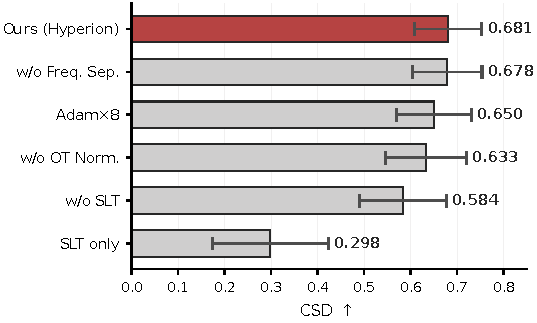
\includegraphics[width=0.48\linewidth]{fig/figure/fig1_ablation.pdf}
  \caption{%
    Component ablation CSD scores (40-sample subset, 8 styles $\times$ 5 prompts,
    seed~43).
    Removing any component degrades performance; the SLT pre-alignment step
    (w/o SLT, CSD~$=0.584$) and doubly-stochastic OT normalization (w/o OT
    Norm., CSD~$=0.633$) show the largest individual drops.
    Hyperion (Ours, CSD~$=0.681$) exceeds Adam$\times$8 (CSD~$=0.650$) at
    $3.0\times$ lower wall-clock cost.%
  }
  \label{fig:ablation_bar}
\end{figure}

% ─────────────────────────────────────────────────────────────────────────────
\section{I2I Style--Content Pareto Scatter}
\label{app:i2i_scatter}

Fig.~\ref{fig:i2i_scatter} plots every I2I method in the style-fidelity
(CSD,~$\uparrow$) versus content-preservation (CLIP-I,~$\uparrow$) plane on the
$40$-pair subset, making the trade-off behind Table~\ref{tab:i2i} explicit. Our
Hyperion (\textcolor{red}{$\star$}) sits at the high-CSD end of the Pareto
frontier: it attains the strongest style fidelity of all methods while giving up
a controlled amount of content similarity, exactly the operating point an
explicit style-transfer pipeline should target.

The floor methods (Text-only, AdaIN) cluster at the bottom-right---high CLIP-I
but almost no style transfer---while Adam-8 reaches high CSD at a CLIP-I cost
similar to ours but at $2.5\times$ the forward-pass budget. No method occupies
the upper-right corner, confirming that style fidelity and content preservation
are genuinely competing objectives in I2I; the contribution of the Hyperion is
reaching the frontier's high-style end \emph{cheaply}, not escaping the
trade-off. The scatter uses the same generation and evaluation configuration as
Table~\ref{tab:i2i} (Sec.~\ref{app:repro}).

\begin{figure}[t]
  \centering
  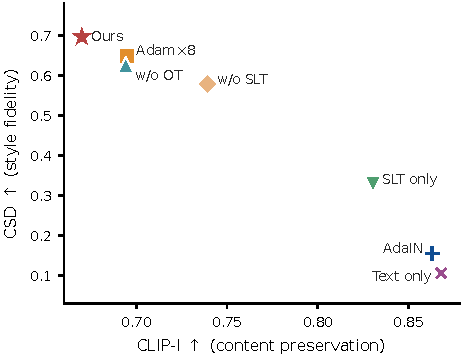
\includegraphics[width=0.52\linewidth]{fig/figure/fig7_i2i_ablation.pdf}
  \caption{%
    I2I style fidelity (CSD, $\uparrow$) vs.\ content preservation (CLIP-I, $\uparrow$)
    scatter plot.
    Hyperion (Ours, \textcolor{red}{$\star$}) anchors the high-CSD end of the
    Pareto frontier, achieving the strongest style fidelity while trading away
    some content preservation (lower CLIP-I).
    AdaIN and Text-only barely transfer style (bottom right);
    SLT-only preserves content but lacks texture;
    Adam-8 also reaches high CSD at the cost of CLIP-I.%
  }
  \label{fig:i2i_scatter}
\end{figure}

% ─────────────────────────────────────────────────────────────────────────────
\section{Cross-Backbone Generalization: FLUX.1-dev}
\label{app:flux1dev}

We validate that our Hyperion pipeline generalizes to a second MM-DiT backbone, FLUX.1-dev~\cite{flux2024}, without any hyperparameter changes.
FLUX.1-dev is a 12B-parameter flow-matching transformer sharing the same MM-DiT architecture (double + single stream blocks) as Klein~9B used in the main paper.
We run the identical Hyperion pipeline on the same 40-sample evaluation subset (8 styles $\times$ 5 prompts, \texttt{sty} 00/10/14/20/27/28/33/38).

\begin{table}[h]
  \centering
  \caption{%
    Cross-backbone generalization: Hyperion on FLUX.1-dev vs.\ Klein~9B (same 40-sample subset).
    All hyperparameters identical; no backbone-specific tuning.%
  }
  \label{tab:flux1dev}
  \footnotesize
  \begin{tabular}{lcc}
    \toprule
    Backbone & CSD~$\uparrow$ & CLIP-T~$\uparrow$ \\
    \midrule
    Klein~9B (main)    & 0.681 & 0.274 \\
    FLUX.1-dev         & \textbf{0.719} & \textbf{0.291} \\
    \bottomrule
  \end{tabular}
\end{table}

FLUX.1-dev achieves higher CSD ($+5.6\%$) and higher CLIP-T ($+1.7$~pp) than Klein~9B on the same prompt--style pairs.
The improvement is consistent with FLUX.1-dev's larger capacity: a stronger backbone produces better style transfer with any guidance signal.
Crucially, the Hyperion pipeline requires \emph{no modification} to transfer to a different MM-DiT backbone, confirming that its design is generic within the MM-DiT family.

% ─────────────────────────────────────────────────────────────────────────────
\section{Supplementary Perceptual Metrics}
\label{app:supp_metrics}

To corroborate the CSD-based comparisons and address potential metric-hacking concerns, we evaluate two additional perceptual metrics on the same 40-sample ablation subset ($8$ styles $\times$ $5$ prompts): \textbf{DINO-style similarity} (DINOv2~\cite{oquab2024dinov2} CLS-token cosine similarity between output and style image) and \textbf{Gram distance} (mean Frobenius distance of VGG-19 Gram matrices, lower is better style transfer).
We also compute \textbf{layout leakage} (DINO patch-token spatial self-similarity Pearson correlation between output and style, measuring how much the style image's spatial layout appears in the output).

\begin{table}[h]
  \centering
  \caption{%
    Supplementary perceptual metrics on the 40-sample ablation subset.
    DINO-style: DINOv2 CLS cosine similarity to style image ($\uparrow$).
    Gram distance: mean VGG-19 Gram Frobenius distance to style ($\downarrow$).
    Layout leakage: DINO spatial self-similarity correlation with style ($\uparrow$ means less leakage suppression).
    Boldface = best (excluding LRS-off which is a variant of Ours).%
  }
  \label{tab:supp_metrics}
  \footnotesize
  \begin{tabular}{lccc}
    \toprule
    Method & DINO-style~$\uparrow$ & Gram-dist~$\downarrow$ & Layout-leak~$\uparrow$ \\
    \midrule
    \textbf{Ours (Hyperion)} & \textbf{0.1548} & \textbf{2.731} & 0.3354 \\
    StyleShot               & 0.1280 & 3.541 & 0.3180 \\
    USO                     & 0.1092 & 3.681 & 0.3221 \\
    CSGO                    & 0.1324 & 5.589 & 0.3408 \\
    IP-Adapter              & 0.0975 & 4.297 & 0.3540 \\
    \midrule
    Ours w/o LRS            & 0.1639 & 2.536 & 0.3413 \\
    \bottomrule
  \end{tabular}
\end{table}

\paragraph{Corroboration of CSD ranking}
Across all five methods, Ours ranks \emph{first} on both DINO-style similarity
($0.1548$) and Gram distance ($2.731$), consistent with the CSD ranking
(Table~\ref{tab:percat}); the trained adapters CSGO and IP-Adapter, despite
strong color transfer, score markedly worse on Gram distance ($5.589$, $4.297$)
and exhibit the highest layout leakage ($0.341$, $0.354$).
This consistency across four independent metrics---CSD, DINO-style similarity, Gram distance, and layout leakage---provides strong evidence that our advantage in CSD reflects genuine style fidelity rather than metric-specific optimization.

\paragraph{LRS layout suppression}
Comparing Ours vs.\ Ours w/o LRS (a paired $n{=}40$ test) quantifies the effect of Layout Residual Suppression:
layout leakage increases by $+0.0059$ ($t = +2.84$, $27/40$ pairs, $p < 0.01$) when LRS is \emph{disabled},
and Gram distance \emph{decreases} by $0.196$ ($t = -4.89$, $33/40$ pairs, $p < 0.001$).
This confirms that LRS statistically significantly reduces the leakage of the style image's spatial layout into the output, while accepting a modest increase in Gram distance (i.e., slightly less texture duplication).
DINO-style similarity shows no significant difference ($t = +1.14$, n.s.),
indicating that LRS's suppression of layout does not harm overall style perception.
Fig.~\ref{fig:lrs_demo} shows the effect qualitatively.

\begin{figure}[tbp]
  \centering
  \begin{subfigure}{\linewidth}
    \centering
    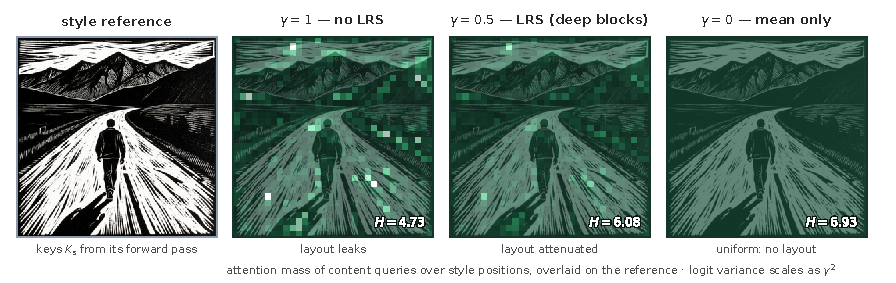
\includegraphics{fig/figure/fig18a_lrs_mech_v2.pdf}
    \caption{Mechanism, measured on real tensors: attention mass that
    content queries place on style positions (deep self-attention layer,
    Klein-9B, overlaid on the reference; $H$ = mean attention entropy in
    nats). With full keys ($\gamma{=}1$) the mass concentrates on the
    reference's layout---the leak; LRS ($\gamma{=}0.5$ in deep blocks)
    attenuates exactly this component, the logit variance scaling as
    $\gamma^2$ (Eq.~\ref{eq:lrs_var}); at $\gamma{=}0$ the distribution is
    uniform ($H{=}\ln 1024{=}6.93$).}
    \label{fig:lrs_mech}
  \end{subfigure}
  \\[6pt]
  \begin{subfigure}{\linewidth}
    \centering
    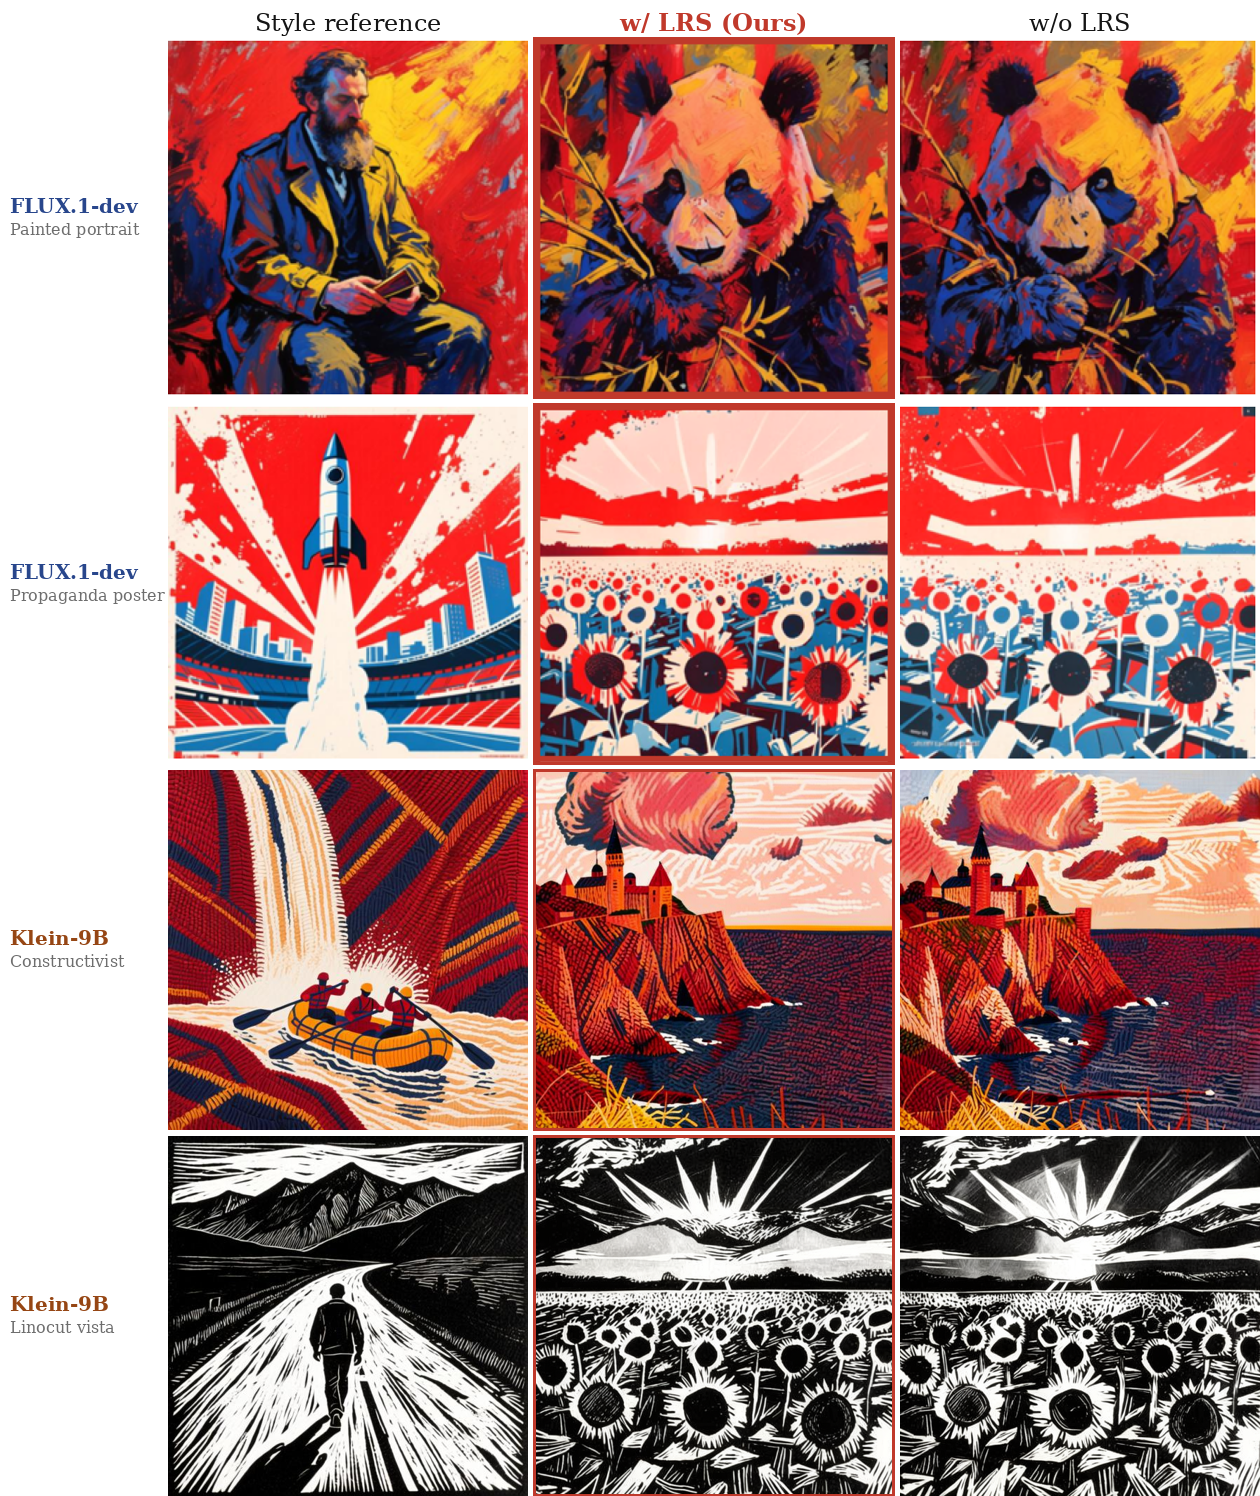
\includegraphics[width=0.62\linewidth]{figures_hires/fig18_lrs_demo.png}
    \caption{Representative LRS effect on strong-composition styles, shown
      \emph{across backbones}: \emph{rows 1--2}, FLUX.1-dev (painted portrait,
      content ``a panda''; and a propaganda poster); \emph{rows 3--4}, Klein-9B
      (constructivist poster, content ``a castle''; and a linocut vista).
      \emph{Columns}: style reference; \textbf{w/ LRS (Ours)}; w/o LRS. Without
      LRS the style's dominant composition re-emerges behind the subject---the
      portrait's face re-appears behind the panda, and radiating/diagonal
      structures intensify---and LRS attenuates this layout residual on
      \emph{both} backbones. The effect is \emph{localized and most visible for
      styles with a dominant repeating composition}; for many styles the change
      is subtle.}
    \label{fig:lrs_demo_qual}
  \end{subfigure}
  \caption{Layout Residual Suppression (LRS): \textbf{(a)} mechanism and
    \textbf{(b)} representative effect. The \emph{primary} evidence for LRS is the
    paired layout-leak test in the text ($+0.0059$ reduction, $t{=}2.84$,
    $p<0.01$, $27/40$ pairs), corroborated by these examples.}
  \label{fig:lrs_demo}
\end{figure}

% ─────────────────────────────────────────────────────────────────────────────
\section{Layout Residual Suppression: Leakage Bound}
\label{app:lrs_proof}

We make precise the claim of \cref{sec:method:lrs} that attenuating the style
residual suppresses layout leakage. Fix a content query $q_i$ and a layer
$\ell$ (we drop $\ell$). Under LRS the style key/value tensors are
$K_s'=\mu_K+\gamma R_K$ and $V_s'=\mu_V+\gamma R_V$, with
$\mu=\tfrac1L\sum_j(\cdot)_j$ the token mean and $R=(\cdot)-\mu$ the
position-specific residual ($\sum_j R_j=0$). The attention output is
$o_i=\sum_j a_{ij}V_{s,j}'$ with $a_{ij}=\mathrm{softmax}_j(q_i^\top K_{s,j}'/\sqrt d)$.

\paragraph{Layout leakage}
Define the \emph{layout-agnostic} output as the one obtained if the query
attended uniformly, $\bar a=1/L$, and define the layout leakage as the
position-dependent deviation
$\mathcal{L}_i \;=\; o_i-\sum_j \bar a\,V_{s,j}' \;=\; \sum_j (a_{ij}-\bar a)\,V_{s,j}'$.
Because $V_{s,j}'=\mu_V+\gamma R_{V,j}$ and $\sum_j(a_{ij}-\bar a)=0$, the mean
term cancels and
\begin{equation}
  \mathcal{L}_i \;=\; \gamma \sum_j (a_{ij}-\bar a)\,R_{V,j}.
  \label{eq:leak_def}
\end{equation}

\paragraph{Proposition (quadratic suppression)}
Let $q_{\max}=\max_i\|q_i\|$ and $\rho_K=\max_j\|R_{K,j}\|$,
$\rho_V=(\tfrac1L\sum_j\|R_{V,j}\|^2)^{1/2}$. Then
\begin{equation}
  \|\mathcal{L}_i\| \;\le\; \frac{q_{\max}\,\rho_K\,\rho_V}{\sqrt d}\;\gamma^2
  \;+\; O(\gamma^3).
  \label{eq:leak_bound}
\end{equation}
Hence layout leakage vanishes \emph{quadratically} as $\gamma\to0$, while the
global style statistics in $\mu_V$ are retained exactly.

\paragraph{Proof}
The logits are $s_{ij}=(q_i^\top\mu_K+\gamma\,q_i^\top R_{K,j})/\sqrt d$. The
first part is constant in $j$ and cancels in the softmax, so
$a_{ij}=\mathrm{softmax}_j(\gamma\,q_i^\top R_{K,j}/\sqrt d)$. A first-order
expansion of the softmax about the uniform point ($\gamma{=}0$, where
$a_{ij}=\bar a$) gives
$a_{ij}-\bar a=\frac{\gamma}{\sqrt d}\,\bar a\big(q_i^\top R_{K,j}-\textstyle\frac1L\sum_k q_i^\top R_{K,k}\big)+O(\gamma^2)
=\frac{\gamma}{\sqrt d}\,\bar a\,q_i^\top R_{K,j}+O(\gamma^2)$,
using $\sum_k R_{K,k}=0$. Substituting into \cref{eq:leak_def},
$\mathcal{L}_i=\frac{\gamma^2}{\sqrt d}\,\bar a\sum_j (q_i^\top R_{K,j})R_{V,j}+O(\gamma^3)$.
By Cauchy--Schwarz, $\|\sum_j(q_i^\top R_{K,j})R_{V,j}\|\le \|q_i\|\big(\sum_j\|R_{K,j}\|\,\|R_{V,j}\|\big)\le L\,q_{\max}\rho_K\rho_V$, and $\bar a=1/L$, which gives \cref{eq:leak_bound}. $\qed$

The two factors of $\gamma$ have distinct origins: one from the attention weights
becoming position-selective (through $R_K$), one from the injected values
themselves carrying layout (through $R_V$). Suppressing either alone would give
only linear decay; LRS attenuates both, yielding the $\gamma^2$ rate. This is the
analytic counterpart of the $\gamma^2$ logit-variance identity
(\cref{eq:lrs_var}) and of the small, significant layout-leak reduction measured
in \cref{tab:supp_metrics}.

% ─────────────────────────────────────────────────────────────────────────────
\section{Additional Metrics: LPIPS, ArtFID, and Texture Coherence}
\label{app:newmetrics}

The main paper leads with CSD but always reads it jointly with CLIP-T/CLIP-I and
corroborates it with three perceptual metrics (Sec.~\ref{app:supp_metrics}). For
completeness we add three further views, all computed on the
\emph{already-generated} images with no regeneration: LPIPS and ArtFID for the
I2I setting, and an output-space texture-coherence analysis that mirrors the
update-space diagnostic $\rho$.

\subsection{LPIPS and ArtFID (I2I)}
LPIPS~\cite{zhang2018unreasonable} and ArtFID~\cite{wright2022artfid} are the
standard content- and style-aware metrics for image-conditioned style transfer;
both require a content image and therefore apply to our I2I setting (not T2I).
Table~\ref{tab:newmetrics_i2i} reports them on the $40$-pair I2I subset.
\textbf{LPIPS} is the AlexNet perceptual distance between output and content
image (lower $=$ more content preserved); consistent with CLIP-I
(Table~\ref{tab:i2i}), the strongly-stylising methods (Ours, Adam-8) diverge more
from the content photo than the near-pass-through floors (AdaIN, Text-only),
reflecting the same style--content trade-off rather than a defect, and Ours and
Adam-8 are near-tied ($0.687$ vs.\ $0.675$).
\textbf{ArtFID}~$=(1+\mathrm{LPIPS})(1+\mathrm{FID}_{\text{style}})$ combines
content distance with a style-distribution distance: our method attains the
\emph{best} (lowest) $\mathrm{FID}_{\text{style}}$, and its ArtFID is
statistically tied with the AdaIN floor ($10.8$ vs.\ $10.7$). The floor's low
ArtFID is an artifact of its minimal content change (lowest LPIPS), not of style
transfer---it barely stylises (CSD~$0.155$ vs.\ Ours~$0.696$)---so we read
ArtFID jointly with CSD/STM rather than in isolation.

\paragraph{Small-sample FID}
The $\mathrm{FID}_{\text{style}}$ term is a dataset-level FID between each
method's stylised outputs and the pool of style references. With only $40$
outputs per method, the default $2048$-dimensional Inception covariance is
rank-deficient and inflates FID by an order of magnitude; we therefore use the
$64$-dimensional Inception feature (matching Table~\ref{tab:i2i_ext}), which is
appropriate at $n{=}40$ and yields calibrated, stable values.

\begin{table}[t]
  \centering
  \caption{Supplementary I2I metrics on the $40$-pair subset. LPIPS (AlexNet) is
           distance to the content image; $\mathrm{FID}_{\text{style}}$ and ArtFID
           use the $64$-d Inception feature (appropriate at $n{=}40$;
           cf.\ Table~\ref{tab:i2i_ext}). All lower $=$ better; \textbf{bold} $=$
           best (ArtFID: the AdaIN floor's value is a minimal-change artifact,
           see text).}
  \label{tab:newmetrics_i2i}
  \footnotesize
  \begin{tabular}{lccc}
    \toprule
    Method & LPIPS$\downarrow$ & $\mathrm{FID}_{\text{style}}\downarrow$ & ArtFID$\downarrow$ \\
    \midrule
    \textbf{Ours (Hyperion)} & $0.687$ & $\mathbf{5.4}$ & $10.8$ \\
    Adam-8                 & $0.675$ & $6.5$ & $12.6$ \\
    AdaIN (floor)          & $0.514$ & $6.1$ & $\mathbf{10.7}$ \\
    Text-only              & $0.500$ & $6.7$ & $11.6$ \\
    \bottomrule
  \end{tabular}
\end{table}

\subsection{Output-Space Texture Coherence}
The output-space texture-coherence analysis---texture energy and structure-tensor
orientation coherence, the pixel-space analogue of the spatial-neighbor cosine
$\rho$---is promoted to the main paper (Sec.~\ref{sec:exp:texcoh},
Table~\ref{tab:texcoh}), where both measures peak for our method and track CSD
across the five pipeline variants at Pearson $r{=}{+}0.97$ (energy) and
$r{=}{+}0.88$ (coherence). We record one methodological pitfall for reproducers:
a naive adjacent-patch residual \emph{similarity} score anti-correlates with CSD
($r{=}{-}0.97$) because it rewards the smoothness of weakly textured outputs; the
energy and orientation measures avoid this inversion.

% ─────────────────────────────────────────────────────────────────────────────
\section{Comparison with Trained Style Transfer Methods}
\label{app:trained_baselines}

Fig.~\ref{fig:trained_baselines} provides qualitative comparisons between our
Hyperion pipeline and four representative trained style-transfer methods:
StyleShot~\cite{gao2024styleshot}, USO~\cite{wu2025uso},
CSGO~\cite{xing2024csgo}, and IP-Adapter~\cite{ipadapter2023}.
To stress-test breadth, all methods are run on the same content prompt
(``A panda eat bamboo'') across \emph{21 diverse style families} spanning the
full medium gamut---line/ink (linocut, manga, ink-storybook, Chinese ink,
ukiyo-e), painterly (oil impasto, impasto collage), 3D/sculptural (bronze
bas-relief, low-poly voxel), pixel/digital (pixel art, cyberpunk neon),
textile/craft (embroidery, gold mosaic, stained glass), illustration
(anime cel, graffiti, steampunk), and print/poster (screenprint, pop halftone,
propaganda).
Trained methods often produce strong color transfer but tend toward either
layout leakage (USO, CSGO) or mode collapse toward the style image composition
(IP-Adapter), and more often match hue than medium on structured styles; our
method reproduces the medium-defining structure across the gamut.
Table~\ref{tab:percat} reports the corresponding per-family CSD: our
% 十修: 0.655→0.657 — tab:percat Ours column realigned to the 5-prompt
% (p0--p4) footing shared with the baselines (C15 方案 a).
training-free Hyperion leads on \textbf{19 of 21} families (mean CSD $0.657$
vs.\ the strongest trained adapter CSGO at $0.506$, then $0.489$ StyleShot,
$0.454$ USO, $0.420$ IP-Adapter),
the two exceptions being manga and anime, where IP-Adapter---tuned for
character imagery---scores higher. The full per-family CSD table is promoted to
the main text (Table~\ref{tab:percat}); the qualitative companion spans the
three panels below (Figs.~\ref{fig:trained_baselines}--\ref{fig:trained_baselines_c}),
each showing seven of the 21 families across all six methods.

\paragraph{Reading the comparison}
Each row places the style reference beside our training-free Hyperion output and
the four trained adapters under the identical prompt, so a single glance
isolates \emph{what each method does with the same style cue}. The recurring
pattern is that the trained adapters reproduce the reference's \emph{palette}
but flatten its \emph{medium}: USO and CSGO frequently import the style image's
global composition (layout leakage), IP-Adapter collapses toward the style
subject, and StyleShot retains hue while smoothing away the defining surface
structure. Our method instead reconstructs the medium-defining geometry---gouged
linocut grooves, palette-knife impasto ridges, embossed bronze relief, blocky
pixel dithering, square mosaic tesserae, faceted low-poly planes, and dense ink
hatching---while keeping the prompted subject (a panda) intact.

These are exactly the cases that the per-family CSD in Table~\ref{tab:percat}
quantifies: the structured, medium-heavy families (relief, mosaic, voxel,
impasto, linocut) are where our margin over the trained adapters is largest,
whereas the two exceptions (manga, anime) are character-illustration styles for
which IP-Adapter's character tuning is well matched. All tiles are generated at
the configuration of Sec.~\ref{app:repro:baselines}; the displayed \textbf{Ours}
tiles are the best of six seeds $\{43\text{--}48\}$ selected jointly on CSD and
CLIP-T, while every number in Table~\ref{tab:percat} uses the fixed seed~43.

\begin{figure}[t]
  \centering
  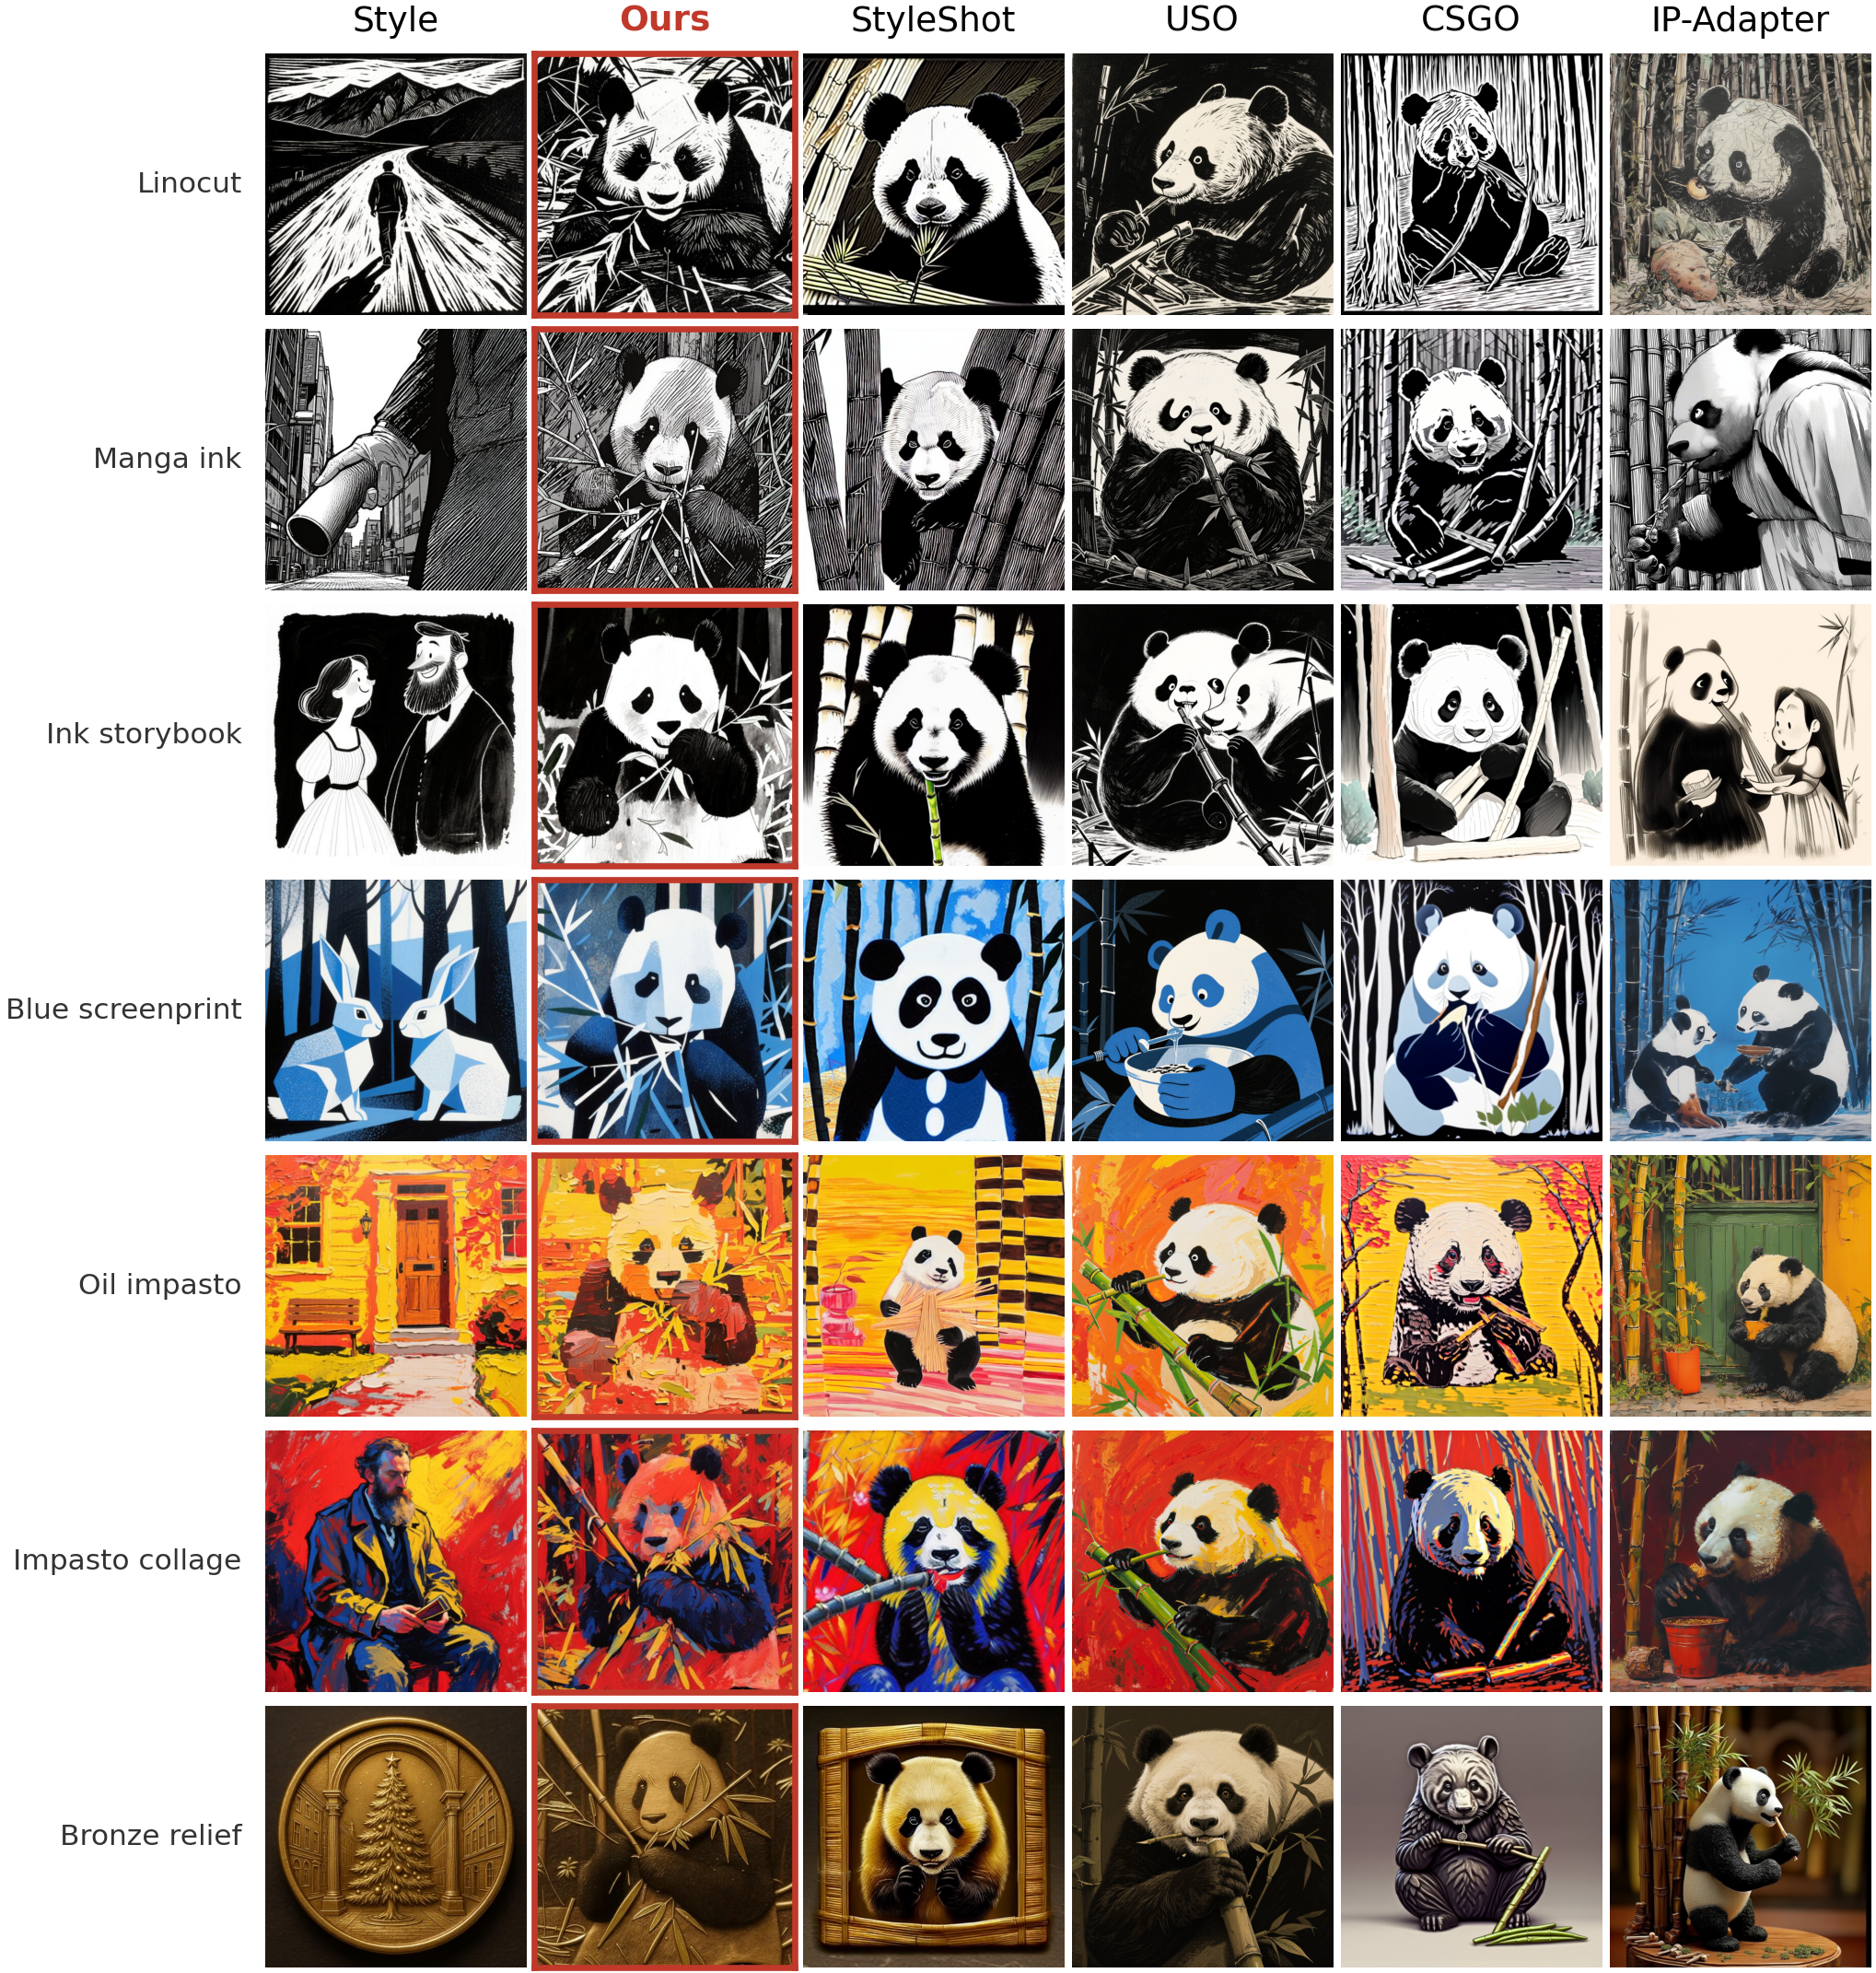
\includegraphics[width=\linewidth]{figures_hires/fig16a_diverse_supp.png}
  \caption{%
    Qualitative comparison with trained baselines, \textbf{families 1--7 of 21}
    (prompt: ``A panda eat bamboo''); continued in
    Figs.~\ref{fig:trained_baselines_b}--\ref{fig:trained_baselines_c}.
    \emph{Rows}: style family (labelled at left).
    \emph{Columns}: style reference, \textbf{Ours} (Hyperion), StyleShot, USO,
    CSGO, IP-Adapter.
    Our training-free method reproduces medium-defining structure---gouged
    relief, palette-knife facets, embossed metal, dense ink hatching---where
    trained adapters collapse to color-only shifts, without any per-style
    optimization.
    Displayed \textbf{Ours} tiles are the best of six seeds $\{43\text{--}48\}$;
    all quantitative tables (Table~\ref{tab:percat}) use the fixed seed~43.%
  }
  \label{fig:trained_baselines}
\end{figure}

\begin{figure}[t]
  \centering
  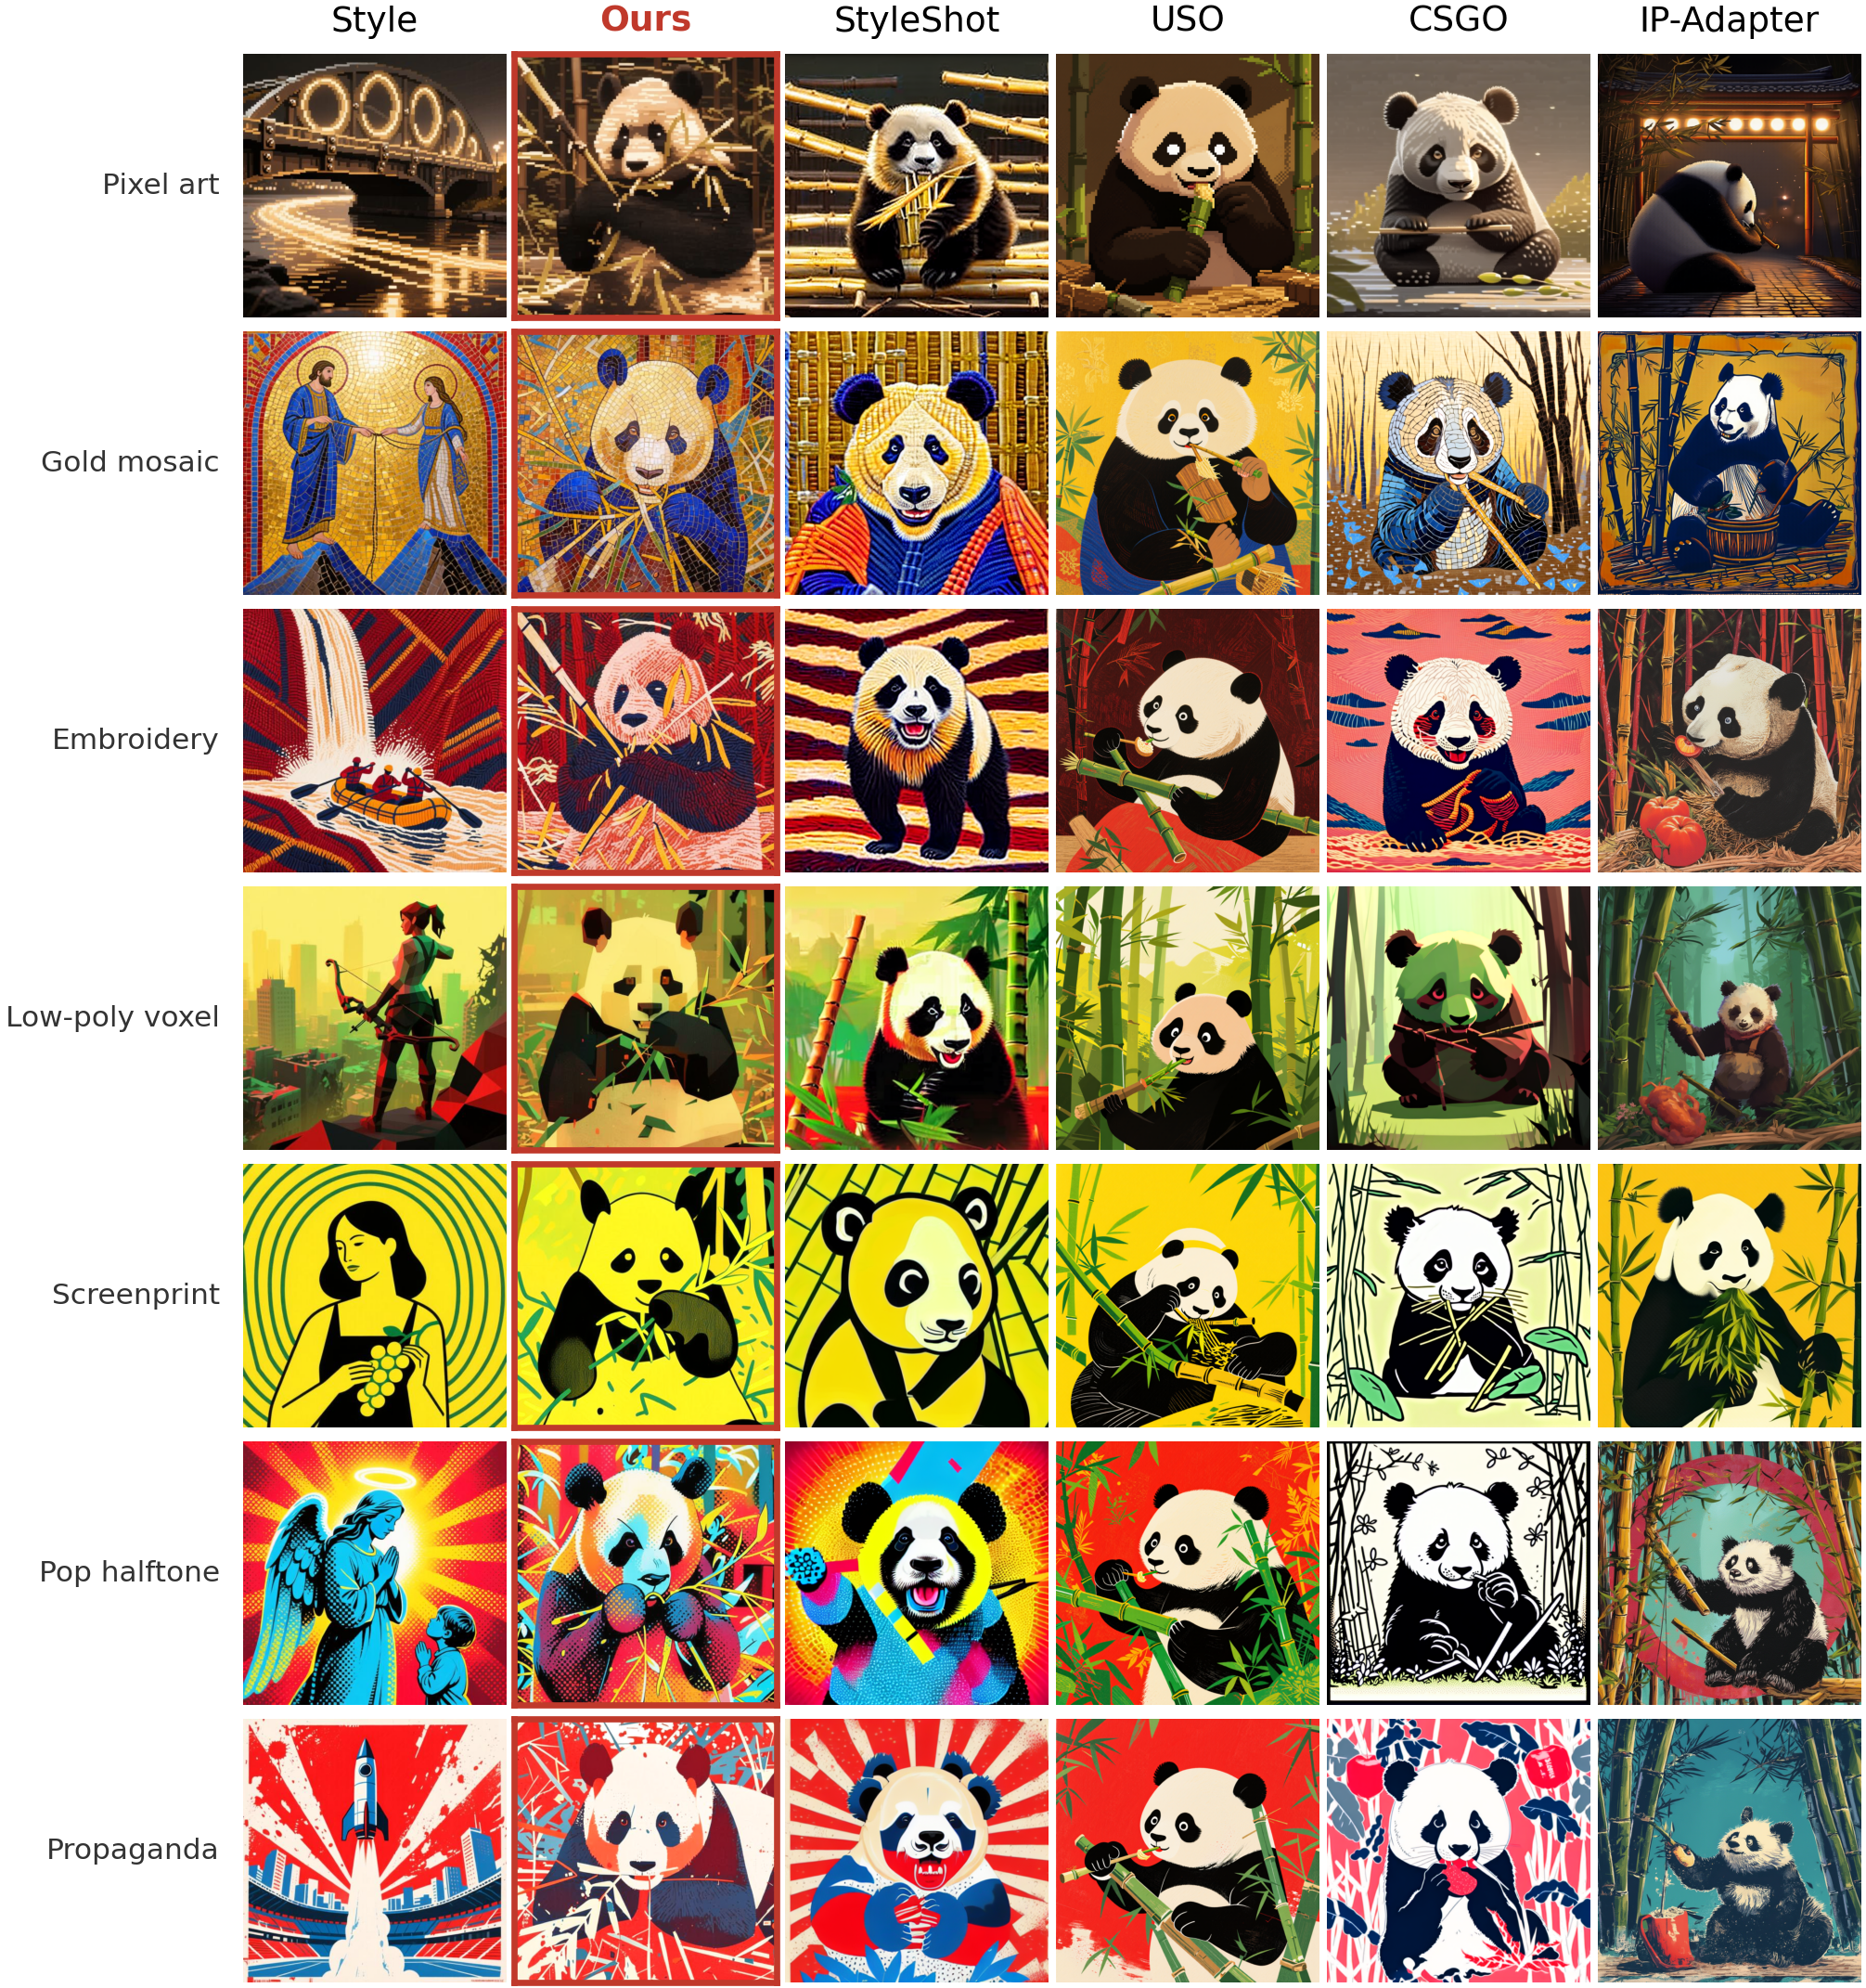
\includegraphics[width=\linewidth]{figures_hires/fig16b_diverse_supp.png}
  \caption{%
    Trained-baseline comparison, \textbf{families 8--14 of 21}
    (continued from Fig.~\ref{fig:trained_baselines}; same columns and protocol).
    Structured media (mosaic, voxel, impasto, pixel) are where our margin over
    the trained adapters is largest; the trained methods preserve hue but flatten
    surface geometry.%
  }
  \label{fig:trained_baselines_b}
\end{figure}

\begin{figure}[t]
  \centering
  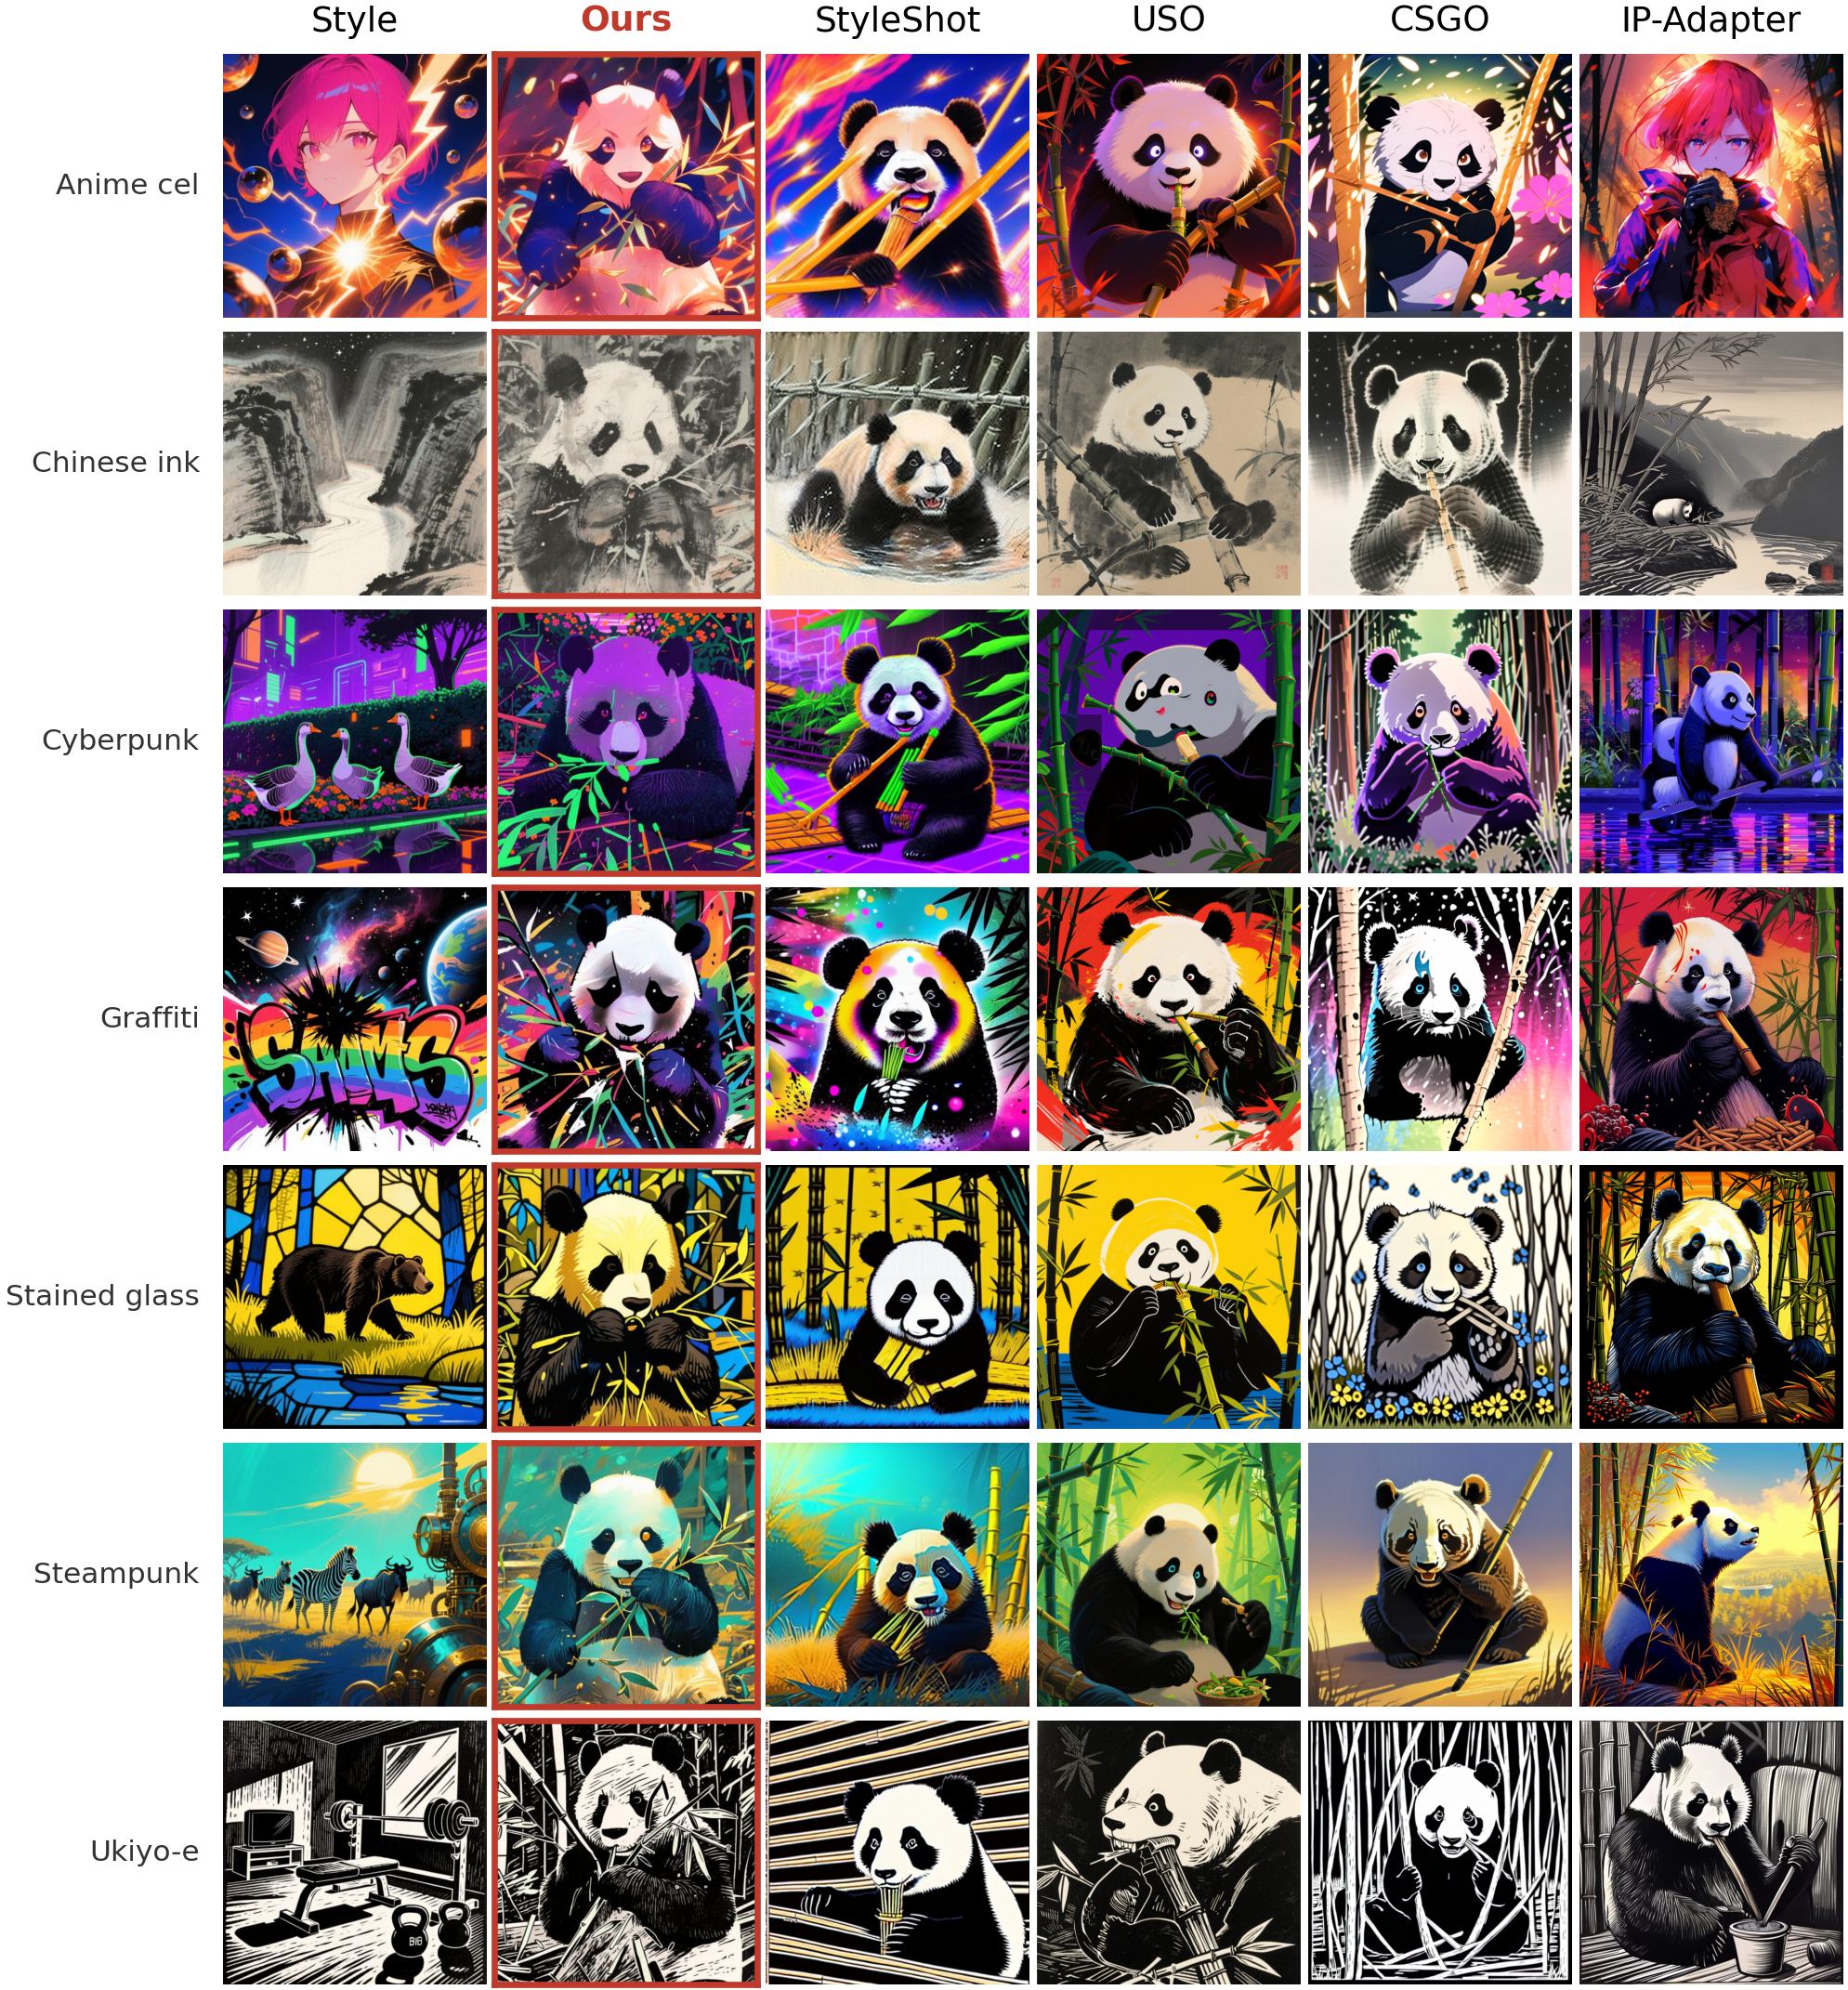
\includegraphics[width=\linewidth]{figures_hires/fig16c_diverse_supp.png}
  \caption{%
    Trained-baseline comparison, \textbf{families 15--21 of 21}
    (continued from Figs.~\ref{fig:trained_baselines}--\ref{fig:trained_baselines_b}).
    Includes the two families (anime, manga in the earlier panel) on which the
    character-tuned IP-Adapter edges ahead; across all 21 families our
    training-free method still leads on 19 (Table~\ref{tab:percat}).%
  }
  \label{fig:trained_baselines_c}
\end{figure}

% ─────────────────────────────────────────────────────────────────────────────
\section{Additional Qualitative Comparisons}
\label{app:qualitative}

Fig.~\ref{fig:qualitative} extends the main-paper qualitative comparison to five
additional style references under a fixed prompt, placing all seven pipeline
variants side by side so that the contribution of each stage is visible on the
same content. Reading left to right, attention injection yields only a faint hue
wash; SLT-only matches the reference palette but leaves the surface flat;
removing SLT or the OT normalisation desaturates the colour and destabilises the
attention; Adam-8 recovers brushstroke texture but at $2.5\times$ the
forward-pass cost; and our Hyperion attains the same rich texture with the subject
cleanly preserved. The progression is the qualitative counterpart of the
component ablation in Fig.~\ref{fig:ablation_bar}.

These examples also localise the failure modes. The injection and SLT-only
columns lose texture uniformly across the image, whereas the \emph{w/o OT-norm}
column shows patches of colour collapse where unconstrained transport
over-commits mass to a few style tokens---precisely the mode collapse that the
doubly-stochastic Sinkhorn constraint is designed to prevent
(Sec.~\ref{sec:method:slt}). All tiles use the configuration of
Sec.~\ref{app:repro}.

% 十修排版: fig:qualitative 与 fig:ablation_qual 合并为同一浮动页（一个
% figure 环境内两个 \caption，编号与 \ref 不变），消除各自独占页的下半空白。
\begin{figure}[!tp]
  \centering
  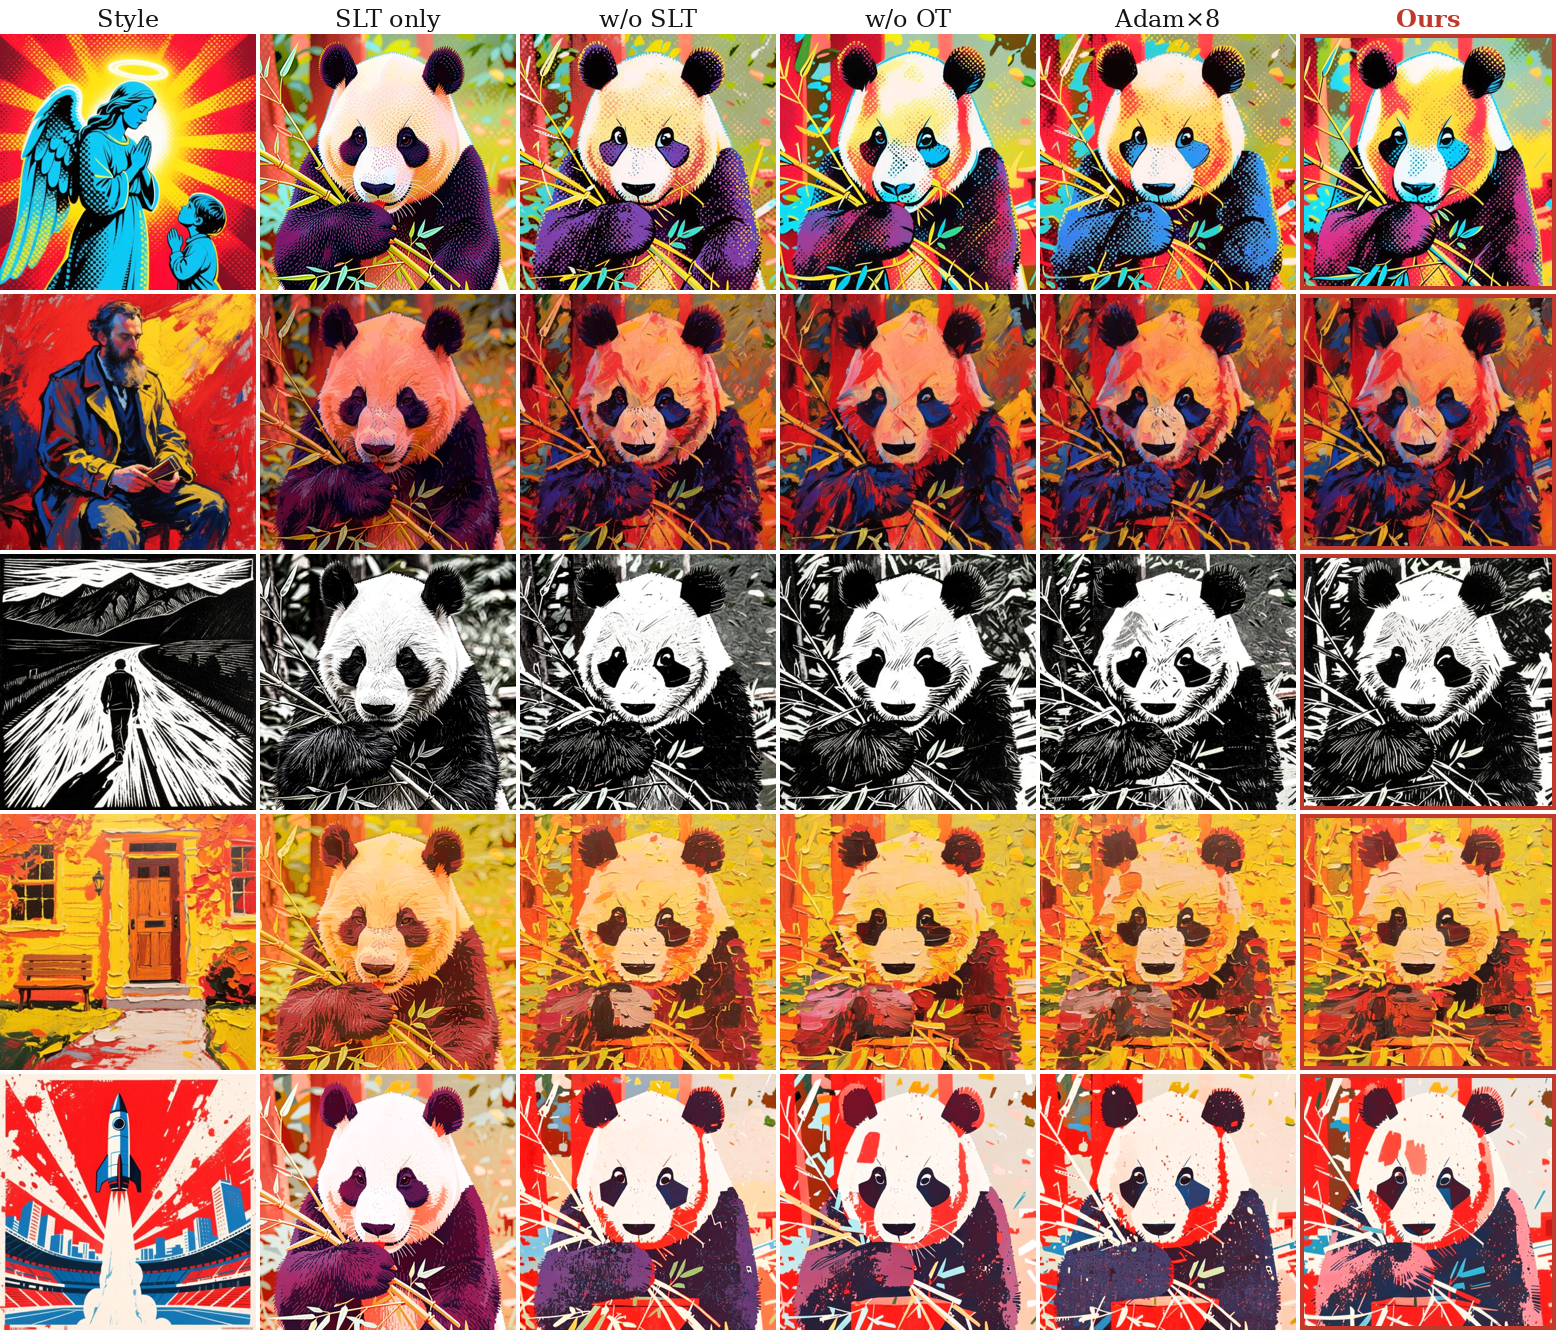
\includegraphics[width=\linewidth]{figures_hires/fig9_qualitative_t2i.png}
  \caption{%
    Additional qualitative comparison across five style references
    (content prompt: ``A panda eating bamboo'').
    \emph{Columns}: style reference, SLT-only, w/o SLT (Adam-only),
    w/o OT-norm, Adam-8, \textbf{Ours} (Hyperion).
    SLT-only matches colors but lacks painterly structure; removing SLT or
    OT-normalization degrades color fidelity and attention quality;
    Adam-8 generates brushstrokes at high cost;
    \textbf{Ours} achieves rich brushstroke texture with intact subject
    placement at $2.5\times$ lower forward-pass cost.%
  }
  \label{fig:qualitative}

  \vspace{2.5ex}
  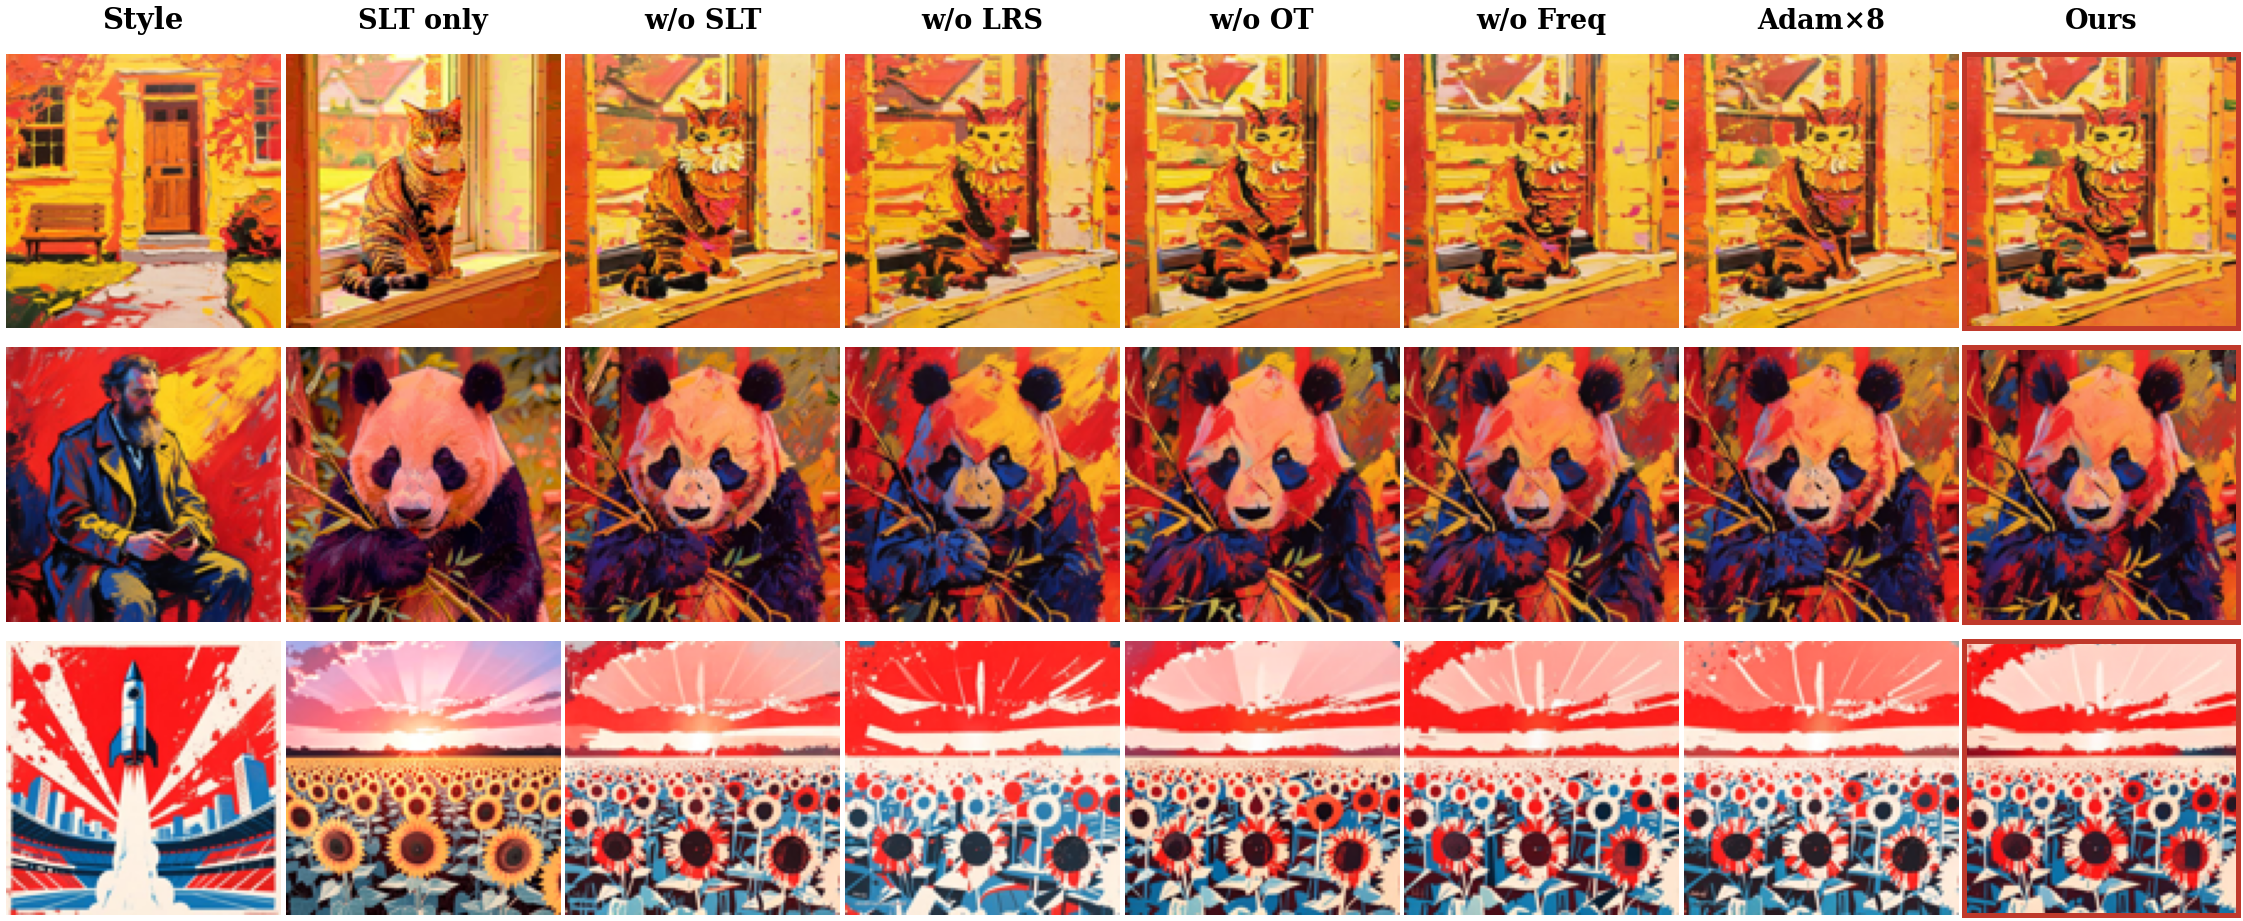
\includegraphics[width=\linewidth]{figures_hires/fig11_qualitative_ablation.png}
  \caption{%
    Visual ablation across three content--style examples (one per row).
    \emph{Columns, left to right}: style reference; SLT-only (color match, no
    brushstroke texture); w/o SLT (texture present but color misaligned);
    w/o LRS (style layout leaks into subject placement); w/o OT Norm.\
    (muddy, mode-collapsed attention); w/o freq.\ boost (slightly softened
    edges); Adam$\times$8 (reference upper bound); \textbf{Ours} (Hyperion,
    matched quality at $2.5\times$ fewer forward passes).
    The per-column effect is consistent across the three examples.%
  }
  \label{fig:ablation_qual}
\end{figure}

\begin{figure}[!tp]
  \centering
  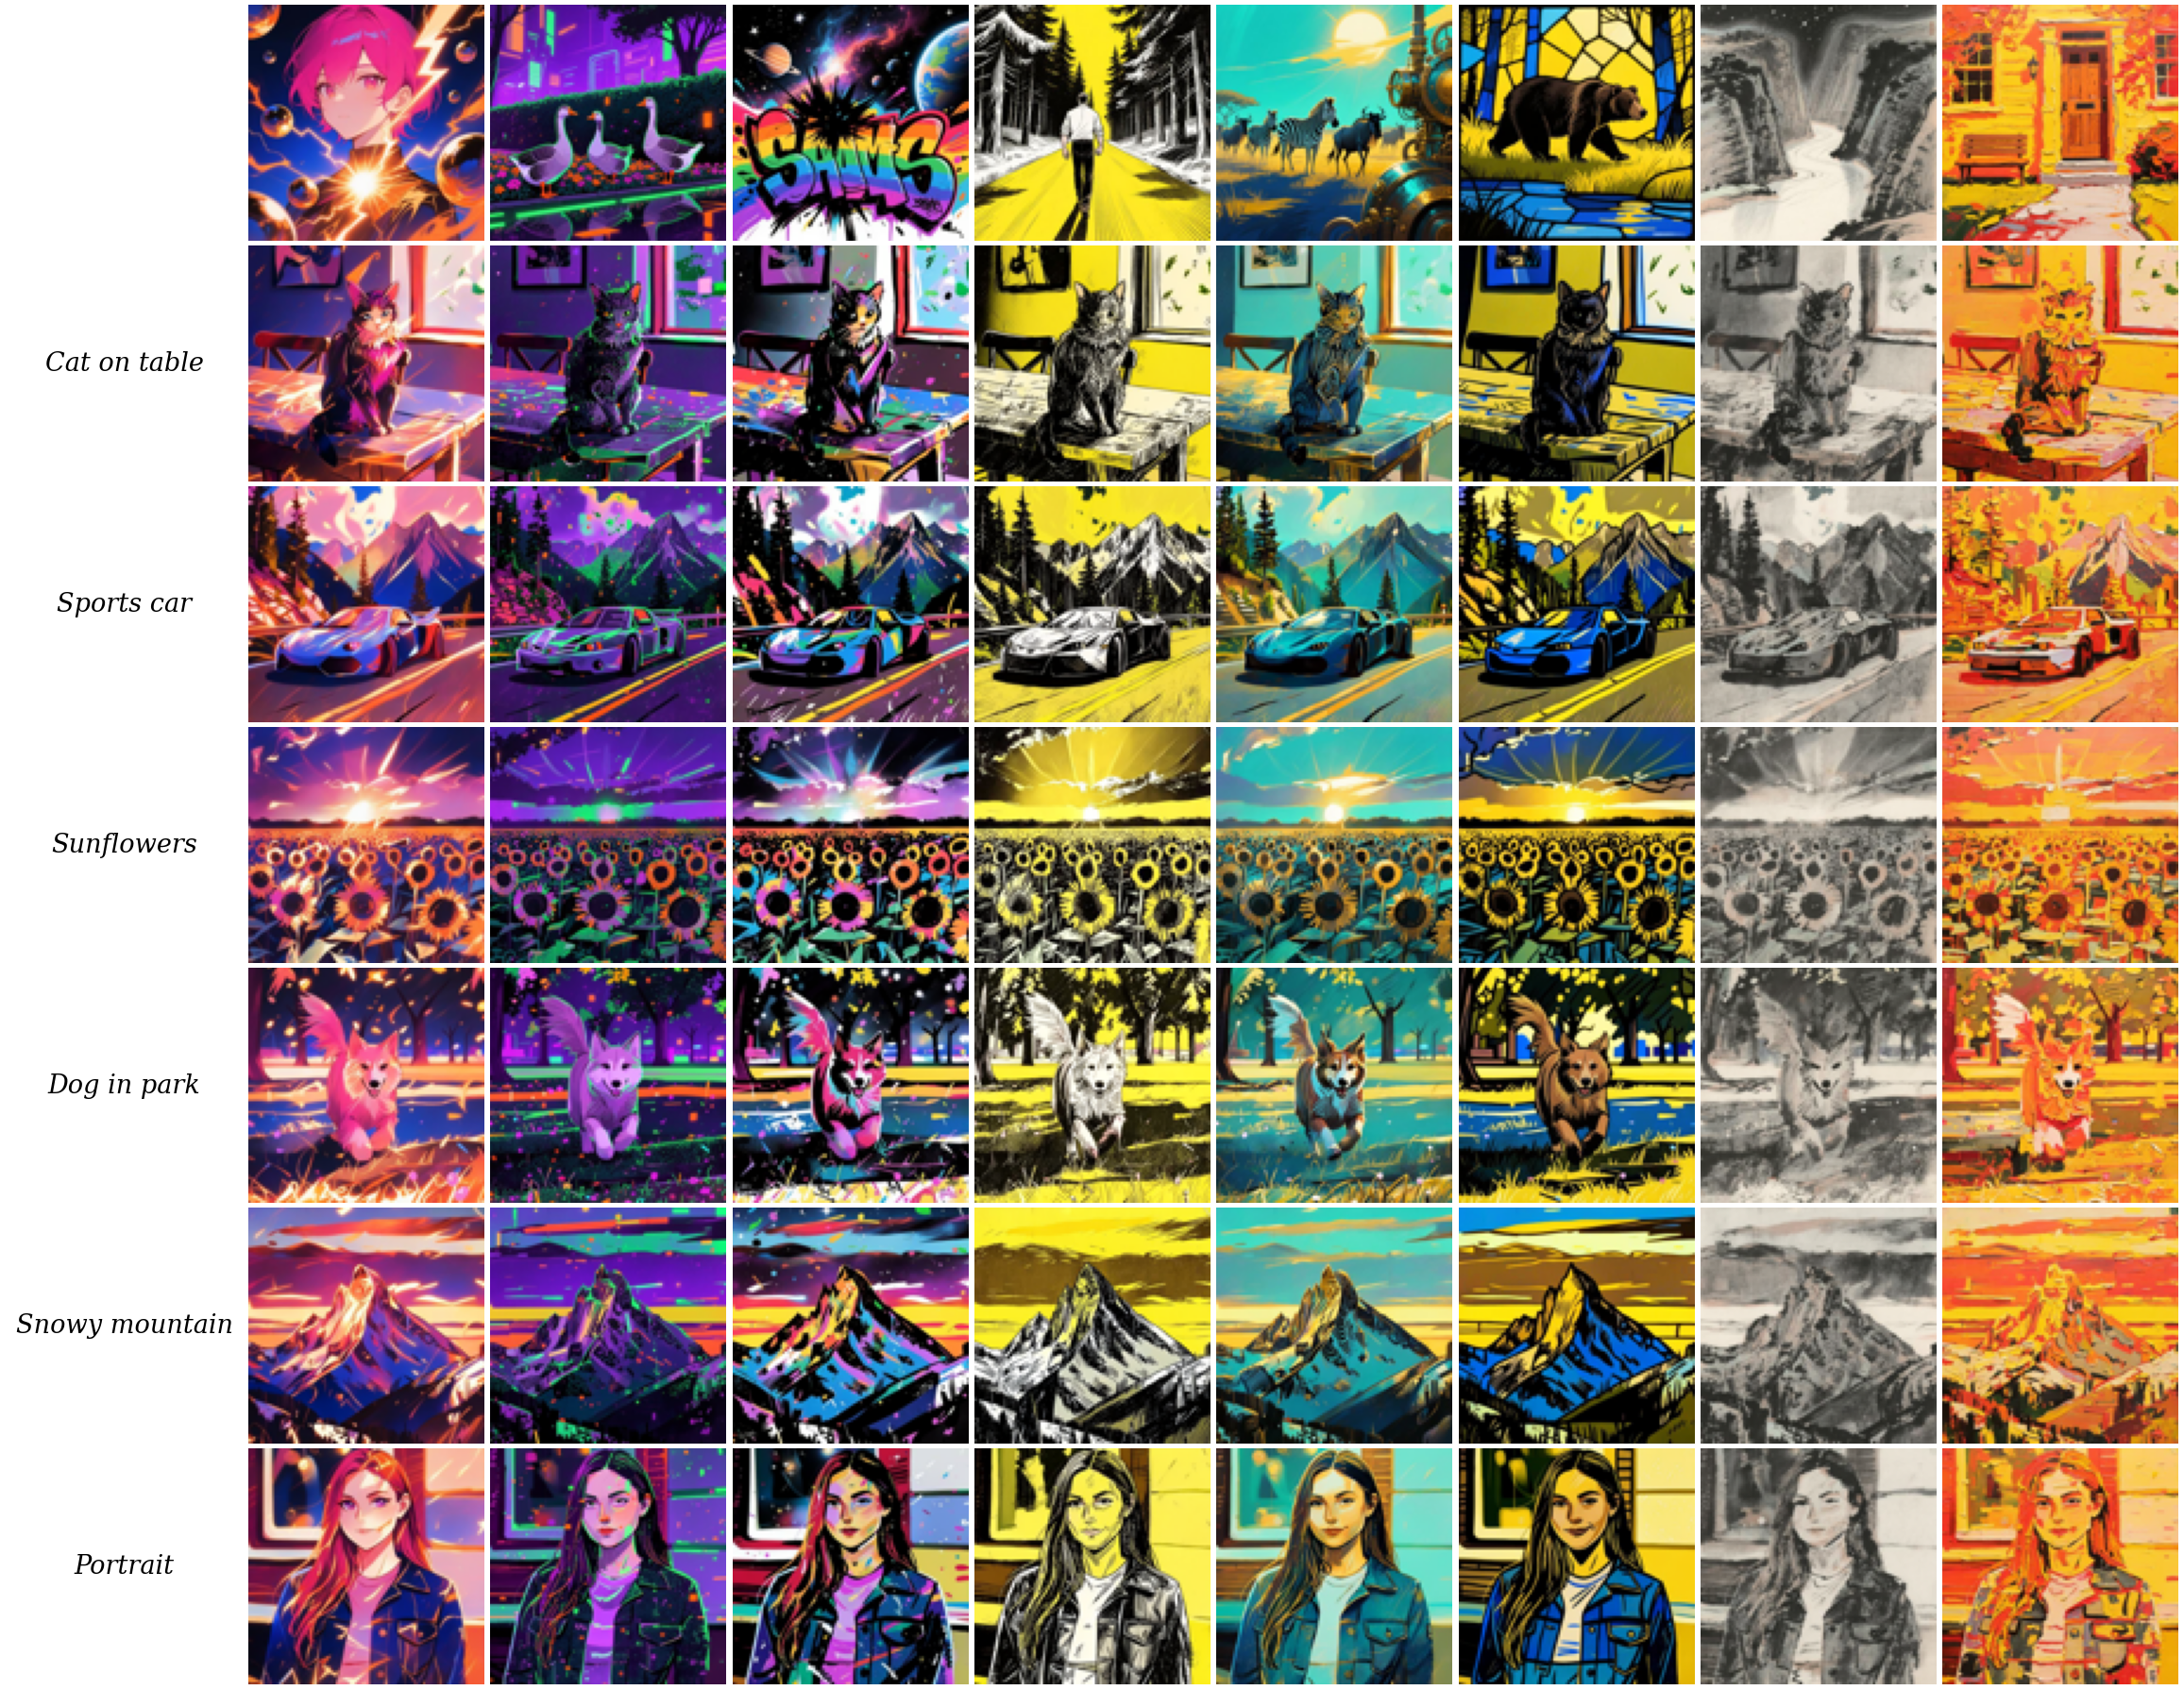
\includegraphics[width=\linewidth]{figures_hires/fig12_t2i_benchmark.png}
  \caption{%
    T2I benchmark gallery: Hyperion (Ours) results for 6 content prompts
    $\times$ 8 diverse style references from the full 39-style benchmark.
    \emph{Columns} (left to right): anime cel, cyberpunk neon, graffiti, comic
    book, steampunk, stained glass, Chinese ink wash, oil impasto.
    \emph{Rows} (top to bottom): style reference, then the six content prompts
    p0--p5 of Table~\ref{tab:prompts} (cat on a wooden table, sports car on a
    mountain road, field of sunflowers, dog in a park, snowy mountain peak,
    portrait of a young woman).
    The method transfers sharply distinct media---vivid cel shading, neon glow,
    spray-paint lettering, halftone comic ink, ornate metalwork, leaded glass,
    monochrome ink, and thick impasto---while preserving prompt-specified subject
    identity and composition across the full style gamut.%
  }
  \label{fig:t2i_benchmark}
\end{figure}

Fig.~\ref{fig:vshuffle_cmp} contrasts our Hyperion with our faithful MM-DiT
adaptation of V-Shuffle, the representative training-free
\emph{value-manipulation} baseline (Sec.~\ref{sec:exp:main}). Because V-Shuffle
spatially permutes the style value tokens, it sprays style statistics across the
canvas without the cross-token gradient coupling that assembles coherent
brushstroke structure: on the Klein-9B MM-DiT this collapses into incoherent
texture mush in which the prompted subject is barely legible, so its style
fidelity is far below ours in every row.

The pairing makes the paper's central measurement point concrete. Over the full
$234$-pair benchmark our Hyperion \emph{dominates} V-Shuffle on both axes---CSD
$0.640$ vs.\ $0.232$ ($t{=}{+}47.9$, winning all $234/234$ pairs) and CLIP-T
$0.296$ vs.\ $0.230$ ($t{=}{+}16.5$). Value permutation severs the
style--content correspondence: it neither transfers coherent style nor preserves
the prompt, directly illustrating that coherent style requires the cross-token
coupling of a backward pass (Sec.~\ref{sec:discussion:metrics}).

% 十修排版: fig:vshuffle_cmp 与 fig:i2i_ext 合并为同一浮动页（同上，编号不变），
% 原 vshuffle 图独占页仅用右上角四分之一，是全文最大的空白页。
\begin{figure}[!tp]
  \centering
  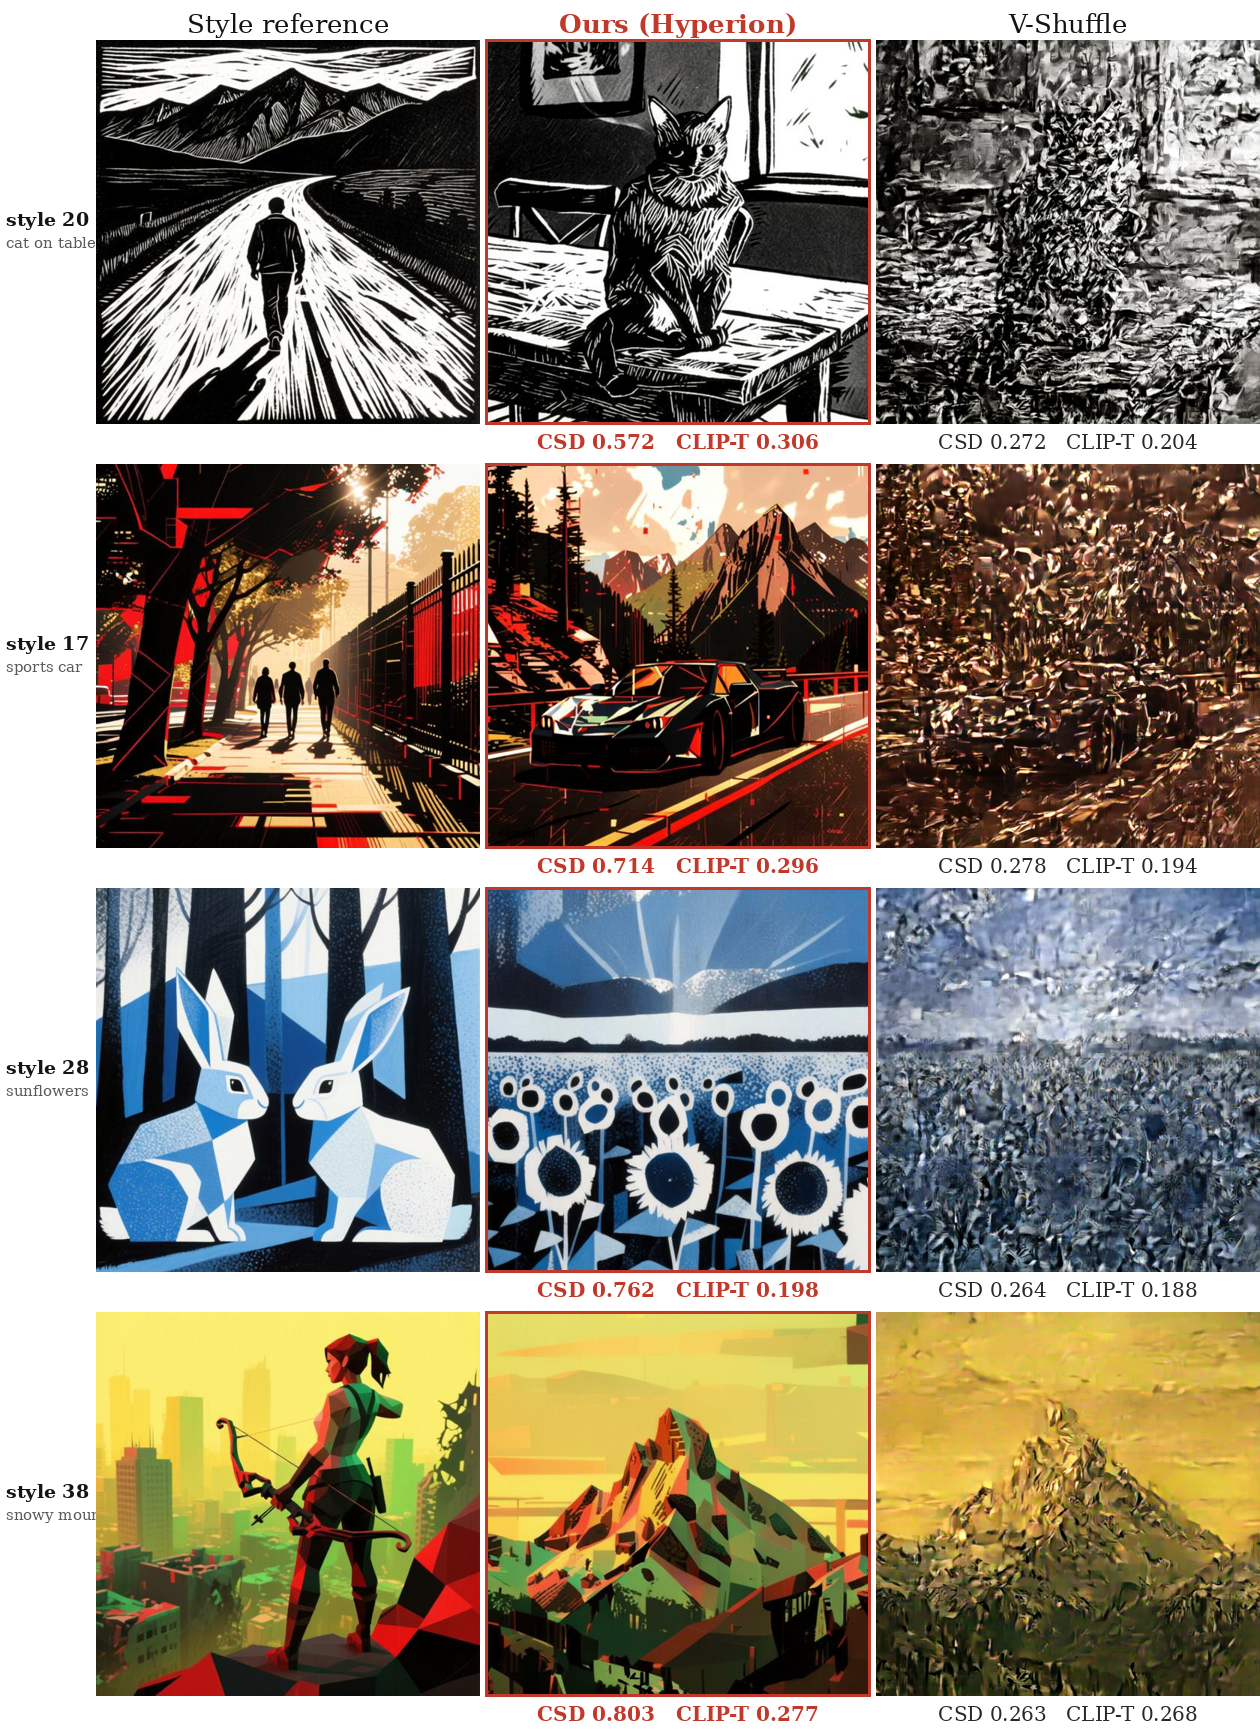
\includegraphics[width=0.62\linewidth]{figures_hires/fig19_vshuffle_cmp.png}
  \caption{%
    Qualitative comparison with our faithful MM-DiT adaptation of
    V-Shuffle~\cite{vshuffle2025}, the representative training-free
    value-manipulation method.
    \emph{Columns}: style reference, \textbf{Ours} (Hyperion), V-Shuffle (faithful
    full-injection adaptation); per-image CSD and CLIP-T annotated.
    The rows are representative pairs (V-Shuffle CSD near its dataset median, not
    worst cases). On Klein-9B, value permutation transfers only a weak, washed-out
    palette with degraded subject structure, whereas our Hyperion produces faithful
    style with an intact subject (full-benchmark statistics above).%
  }
  \label{fig:vshuffle_cmp}

  \vspace{2.5ex}
  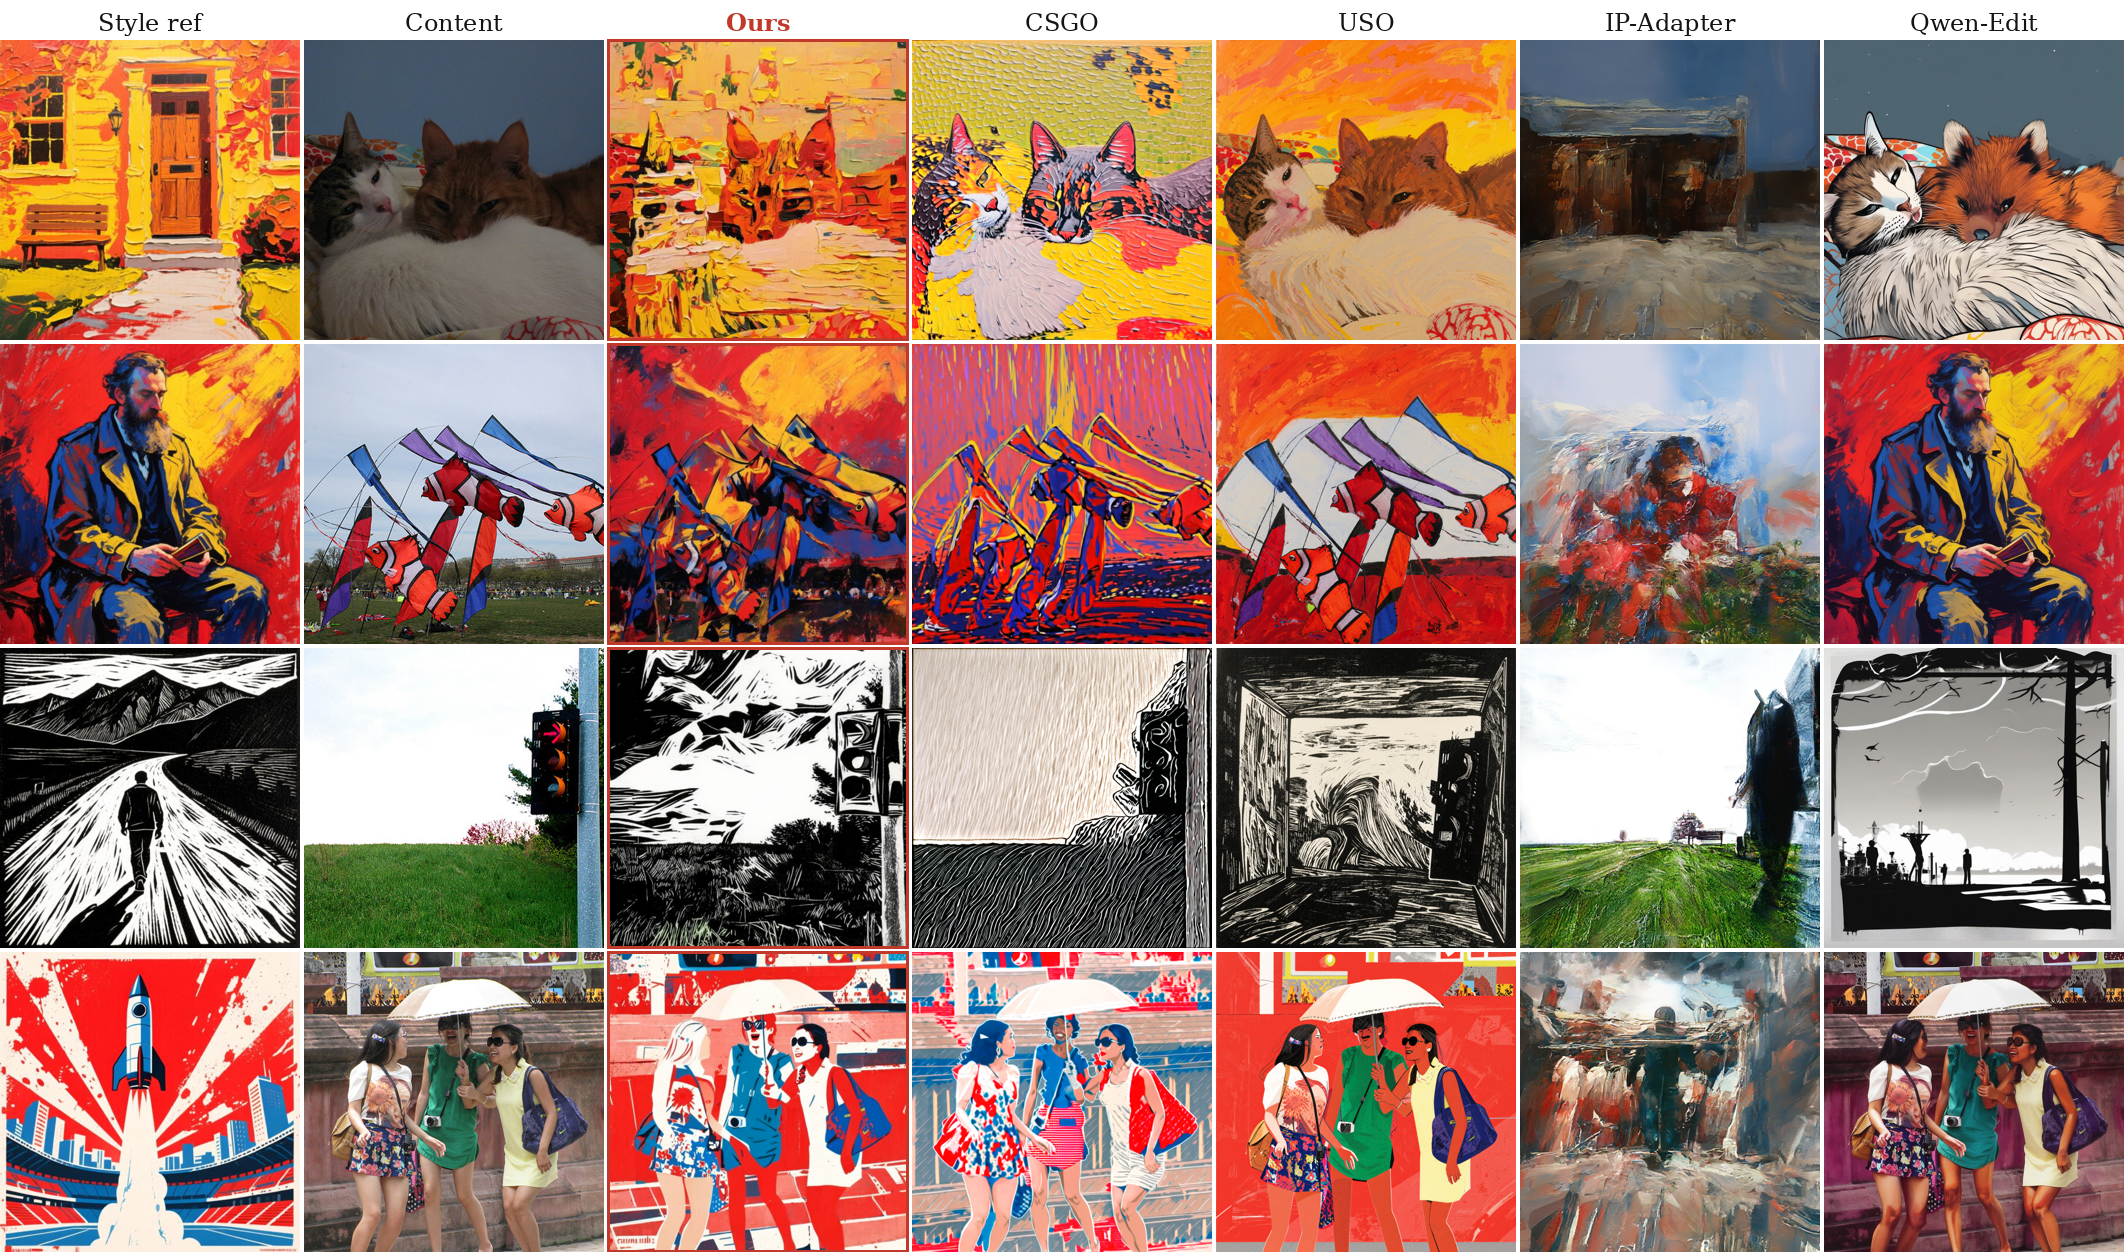
\includegraphics[width=\linewidth]{figures_hires/fig21_i2i_ext.png}
  \caption{%
    I2I comparison with trained style-transfer methods (Table~\ref{tab:i2i_ext}).
    \emph{Columns}: style reference, content image, \textbf{Ours} (Hyperion), CSGO,
    USO, IP-Adapter, Qwen-Image-Edit. Our training-free Hyperion transfers the
    strongest, most coherent style while preserving content; IP-Adapter applies
    only a generic painterly cast that weakly matches the specific reference
    (CSD~$0.160$); CSGO/USO/Qwen-Edit transfer partial or weaker style. Rows:
    content--style pairs (cnt00/sty27, cnt04/sty10, cnt08/sty20, cnt17/sty33).%
  }
  \label{fig:i2i_ext}
\end{figure}

\begin{table}[t]
  \centering
  \caption{I2I style transfer ablation (40-pair subset: 8 styles $\times$
           5 content images). STM is the Style--Texture Match
           (Sec.~\ref{sec:exp:texcoh}).}
  \label{tab:i2i}
  \footnotesize
  \begin{tabular}{lccccc}
    \toprule
    Method & CSD~$\uparrow$ & CLIP-T~$\uparrow$ & CLIP-I~$\uparrow$ & STM~$\uparrow$ & Fwd. \\
    \midrule
    Text-only (I2I) & 0.106 & 0.205 & 0.868 & 0.466 & 1 \\
    AdaIN (I2I)     & 0.155 & 0.208 & 0.863 & 0.486 & 2 \\
    Adam-8 (I2I)    & 0.649 & 0.224 & 0.695 & 0.673 & 10 \\
    \textbf{Hyperion (I2I)}    & \textbf{0.696} & 0.223 & 0.670 & \textbf{0.716} & 4 \\
    \bottomrule
  \end{tabular}
\end{table}

% 十修排版: fig:i2i_qual 与 fig:native_cmp 合并为同一浮动页（同上，编号不变）。
\begin{figure}[!tp]
  \centering
  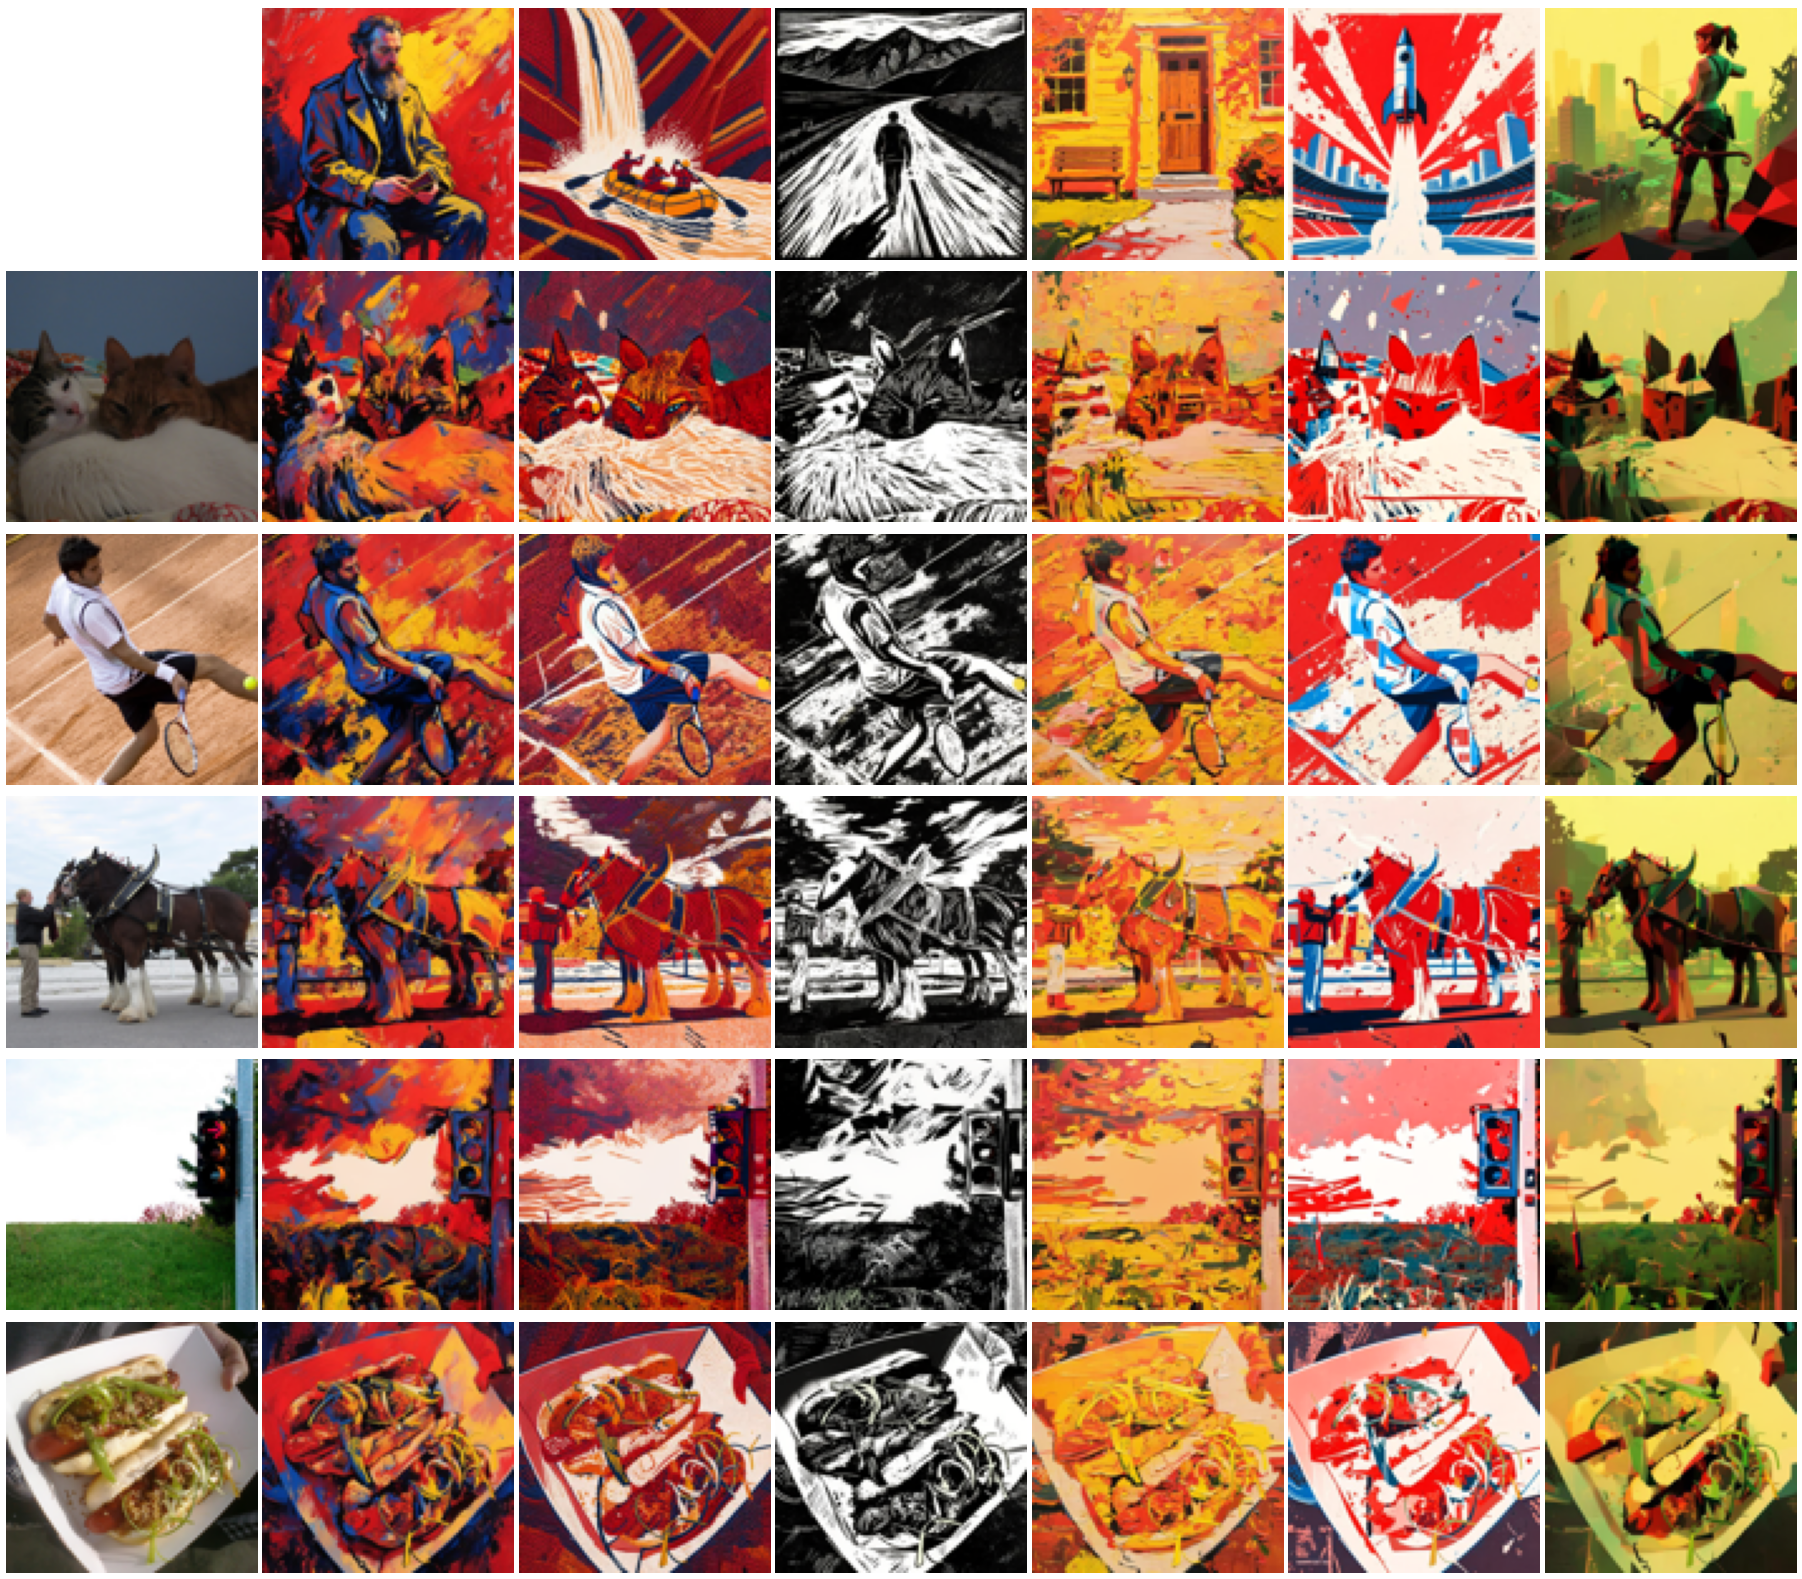
\includegraphics[width=0.92\linewidth]{figures_hires/fig10_qualitative_i2i.png}
  \caption{%
    Qualitative I2I results across 5 content images (rows) $\times$ 6 style
    references (top row); the top-left cell is intentionally blank.
    Content structure (object identity, spatial layout, fine-grained details)
    is preserved while style characteristics---brushstroke direction, color
    palette, textural grain---are faithfully transferred.
    Hyperion (Ours) delivers texture quality comparable to Adam-8 at $2.5\times$
    lower forward-pass cost.%
  }
  \label{fig:i2i_qual}

  \vspace{2.5ex}
  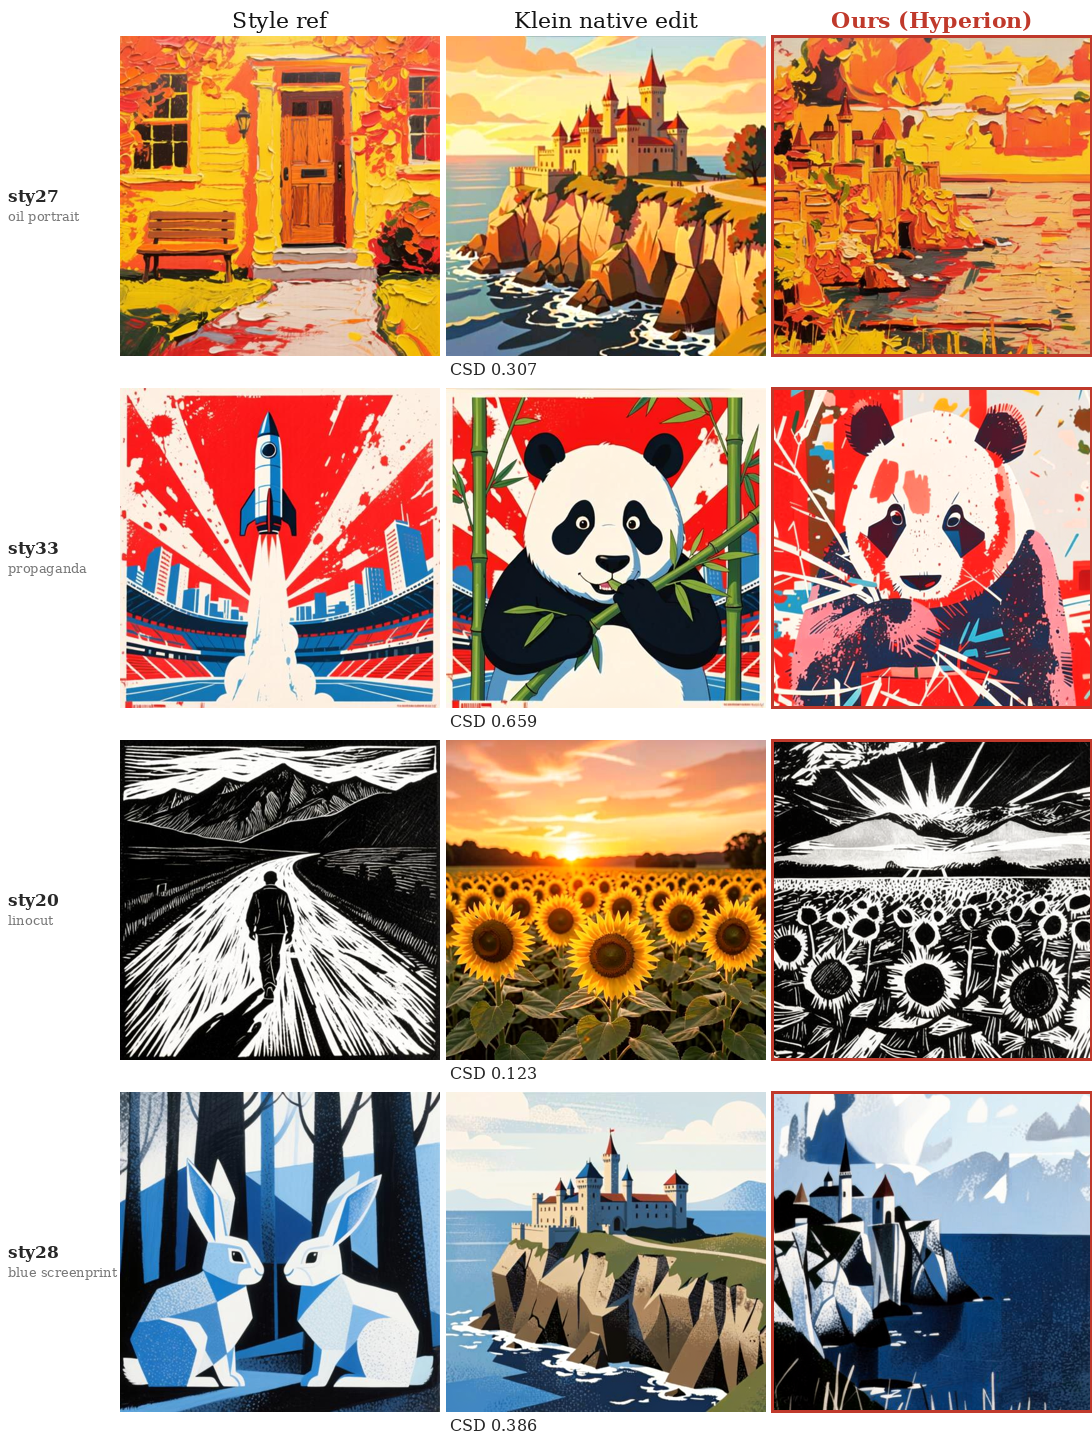
\includegraphics[width=0.86\linewidth]{figures_hires/fig_native_cmp.png}
  \caption{Klein-9B \emph{native} in-context edit vs.\ \textbf{Ours}. Prompting
    the frozen backbone to restyle the content directly (style image as the
    native \texttt{edit\_image}; no SLT, no Adam, no style forward) transfers
    style inconsistently---it often reverts to a literal, weakly-stylized
    rendering (per-image CSD annotated)---whereas our explicit pipeline applies
    the reference style faithfully. Over the 40-pair subset native edit reaches
    only CSD~$0.487$ and fails (CSD~$<0.30$) on $25\%$ of pairs vs.\ $0\%$ for
    Hyperion.}
  \label{fig:native_cmp}
\end{figure}


\end{document}
